\documentclass[twoside]{book}

% Packages required by doxygen
\usepackage{fixltx2e}
\usepackage{calc}
\usepackage{doxygen}
\usepackage[export]{adjustbox} % also loads graphicx
\usepackage{graphicx}
\usepackage[utf8]{inputenc}
\usepackage{makeidx}
\usepackage{multicol}
\usepackage{multirow}
\PassOptionsToPackage{warn}{textcomp}
\usepackage{textcomp}
\usepackage[nointegrals]{wasysym}
\usepackage[table]{xcolor}

% Font selection
\usepackage[T1]{fontenc}
\usepackage[scaled=.90]{helvet}
\usepackage{courier}
\usepackage{amssymb}
\usepackage{sectsty}
\renewcommand{\familydefault}{\sfdefault}
\allsectionsfont{%
  \fontseries{bc}\selectfont%
  \color{darkgray}%
}
\renewcommand{\DoxyLabelFont}{%
  \fontseries{bc}\selectfont%
  \color{darkgray}%
}
\newcommand{\+}{\discretionary{\mbox{\scriptsize$\hookleftarrow$}}{}{}}

% Page & text layout
\usepackage{geometry}
\geometry{%
  a4paper,%
  top=2.5cm,%
  bottom=2.5cm,%
  left=2.5cm,%
  right=2.5cm%
}
\tolerance=750
\hfuzz=15pt
\hbadness=750
\setlength{\emergencystretch}{15pt}
\setlength{\parindent}{0cm}
\setlength{\parskip}{3ex plus 2ex minus 2ex}
\makeatletter
\renewcommand{\paragraph}{%
  \@startsection{paragraph}{4}{0ex}{-1.0ex}{1.0ex}{%
    \normalfont\normalsize\bfseries\SS@parafont%
  }%
}
\renewcommand{\subparagraph}{%
  \@startsection{subparagraph}{5}{0ex}{-1.0ex}{1.0ex}{%
    \normalfont\normalsize\bfseries\SS@subparafont%
  }%
}
\makeatother

% Headers & footers
\usepackage{fancyhdr}
\pagestyle{fancyplain}
\fancyhead[LE]{\fancyplain{}{\bfseries\thepage}}
\fancyhead[CE]{\fancyplain{}{}}
\fancyhead[RE]{\fancyplain{}{\bfseries\leftmark}}
\fancyhead[LO]{\fancyplain{}{\bfseries\rightmark}}
\fancyhead[CO]{\fancyplain{}{}}
\fancyhead[RO]{\fancyplain{}{\bfseries\thepage}}
\fancyfoot[LE]{\fancyplain{}{}}
\fancyfoot[CE]{\fancyplain{}{}}
\fancyfoot[RE]{\fancyplain{}{\bfseries\scriptsize 構築\+: Doxygen }}
\fancyfoot[LO]{\fancyplain{}{\bfseries\scriptsize 構築\+: Doxygen }}
\fancyfoot[CO]{\fancyplain{}{}}
\fancyfoot[RO]{\fancyplain{}{}}
\renewcommand{\footrulewidth}{0.4pt}
\renewcommand{\chaptermark}[1]{%
  \markboth{#1}{}%
}
\renewcommand{\sectionmark}[1]{%
  \markright{\thesection\ #1}%
}

% Indices & bibliography
\usepackage{natbib}
\usepackage[titles]{tocloft}
\setcounter{tocdepth}{3}
\setcounter{secnumdepth}{5}
\makeindex

% Hyperlinks (required, but should be loaded last)
\usepackage{ifpdf}
\ifpdf
  \usepackage[pdftex,pagebackref=true]{hyperref}
\else
  \usepackage[ps2pdf,pagebackref=true]{hyperref}
\fi
\hypersetup{%
  colorlinks=true,%
  linkcolor=blue,%
  citecolor=blue,%
  unicode%
}

% Custom commands
\newcommand{\clearemptydoublepage}{%
  \newpage{\pagestyle{empty}\cleardoublepage}%
}

\usepackage{caption}
\captionsetup{labelsep=space,justification=centering,font={bf},singlelinecheck=off,skip=4pt,position=top}

%===== C O N T E N T S =====

\begin{document}

% Titlepage & ToC
\hypersetup{pageanchor=false,
             bookmarksnumbered=true,
             pdfencoding=unicode
            }
\pagenumbering{roman}
\begin{titlepage}
\vspace*{7cm}
\begin{center}%
{\Large D3\+D11\+A\+PI }\\
\vspace*{1cm}
{\large 構築\+: Doxygen 1.8.11}\\
\end{center}
\end{titlepage}
\clearemptydoublepage
\tableofcontents
\clearemptydoublepage
\pagenumbering{arabic}
\hypersetup{pageanchor=true}

%--- Begin generated contents ---
\chapter{名前空間索引}
\section{名前空間一覧}
詳解が付いた名前空間の一覧です。\begin{DoxyCompactList}
\item\contentsline{section}{\hyperlink{namespace_a_p_i}{A\+PI} \\*A\+P\+I名前空間に含める }{\pageref{namespace_a_p_i}}{}
\item\contentsline{section}{\hyperlink{namespace_d3_d11}{D3\+D11} }{\pageref{namespace_d3_d11}}{}
\item\contentsline{section}{\hyperlink{namespace_d3_d11_1_1_graphic}{D3\+D11\+::\+Graphic} }{\pageref{namespace_d3_d11_1_1_graphic}}{}
\item\contentsline{section}{\hyperlink{namespace_d3_d11_1_1_sound}{D3\+D11\+::\+Sound} }{\pageref{namespace_d3_d11_1_1_sound}}{}
\item\contentsline{section}{\hyperlink{namespace_key_code}{Key\+Code} \\*名前空間 }{\pageref{namespace_key_code}}{}
\end{DoxyCompactList}

\chapter{階層索引}
\section{クラス階層}
クラス階層一覧です。大雑把に文字符号順で並べられています。\begin{DoxyCompactList}
\item \contentsline{section}{abstract}{\pageref{class_a_p_i_1_1abstract}}{}
\item \contentsline{section}{Color}{\pageref{class_color}}{}
\item \contentsline{section}{C\+O\+N\+S\+T\+A\+N\+T\+\_\+\+B\+U\+F\+F\+E\+R\+\_\+\+B\+A\+SE}{\pageref{struct_d3_d11_1_1_graphic_1_1_c_o_n_s_t_a_n_t___b_u_f_f_e_r___b_a_s_e}}{}
\begin{DoxyCompactList}
\item \contentsline{section}{Sprite\+Shader\+Buffer}{\pageref{struct_d3_d11_1_1_graphic_1_1_sprite_shader_buffer}}{}
\end{DoxyCompactList}
\item \contentsline{section}{Debug}{\pageref{class_debug}}{}
\item \contentsline{section}{Game\+Pad}{\pageref{class_game_pad}}{}
\item I\+Texture\begin{DoxyCompactList}
\item \contentsline{section}{Texture}{\pageref{class_a_p_i_1_1_texture}}{}
\item \contentsline{section}{Texture\+Atlas}{\pageref{class_a_p_i_1_1_texture_atlas}}{}
\end{DoxyCompactList}
\item \contentsline{section}{Shader\+Data}{\pageref{struct_d3_d11_1_1_graphic_1_1_shader_data}}{}
\item \contentsline{section}{Singleton$<$ T $>$}{\pageref{class_singleton}}{}
\item \contentsline{section}{Singleton$<$ Audio\+Master $>$}{\pageref{class_singleton}}{}
\begin{DoxyCompactList}
\item \contentsline{section}{Audio\+Master}{\pageref{class_d3_d11_1_1_sound_1_1_audio_master}}{}
\end{DoxyCompactList}
\item \contentsline{section}{Singleton$<$ Camera $>$}{\pageref{class_singleton}}{}
\begin{DoxyCompactList}
\item \contentsline{section}{Camera}{\pageref{class_camera}}{}
\end{DoxyCompactList}
\item \contentsline{section}{Singleton$<$ Direct3\+D11 $>$}{\pageref{class_singleton}}{}
\begin{DoxyCompactList}
\item \contentsline{section}{Direct3\+D11}{\pageref{class_d3_d11_1_1_direct3_d11}}{}
\end{DoxyCompactList}
\item \contentsline{section}{Singleton$<$ Shader\+Manager $>$}{\pageref{class_singleton}}{}
\begin{DoxyCompactList}
\item \contentsline{section}{Shader\+Manager}{\pageref{class_d3_d11_1_1_graphic_1_1_shader_manager}}{}
\end{DoxyCompactList}
\item \contentsline{section}{Sprite}{\pageref{class_a_p_i_1_1_sprite}}{}
\item \contentsline{section}{V\+A\+R\+T\+E\+X\+\_\+\+B\+A\+SE}{\pageref{struct_d3_d11_1_1_graphic_1_1_v_a_r_t_e_x___b_a_s_e}}{}
\begin{DoxyCompactList}
\item \contentsline{section}{Sprite\+Vertex}{\pageref{struct_d3_d11_1_1_graphic_1_1_sprite_vertex}}{}
\end{DoxyCompactList}
\item \contentsline{section}{Wave}{\pageref{class_a_p_i_1_1_wave}}{}
\item \contentsline{section}{Window}{\pageref{class_window}}{}
\end{DoxyCompactList}

\chapter{クラス索引}
\section{クラス一覧}
クラス・構造体・共用体・インターフェースの一覧です。\begin{DoxyCompactList}
\item\contentsline{section}{\hyperlink{class_a_p_i_1_1abstract}{abstract} }{\pageref{class_a_p_i_1_1abstract}}{}
\item\contentsline{section}{\hyperlink{class_d3_d11_1_1_sound_1_1_audio_master}{Audio\+Master} }{\pageref{class_d3_d11_1_1_sound_1_1_audio_master}}{}
\item\contentsline{section}{\hyperlink{class_camera}{Camera} }{\pageref{class_camera}}{}
\item\contentsline{section}{\hyperlink{class_color}{Color} \\*カラークラス }{\pageref{class_color}}{}
\item\contentsline{section}{\hyperlink{struct_d3_d11_1_1_graphic_1_1_c_o_n_s_t_a_n_t___b_u_f_f_e_r___b_a_s_e}{C\+O\+N\+S\+T\+A\+N\+T\+\_\+\+B\+U\+F\+F\+E\+R\+\_\+\+B\+A\+SE} \\*シェーダー側に渡すコンスタントバッファの基底構造体 }{\pageref{struct_d3_d11_1_1_graphic_1_1_c_o_n_s_t_a_n_t___b_u_f_f_e_r___b_a_s_e}}{}
\item\contentsline{section}{\hyperlink{class_debug}{Debug} \\*デバッグ用シンボルの宣言  Releaseビルド時に有効にならないようマクロで囲む }{\pageref{class_debug}}{}
\item\contentsline{section}{\hyperlink{class_d3_d11_1_1_direct3_d11}{Direct3\+D11} \\*Direct3\+D11デバイスclass }{\pageref{class_d3_d11_1_1_direct3_d11}}{}
\item\contentsline{section}{\hyperlink{class_game_pad}{Game\+Pad} \\*ゲームパッドクラス  X\+B\+O\+Xコントローラーの入力制御クラス }{\pageref{class_game_pad}}{}
\item\contentsline{section}{\hyperlink{struct_d3_d11_1_1_graphic_1_1_shader_data}{Shader\+Data} \\*シェーダーを構成する構造体 }{\pageref{struct_d3_d11_1_1_graphic_1_1_shader_data}}{}
\item\contentsline{section}{\hyperlink{class_d3_d11_1_1_graphic_1_1_shader_manager}{Shader\+Manager} \\*シェーダー管理クラス  シェーダーを作成せずとも描画出来るデフォルトシェーダーを用意する }{\pageref{class_d3_d11_1_1_graphic_1_1_shader_manager}}{}
\item\contentsline{section}{\hyperlink{class_singleton}{Singleton$<$ T $>$} }{\pageref{class_singleton}}{}
\item\contentsline{section}{\hyperlink{class_a_p_i_1_1_sprite}{Sprite} }{\pageref{class_a_p_i_1_1_sprite}}{}
\item\contentsline{section}{\hyperlink{struct_d3_d11_1_1_graphic_1_1_sprite_shader_buffer}{Sprite\+Shader\+Buffer} \\*スプライトのコンスタントバッファ構造体 }{\pageref{struct_d3_d11_1_1_graphic_1_1_sprite_shader_buffer}}{}
\item\contentsline{section}{\hyperlink{struct_d3_d11_1_1_graphic_1_1_sprite_vertex}{Sprite\+Vertex} \\*スプライトの頂点構造体 }{\pageref{struct_d3_d11_1_1_graphic_1_1_sprite_vertex}}{}
\item\contentsline{section}{\hyperlink{class_a_p_i_1_1_texture}{Texture} }{\pageref{class_a_p_i_1_1_texture}}{}
\item\contentsline{section}{\hyperlink{class_a_p_i_1_1_texture_atlas}{Texture\+Atlas} }{\pageref{class_a_p_i_1_1_texture_atlas}}{}
\item\contentsline{section}{\hyperlink{struct_d3_d11_1_1_graphic_1_1_v_a_r_t_e_x___b_a_s_e}{V\+A\+R\+T\+E\+X\+\_\+\+B\+A\+SE} \\*基底頂点構造体 }{\pageref{struct_d3_d11_1_1_graphic_1_1_v_a_r_t_e_x___b_a_s_e}}{}
\item\contentsline{section}{\hyperlink{class_a_p_i_1_1_wave}{Wave} }{\pageref{class_a_p_i_1_1_wave}}{}
\item\contentsline{section}{\hyperlink{class_window}{Window} }{\pageref{class_window}}{}
\end{DoxyCompactList}

\chapter{ファイル索引}
\section{ファイル一覧}
詳解が付けられているファイルの一覧です。\begin{DoxyCompactList}
\item\contentsline{section}{C\+:/\+Users/yuuki/\+Desktop/\+Doxygen\+\_\+lib\+\_\+source/include/{\bfseries Audio\+Master.\+h} }{\pageref{_audio_master_8h}}{}
\item\contentsline{section}{C\+:/\+Users/yuuki/\+Desktop/\+Doxygen\+\_\+lib\+\_\+source/include/{\bfseries Camera.\+h} }{\pageref{_camera_8h}}{}
\item\contentsline{section}{C\+:/\+Users/yuuki/\+Desktop/\+Doxygen\+\_\+lib\+\_\+source/include/{\bfseries Color.\+h} }{\pageref{_color_8h}}{}
\item\contentsline{section}{C\+:/\+Users/yuuki/\+Desktop/\+Doxygen\+\_\+lib\+\_\+source/include/\hyperlink{_debug_8cpp}{Debug.\+cpp} \\*デバッグ関連のクラス  各クラスで使われているシンボルの宣言も含める 参照は不要なのでメンバは全てstaticで宣言及び定義 }{\pageref{_debug_8cpp}}{}
\item\contentsline{section}{C\+:/\+Users/yuuki/\+Desktop/\+Doxygen\+\_\+lib\+\_\+source/include/\hyperlink{_debug_8h}{Debug.\+h} \\*デバッグ関連のクラス  各クラスで使われているシンボルの宣言も含める 参照は不要なのでメンバは全てstaticで宣言及び定義 }{\pageref{_debug_8h}}{}
\item\contentsline{section}{C\+:/\+Users/yuuki/\+Desktop/\+Doxygen\+\_\+lib\+\_\+source/include/{\bfseries Direct3\+D11.\+h} }{\pageref{_direct3_d11_8h}}{}
\item\contentsline{section}{C\+:/\+Users/yuuki/\+Desktop/\+Doxygen\+\_\+lib\+\_\+source/include/{\bfseries Game\+Pad.\+h} }{\pageref{_game_pad_8h}}{}
\item\contentsline{section}{C\+:/\+Users/yuuki/\+Desktop/\+Doxygen\+\_\+lib\+\_\+source/include/{\bfseries I\+Texture.\+h} }{\pageref{_i_texture_8h}}{}
\item\contentsline{section}{C\+:/\+Users/yuuki/\+Desktop/\+Doxygen\+\_\+lib\+\_\+source/include/{\bfseries Memory\+Leaks.\+h} }{\pageref{_memory_leaks_8h}}{}
\item\contentsline{section}{C\+:/\+Users/yuuki/\+Desktop/\+Doxygen\+\_\+lib\+\_\+source/include/{\bfseries My\+Game.\+h} }{\pageref{_my_game_8h}}{}
\item\contentsline{section}{C\+:/\+Users/yuuki/\+Desktop/\+Doxygen\+\_\+lib\+\_\+source/include/{\bfseries Shader\+Manager.\+h} }{\pageref{_shader_manager_8h}}{}
\item\contentsline{section}{C\+:/\+Users/yuuki/\+Desktop/\+Doxygen\+\_\+lib\+\_\+source/include/{\bfseries Singleton.\+h} }{\pageref{_singleton_8h}}{}
\item\contentsline{section}{C\+:/\+Users/yuuki/\+Desktop/\+Doxygen\+\_\+lib\+\_\+source/include/{\bfseries Sprite.\+h} }{\pageref{_sprite_8h}}{}
\item\contentsline{section}{C\+:/\+Users/yuuki/\+Desktop/\+Doxygen\+\_\+lib\+\_\+source/include/{\bfseries stdafx.\+h} }{\pageref{stdafx_8h}}{}
\item\contentsline{section}{C\+:/\+Users/yuuki/\+Desktop/\+Doxygen\+\_\+lib\+\_\+source/include/{\bfseries Struct\+Shader\+Base.\+h} }{\pageref{_struct_shader_base_8h}}{}
\item\contentsline{section}{C\+:/\+Users/yuuki/\+Desktop/\+Doxygen\+\_\+lib\+\_\+source/include/{\bfseries targetver.\+h} }{\pageref{targetver_8h}}{}
\item\contentsline{section}{C\+:/\+Users/yuuki/\+Desktop/\+Doxygen\+\_\+lib\+\_\+source/include/{\bfseries Texture.\+h} }{\pageref{_texture_8h}}{}
\item\contentsline{section}{C\+:/\+Users/yuuki/\+Desktop/\+Doxygen\+\_\+lib\+\_\+source/include/{\bfseries Texture\+Atlas.\+h} }{\pageref{_texture_atlas_8h}}{}
\item\contentsline{section}{C\+:/\+Users/yuuki/\+Desktop/\+Doxygen\+\_\+lib\+\_\+source/include/{\bfseries Wave.\+h} }{\pageref{_wave_8h}}{}
\item\contentsline{section}{C\+:/\+Users/yuuki/\+Desktop/\+Doxygen\+\_\+lib\+\_\+source/include/{\bfseries W\+I\+C\+Texture\+Loader.\+h} }{\pageref{_w_i_c_texture_loader_8h}}{}
\item\contentsline{section}{C\+:/\+Users/yuuki/\+Desktop/\+Doxygen\+\_\+lib\+\_\+source/include/\hyperlink{_window_8cpp}{Window.\+cpp} \\*Windows\+A\+P\+Iのウィンドウ生成 }{\pageref{_window_8cpp}}{}
\item\contentsline{section}{C\+:/\+Users/yuuki/\+Desktop/\+Doxygen\+\_\+lib\+\_\+source/include/\hyperlink{_window_8h}{Window.\+h} \\*Windows\+A\+P\+Iのウィンドウ生成 }{\pageref{_window_8h}}{}
\end{DoxyCompactList}

\chapter{名前空間詳解}
\hypertarget{namespace_a_p_i}{}\section{A\+PI 名前空間}
\label{namespace_a_p_i}\index{A\+PI@{A\+PI}}


A\+P\+I名前空間に含める  


\subsection*{クラス}
\begin{DoxyCompactItemize}
\item 
class \hyperlink{class_a_p_i_1_1abstract}{abstract}
\item 
class \hyperlink{class_a_p_i_1_1_sprite}{Sprite}
\item 
class \hyperlink{class_a_p_i_1_1_texture}{Texture}
\item 
class \hyperlink{class_a_p_i_1_1_texture_atlas}{Texture\+Atlas}
\item 
class \hyperlink{class_a_p_i_1_1_wave}{Wave}
\end{DoxyCompactItemize}


\subsection{詳解}
A\+P\+I名前空間に含める 

A\+P\+I関連の名前空間に含める

A\+P\+Iの名前空間に含める

A\+P\+I名前空間に含める 
\hypertarget{namespace_d3_d11}{}\section{D3\+D11 名前空間}
\label{namespace_d3_d11}\index{D3\+D11@{D3\+D11}}
\subsection*{名前空間}
\begin{DoxyCompactItemize}
\item 
 \hyperlink{namespace_d3_d11_1_1_graphic}{Graphic}
\item 
 \hyperlink{namespace_d3_d11_1_1_sound}{Sound}
\end{DoxyCompactItemize}
\subsection*{クラス}
\begin{DoxyCompactItemize}
\item 
class \hyperlink{class_d3_d11_1_1_direct3_d11}{Direct3\+D11}
\begin{DoxyCompactList}\small\item\em Direct3\+D11デバイスclass. \end{DoxyCompactList}\end{DoxyCompactItemize}


\subsection{詳解}
Direct3\+D11関連

Direct3\+D11関連の名前空間 
\hypertarget{namespace_d3_d11_1_1_graphic}{}\section{D3\+D11\+:\+:Graphic 名前空間}
\label{namespace_d3_d11_1_1_graphic}\index{D3\+D11\+::\+Graphic@{D3\+D11\+::\+Graphic}}
\subsection*{クラス}
\begin{DoxyCompactItemize}
\item 
struct \hyperlink{struct_d3_d11_1_1_graphic_1_1_c_o_n_s_t_a_n_t___b_u_f_f_e_r___b_a_s_e}{C\+O\+N\+S\+T\+A\+N\+T\+\_\+\+B\+U\+F\+F\+E\+R\+\_\+\+B\+A\+SE}
\begin{DoxyCompactList}\small\item\em シェーダー側に渡すコンスタントバッファの基底構造体 \end{DoxyCompactList}\item 
struct \hyperlink{struct_d3_d11_1_1_graphic_1_1_shader_data}{Shader\+Data}
\begin{DoxyCompactList}\small\item\em シェーダーを構成する構造体 \end{DoxyCompactList}\item 
class \hyperlink{class_d3_d11_1_1_graphic_1_1_shader_manager}{Shader\+Manager}
\begin{DoxyCompactList}\small\item\em シェーダー管理クラス  シェーダーを作成せずとも描画出来るデフォルトシェーダーを用意する \end{DoxyCompactList}\item 
struct \hyperlink{struct_d3_d11_1_1_graphic_1_1_sprite_shader_buffer}{Sprite\+Shader\+Buffer}
\begin{DoxyCompactList}\small\item\em スプライトのコンスタントバッファ構造体 \end{DoxyCompactList}\item 
struct \hyperlink{struct_d3_d11_1_1_graphic_1_1_sprite_vertex}{Sprite\+Vertex}
\begin{DoxyCompactList}\small\item\em スプライトの頂点構造体 \end{DoxyCompactList}\item 
struct \hyperlink{struct_d3_d11_1_1_graphic_1_1_v_a_r_t_e_x___b_a_s_e}{V\+A\+R\+T\+E\+X\+\_\+\+B\+A\+SE}
\begin{DoxyCompactList}\small\item\em 基底頂点構造体 \end{DoxyCompactList}\end{DoxyCompactItemize}


\subsection{詳解}
描画関連の名前空間に含める

描画関連の名前空間 
\hypertarget{namespace_d3_d11_1_1_sound}{}\section{D3\+D11\+:\+:Sound 名前空間}
\label{namespace_d3_d11_1_1_sound}\index{D3\+D11\+::\+Sound@{D3\+D11\+::\+Sound}}
\subsection*{クラス}
\begin{DoxyCompactItemize}
\item 
class \hyperlink{class_d3_d11_1_1_sound_1_1_audio_master}{Audio\+Master}
\end{DoxyCompactItemize}


\subsection{詳解}
サウンド関連の名前空間に含める 
\hypertarget{namespace_key_code}{}\section{Key\+Code 名前空間}
\label{namespace_key_code}\index{Key\+Code@{Key\+Code}}


名前空間  


\subsection*{列挙型}
\begin{DoxyCompactItemize}
\item 
enum \hyperlink{namespace_key_code_a03bfec859eac87be20f8952c1eb89de0}{Button} \{ \\*
{\bfseries A}, 
{\bfseries B}, 
{\bfseries X}, 
{\bfseries Y}, 
\\*
{\bfseries S\+T\+A\+RT}, 
{\bfseries B\+A\+CK}, 
{\bfseries LB}, 
{\bfseries RB}, 
\\*
{\bfseries L\+\_\+\+S\+T\+I\+CK}, 
{\bfseries R\+\_\+\+S\+T\+I\+CK}
 \}\begin{DoxyCompactList}\small\item\em ボタンのキーコード列挙体 \end{DoxyCompactList}
\item 
enum \hyperlink{namespace_key_code_a68dc8420d4850fe68378bc682c360e30}{Trigger} \{ {\bfseries LT}, 
{\bfseries RT}
 \}\hypertarget{namespace_key_code_a68dc8420d4850fe68378bc682c360e30}{}\label{namespace_key_code_a68dc8420d4850fe68378bc682c360e30}
\begin{DoxyCompactList}\small\item\em トリガーのキーコード列挙体 \end{DoxyCompactList}
\item 
enum \hyperlink{namespace_key_code_af3282177b831055ef900d2bf53e100db}{Joy\+Stick} \{ {\bfseries L\+E\+FT}, 
{\bfseries R\+I\+G\+HT}
 \}\hypertarget{namespace_key_code_af3282177b831055ef900d2bf53e100db}{}\label{namespace_key_code_af3282177b831055ef900d2bf53e100db}
\begin{DoxyCompactList}\small\item\em ジョイスティックの種類列挙体 \end{DoxyCompactList}
\item 
enum \hyperlink{namespace_key_code_a16ba82423f2a8ac640d047568347eee4}{Arrow} \{ {\bfseries V\+E\+R\+T\+I\+C\+AL}, 
{\bfseries H\+O\+R\+I\+Z\+O\+N\+T\+AL}
 \}\hypertarget{namespace_key_code_a16ba82423f2a8ac640d047568347eee4}{}\label{namespace_key_code_a16ba82423f2a8ac640d047568347eee4}
\begin{DoxyCompactList}\small\item\em 方向キーのキーコード列挙体 \end{DoxyCompactList}
\end{DoxyCompactItemize}


\subsection{詳解}
名前空間 

\subsection{列挙型詳解}
\index{Key\+Code@{Key\+Code}!Button@{Button}}
\index{Button@{Button}!Key\+Code@{Key\+Code}}
\subsubsection[{\texorpdfstring{Button}{Button}}]{\setlength{\rightskip}{0pt plus 5cm}enum {\bf Button}}\hypertarget{namespace_key_code_a03bfec859eac87be20f8952c1eb89de0}{}\label{namespace_key_code_a03bfec859eac87be20f8952c1eb89de0}


ボタンのキーコード列挙体 

列挙体キーコード 
\chapter{クラス詳解}
\hypertarget{class_a_p_i_1_1abstract}{}\section{abstract クラス}
\label{class_a_p_i_1_1abstract}\index{abstract@{abstract}}
\subsection*{公開型}
\begin{DoxyCompactItemize}
\item 
enum \hyperlink{class_a_p_i_1_1abstract_a0a6f8b1d41f00f3b6bd7566adbcf4f36}{Tile\+Mode} \{ \\*
\hyperlink{class_a_p_i_1_1abstract_a0a6f8b1d41f00f3b6bd7566adbcf4f36a65cd6695b7f90c094cad51f9d69a1cbe}{Clamp} = D3\+D11\+\_\+\+T\+E\+X\+T\+U\+R\+E\+\_\+\+A\+D\+D\+R\+E\+S\+S\+\_\+\+M\+O\+DE\+:\+:D3\+D11\+\_\+\+T\+E\+X\+T\+U\+R\+E\+\_\+\+A\+D\+D\+R\+E\+S\+S\+\_\+\+C\+L\+A\+MP, 
\hyperlink{class_a_p_i_1_1abstract_a0a6f8b1d41f00f3b6bd7566adbcf4f36aa69f0f49b99456743880469971b657e5}{Border} = D3\+D11\+\_\+\+T\+E\+X\+T\+U\+R\+E\+\_\+\+A\+D\+D\+R\+E\+S\+S\+\_\+\+M\+O\+DE\+:\+:D3\+D11\+\_\+\+T\+E\+X\+T\+U\+R\+E\+\_\+\+A\+D\+D\+R\+E\+S\+S\+\_\+\+B\+O\+R\+D\+ER, 
{\bfseries Mirror\+Once} = D3\+D11\+\_\+\+T\+E\+X\+T\+U\+R\+E\+\_\+\+A\+D\+D\+R\+E\+S\+S\+\_\+\+M\+O\+DE\+:\+:D3\+D11\+\_\+\+T\+E\+X\+T\+U\+R\+E\+\_\+\+A\+D\+D\+R\+E\+S\+S\+\_\+\+M\+I\+R\+R\+O\+R\+\_\+\+O\+N\+CE, 
\hyperlink{class_a_p_i_1_1abstract_a0a6f8b1d41f00f3b6bd7566adbcf4f36a7794c24dd1265ef91cd516a6a2fa40a5}{Wrap} = D3\+D11\+\_\+\+T\+E\+X\+T\+U\+R\+E\+\_\+\+A\+D\+D\+R\+E\+S\+S\+\_\+\+M\+O\+DE\+:\+:D3\+D11\+\_\+\+T\+E\+X\+T\+U\+R\+E\+\_\+\+A\+D\+D\+R\+E\+S\+S\+\_\+\+W\+R\+AP, 
\\*
\hyperlink{class_a_p_i_1_1abstract_a0a6f8b1d41f00f3b6bd7566adbcf4f36a938cfe42fc80a4916f2e6eda40959e9a}{Mirror} = D3\+D11\+\_\+\+T\+E\+X\+T\+U\+R\+E\+\_\+\+A\+D\+D\+R\+E\+S\+S\+\_\+\+M\+O\+DE\+:\+:D3\+D11\+\_\+\+T\+E\+X\+T\+U\+R\+E\+\_\+\+A\+D\+D\+R\+E\+S\+S\+\_\+\+M\+I\+R\+R\+OR
 \}\begin{DoxyCompactList}\small\item\em タイリングモードの設定 \end{DoxyCompactList}
\item 
enum \hyperlink{class_a_p_i_1_1abstract_a520ef65de715096fdca5c71afa9273a1}{Filtering\+Mode} \{ \hyperlink{class_a_p_i_1_1abstract_a520ef65de715096fdca5c71afa9273a1a5b577e188dc4657a3e573fb2dae1a924}{Point} = D3\+D11\+\_\+\+F\+I\+L\+T\+ER\+:\+:D3\+D11\+\_\+\+F\+I\+L\+T\+E\+R\+\_\+\+M\+I\+N\+\_\+\+M\+A\+G\+\_\+\+M\+I\+P\+\_\+\+P\+O\+I\+NT, 
\hyperlink{class_a_p_i_1_1abstract_a520ef65de715096fdca5c71afa9273a1a657ab5c6571e53d74c63110cc8448c8b}{Bilinear} = D3\+D11\+\_\+\+F\+I\+L\+T\+ER\+:\+:D3\+D11\+\_\+\+F\+I\+L\+T\+E\+R\+\_\+\+M\+I\+N\+\_\+\+M\+A\+G\+\_\+\+L\+I\+N\+E\+A\+R\+\_\+\+M\+I\+P\+\_\+\+P\+O\+I\+NT, 
\hyperlink{class_a_p_i_1_1abstract_a520ef65de715096fdca5c71afa9273a1ab9db546b92309fcc8cfd67b7b6bbe8d2}{Trilinear} = D3\+D11\+\_\+\+F\+I\+L\+T\+ER\+:\+:D3\+D11\+\_\+\+F\+I\+L\+T\+E\+R\+\_\+\+M\+I\+N\+\_\+\+M\+A\+G\+\_\+\+M\+I\+P\+\_\+\+L\+I\+N\+E\+AR, 
\hyperlink{class_a_p_i_1_1abstract_a520ef65de715096fdca5c71afa9273a1a22690afbc2ee3a3ba2a141ab906f273c}{Anisotropic} = D3\+D11\+\_\+\+F\+I\+L\+T\+ER\+:\+:D3\+D11\+\_\+\+F\+I\+L\+T\+E\+R\+\_\+\+A\+N\+I\+S\+O\+T\+R\+O\+P\+IC
 \}\begin{DoxyCompactList}\small\item\em フィルタリングモードの設定 \end{DoxyCompactList}
\end{DoxyCompactItemize}
\subsection*{公開メンバ関数}
\begin{DoxyCompactItemize}
\item 
\hyperlink{class_a_p_i_1_1abstract_a296b1719c68831928574193a56a32791}{I\+Texture} ()\hypertarget{class_a_p_i_1_1abstract_a296b1719c68831928574193a56a32791}{}\label{class_a_p_i_1_1abstract_a296b1719c68831928574193a56a32791}

\begin{DoxyCompactList}\small\item\em コンストラクタ \end{DoxyCompactList}\item 
virtual \hyperlink{class_a_p_i_1_1abstract_a79a99935966ece5dbbd8be4439da47dd}{$\sim$\+I\+Texture} ()\hypertarget{class_a_p_i_1_1abstract_a79a99935966ece5dbbd8be4439da47dd}{}\label{class_a_p_i_1_1abstract_a79a99935966ece5dbbd8be4439da47dd}

\begin{DoxyCompactList}\small\item\em 仮想デストラクタ \end{DoxyCompactList}\item 
virtual void {\bfseries Finalize} ()\hypertarget{class_a_p_i_1_1abstract_a5659cae021514f6919def4b7f67402cf}{}\label{class_a_p_i_1_1abstract_a5659cae021514f6919def4b7f67402cf}

\item 
bool {\bfseries Set\+Size} (const Direct\+X\+::\+X\+M\+I\+N\+T2 size)\hypertarget{class_a_p_i_1_1abstract_ac3e510a817d37307e790d4d414e956b5}{}\label{class_a_p_i_1_1abstract_ac3e510a817d37307e790d4d414e956b5}

\item 
Direct\+X\+::\+X\+M\+I\+N\+T2 {\bfseries Get\+Size} () const \hypertarget{class_a_p_i_1_1abstract_a2e070ca1e8dfcf0404a2922dc1cd0bd6}{}\label{class_a_p_i_1_1abstract_a2e070ca1e8dfcf0404a2922dc1cd0bd6}

\item 
I\+D3\+D11\+Sampler\+State $\ast$$\ast$ {\bfseries Get\+Sampler\+State} ()\hypertarget{class_a_p_i_1_1abstract_adb362e0200295c54533c2491817ee356}{}\label{class_a_p_i_1_1abstract_adb362e0200295c54533c2491817ee356}

\item 
I\+D3\+D11\+Shader\+Resource\+View $\ast$$\ast$ {\bfseries Get\+Shader\+Resource\+View} ()\hypertarget{class_a_p_i_1_1abstract_ad03203b23b31f1b5c3dad3bdf9f979c3}{}\label{class_a_p_i_1_1abstract_ad03203b23b31f1b5c3dad3bdf9f979c3}

\item 
H\+R\+E\+S\+U\+LT \hyperlink{class_a_p_i_1_1abstract_aa58242e8408771bda104c984a0e476bd}{Set\+Tile\+And\+Filtering} (const \hyperlink{class_a_p_i_1_1abstract_a0a6f8b1d41f00f3b6bd7566adbcf4f36}{Tile\+Mode} tile\+Mode, const \hyperlink{class_a_p_i_1_1abstract_a520ef65de715096fdca5c71afa9273a1}{Filtering\+Mode} filter\+Mode)
\begin{DoxyCompactList}\small\item\em タイリングモードとフィルタリングモードの設定 \end{DoxyCompactList}\end{DoxyCompactItemize}
\subsection*{公開変数類}
\begin{DoxyCompactItemize}
\item 
\hyperlink{class_color}{Color} \hyperlink{class_a_p_i_1_1abstract_a91f4e4cb69b7fa77ce4c2f224d7980cc}{m\+\_\+\+Color}
\end{DoxyCompactItemize}
\subsection*{限定公開メンバ関数}
\begin{DoxyCompactItemize}
\item 
H\+R\+E\+S\+U\+LT \hyperlink{class_a_p_i_1_1abstract_ad78bf31f9df322ccdc67c509a0283a37}{Load} (std\+::string file\+Path)
\begin{DoxyCompactList}\small\item\em 画像の読み込みを行い\+S\+R\+Vを作成  W\+I\+Cを使い画像データを読み込み、\+S\+R\+Vを作成、メンバ変数にバインド \end{DoxyCompactList}\end{DoxyCompactItemize}
\subsection*{限定公開変数類}
\begin{DoxyCompactItemize}
\item 
\hyperlink{class_a_p_i_1_1abstract_a0a6f8b1d41f00f3b6bd7566adbcf4f36}{Tile\+Mode} \hyperlink{class_a_p_i_1_1abstract_ac3e6155bd6f42e0485e99c91b99a1970}{m\+\_\+e\+Tile\+Mode}
\item 
\hyperlink{class_a_p_i_1_1abstract_a520ef65de715096fdca5c71afa9273a1}{Filtering\+Mode} \hyperlink{class_a_p_i_1_1abstract_ac28f3c414d9557e103174d98fb45ac80}{m\+\_\+e\+Filter\+Mode}
\item 
Direct\+X\+::\+X\+M\+I\+N\+T2 \hyperlink{class_a_p_i_1_1abstract_adb6dc678fde02000203c71a186713543}{m\+\_\+\+Size}
\item 
Microsoft\+::\+W\+R\+L\+::\+Com\+Ptr$<$ I\+D3\+D11\+Sampler\+State $>$ \hyperlink{class_a_p_i_1_1abstract_a94fdba7a2106647566ca2a907c0bd5e7}{m\+\_\+p\+Sampler\+State}
\item 
Microsoft\+::\+W\+R\+L\+::\+Com\+Ptr$<$ I\+D3\+D11\+Shader\+Resource\+View $>$ \hyperlink{class_a_p_i_1_1abstract_a46609e86f9414823aa6403ebbfcef380}{m\+\_\+p\+Shader\+Resource\+View}
\end{DoxyCompactItemize}
\subsection*{静的限定公開変数類}
\begin{DoxyCompactItemize}
\item 
static const Direct\+X\+::\+X\+M\+I\+N\+T2 \hyperlink{class_a_p_i_1_1abstract_ab4133323b5c23ce2ace79e33c0f99734}{c\+\_\+\+Default\+Size}\hypertarget{class_a_p_i_1_1abstract_ab4133323b5c23ce2ace79e33c0f99734}{}\label{class_a_p_i_1_1abstract_ab4133323b5c23ce2ace79e33c0f99734}

\begin{DoxyCompactList}\small\item\em デフォルトの画像サイズ  デフォルトで与えられている画像サイズ \end{DoxyCompactList}\end{DoxyCompactItemize}


\subsection{列挙型メンバ詳解}
\index{A\+P\+I\+::abstract@{A\+P\+I\+::abstract}!Filtering\+Mode@{Filtering\+Mode}}
\index{Filtering\+Mode@{Filtering\+Mode}!A\+P\+I\+::abstract@{A\+P\+I\+::abstract}}
\subsubsection[{\texorpdfstring{Filtering\+Mode}{FilteringMode}}]{\setlength{\rightskip}{0pt plus 5cm}enum {\bf Filtering\+Mode}}\hypertarget{class_a_p_i_1_1abstract_a520ef65de715096fdca5c71afa9273a1}{}\label{class_a_p_i_1_1abstract_a520ef65de715096fdca5c71afa9273a1}


フィルタリングモードの設定 

\begin{Desc}
\item[列挙値]\par
\begin{description}
\index{Point@{Point}!A\+P\+I\+::abstract@{A\+P\+I\+::abstract}}\index{A\+P\+I\+::abstract@{A\+P\+I\+::abstract}!Point@{Point}}\item[{\em 
Point\hypertarget{class_a_p_i_1_1abstract_a520ef65de715096fdca5c71afa9273a1a5b577e188dc4657a3e573fb2dae1a924}{}\label{class_a_p_i_1_1abstract_a520ef65de715096fdca5c71afa9273a1a5b577e188dc4657a3e573fb2dae1a924}
}]ポイントフィルタリング\+:最悪品質でコスパ良 \index{Bilinear@{Bilinear}!A\+P\+I\+::abstract@{A\+P\+I\+::abstract}}\index{A\+P\+I\+::abstract@{A\+P\+I\+::abstract}!Bilinear@{Bilinear}}\item[{\em 
Bilinear\hypertarget{class_a_p_i_1_1abstract_a520ef65de715096fdca5c71afa9273a1a657ab5c6571e53d74c63110cc8448c8b}{}\label{class_a_p_i_1_1abstract_a520ef65de715096fdca5c71afa9273a1a657ab5c6571e53d74c63110cc8448c8b}
}]バイリニアテクスチャフィルタリング \index{Trilinear@{Trilinear}!A\+P\+I\+::abstract@{A\+P\+I\+::abstract}}\index{A\+P\+I\+::abstract@{A\+P\+I\+::abstract}!Trilinear@{Trilinear}}\item[{\em 
Trilinear\hypertarget{class_a_p_i_1_1abstract_a520ef65de715096fdca5c71afa9273a1ab9db546b92309fcc8cfd67b7b6bbe8d2}{}\label{class_a_p_i_1_1abstract_a520ef65de715096fdca5c71afa9273a1ab9db546b92309fcc8cfd67b7b6bbe8d2}
}]トリリニアテクスチャフィルタリング\+:デフォルト設定 \index{Anisotropic@{Anisotropic}!A\+P\+I\+::abstract@{A\+P\+I\+::abstract}}\index{A\+P\+I\+::abstract@{A\+P\+I\+::abstract}!Anisotropic@{Anisotropic}}\item[{\em 
Anisotropic\hypertarget{class_a_p_i_1_1abstract_a520ef65de715096fdca5c71afa9273a1a22690afbc2ee3a3ba2a141ab906f273c}{}\label{class_a_p_i_1_1abstract_a520ef65de715096fdca5c71afa9273a1a22690afbc2ee3a3ba2a141ab906f273c}
}]異方性フィルタリング\+:最高品質でコスパ悪 \end{description}
\end{Desc}
\index{A\+P\+I\+::abstract@{A\+P\+I\+::abstract}!Tile\+Mode@{Tile\+Mode}}
\index{Tile\+Mode@{Tile\+Mode}!A\+P\+I\+::abstract@{A\+P\+I\+::abstract}}
\subsubsection[{\texorpdfstring{Tile\+Mode}{TileMode}}]{\setlength{\rightskip}{0pt plus 5cm}enum {\bf Tile\+Mode}}\hypertarget{class_a_p_i_1_1abstract_a0a6f8b1d41f00f3b6bd7566adbcf4f36}{}\label{class_a_p_i_1_1abstract_a0a6f8b1d41f00f3b6bd7566adbcf4f36}


タイリングモードの設定 

\begin{Desc}
\item[列挙値]\par
\begin{description}
\index{Clamp@{Clamp}!A\+P\+I\+::abstract@{A\+P\+I\+::abstract}}\index{A\+P\+I\+::abstract@{A\+P\+I\+::abstract}!Clamp@{Clamp}}\item[{\em 
Clamp\hypertarget{class_a_p_i_1_1abstract_a0a6f8b1d41f00f3b6bd7566adbcf4f36a65cd6695b7f90c094cad51f9d69a1cbe}{}\label{class_a_p_i_1_1abstract_a0a6f8b1d41f00f3b6bd7566adbcf4f36a65cd6695b7f90c094cad51f9d69a1cbe}
}]繰り返し無し デフォルト \index{Border@{Border}!A\+P\+I\+::abstract@{A\+P\+I\+::abstract}}\index{A\+P\+I\+::abstract@{A\+P\+I\+::abstract}!Border@{Border}}\item[{\em 
Border\hypertarget{class_a_p_i_1_1abstract_a0a6f8b1d41f00f3b6bd7566adbcf4f36aa69f0f49b99456743880469971b657e5}{}\label{class_a_p_i_1_1abstract_a0a6f8b1d41f00f3b6bd7566adbcf4f36aa69f0f49b99456743880469971b657e5}
}]S\+A\+M\+P\+L\+E\+R\+\_\+\+D\+E\+S\+Cまたは\+H\+L\+S\+Lで指定した境界色を設定 \index{Wrap@{Wrap}!A\+P\+I\+::abstract@{A\+P\+I\+::abstract}}\index{A\+P\+I\+::abstract@{A\+P\+I\+::abstract}!Wrap@{Wrap}}\item[{\em 
Wrap\hypertarget{class_a_p_i_1_1abstract_a0a6f8b1d41f00f3b6bd7566adbcf4f36a7794c24dd1265ef91cd516a6a2fa40a5}{}\label{class_a_p_i_1_1abstract_a0a6f8b1d41f00f3b6bd7566adbcf4f36a7794c24dd1265ef91cd516a6a2fa40a5}
}]タイリング 繰り返し \index{Mirror@{Mirror}!A\+P\+I\+::abstract@{A\+P\+I\+::abstract}}\index{A\+P\+I\+::abstract@{A\+P\+I\+::abstract}!Mirror@{Mirror}}\item[{\em 
Mirror\hypertarget{class_a_p_i_1_1abstract_a0a6f8b1d41f00f3b6bd7566adbcf4f36a938cfe42fc80a4916f2e6eda40959e9a}{}\label{class_a_p_i_1_1abstract_a0a6f8b1d41f00f3b6bd7566adbcf4f36a938cfe42fc80a4916f2e6eda40959e9a}
}]繰り返し反転 \end{description}
\end{Desc}


\subsection{関数詳解}
\index{A\+P\+I\+::abstract@{A\+P\+I\+::abstract}!Load@{Load}}
\index{Load@{Load}!A\+P\+I\+::abstract@{A\+P\+I\+::abstract}}
\subsubsection[{\texorpdfstring{Load(std\+::string file\+Path)}{Load(std::string filePath)}}]{\setlength{\rightskip}{0pt plus 5cm}Load (
\begin{DoxyParamCaption}
\item[{std\+::string}]{file\+Path}
\end{DoxyParamCaption}
)\hspace{0.3cm}{\ttfamily [protected]}}\hypertarget{class_a_p_i_1_1abstract_ad78bf31f9df322ccdc67c509a0283a37}{}\label{class_a_p_i_1_1abstract_ad78bf31f9df322ccdc67c509a0283a37}


画像の読み込みを行い\+S\+R\+Vを作成  W\+I\+Cを使い画像データを読み込み、\+S\+R\+Vを作成、メンバ変数にバインド 


\begin{DoxyParams}[1]{引数}
\mbox{\tt in}  & {\em 読み込むファイルのパス} & \\
\hline
\end{DoxyParams}
\begin{DoxyReturn}{戻り値}
読み取り結果 成功\+:S\+\_\+\+OK 失敗\+:E\+\_\+\+F\+A\+IL 
\end{DoxyReturn}
\index{A\+P\+I\+::abstract@{A\+P\+I\+::abstract}!Set\+Tile\+And\+Filtering@{Set\+Tile\+And\+Filtering}}
\index{Set\+Tile\+And\+Filtering@{Set\+Tile\+And\+Filtering}!A\+P\+I\+::abstract@{A\+P\+I\+::abstract}}
\subsubsection[{\texorpdfstring{Set\+Tile\+And\+Filtering(const Tile\+Mode tile\+Mode, const Filtering\+Mode filter\+Mode)}{SetTileAndFiltering(const TileMode tileMode, const FilteringMode filterMode)}}]{\setlength{\rightskip}{0pt plus 5cm}Set\+Tile\+And\+Filtering (
\begin{DoxyParamCaption}
\item[{const {\bf Tile\+Mode}}]{tile\+Mode, }
\item[{const {\bf Filtering\+Mode}}]{filter\+Mode}
\end{DoxyParamCaption}
)}\hypertarget{class_a_p_i_1_1abstract_aa58242e8408771bda104c984a0e476bd}{}\label{class_a_p_i_1_1abstract_aa58242e8408771bda104c984a0e476bd}


タイリングモードとフィルタリングモードの設定 


\begin{DoxyParams}[1]{引数}
\mbox{\tt in}  & {\em 設定するタイルモード} & \\
\hline
\mbox{\tt in}  & {\em 設定するフィルタリング(アドレッシングモード)} & サンプラーステートを作成 \\
\hline
\end{DoxyParams}


\subsection{メンバ詳解}
\index{A\+P\+I\+::abstract@{A\+P\+I\+::abstract}!m\+\_\+\+Color@{m\+\_\+\+Color}}
\index{m\+\_\+\+Color@{m\+\_\+\+Color}!A\+P\+I\+::abstract@{A\+P\+I\+::abstract}}
\subsubsection[{\texorpdfstring{m\+\_\+\+Color}{m_Color}}]{\setlength{\rightskip}{0pt plus 5cm}{\bf Color} m\+\_\+\+Color}\hypertarget{class_a_p_i_1_1abstract_a91f4e4cb69b7fa77ce4c2f224d7980cc}{}\label{class_a_p_i_1_1abstract_a91f4e4cb69b7fa77ce4c2f224d7980cc}
カラー \index{A\+P\+I\+::abstract@{A\+P\+I\+::abstract}!m\+\_\+e\+Filter\+Mode@{m\+\_\+e\+Filter\+Mode}}
\index{m\+\_\+e\+Filter\+Mode@{m\+\_\+e\+Filter\+Mode}!A\+P\+I\+::abstract@{A\+P\+I\+::abstract}}
\subsubsection[{\texorpdfstring{m\+\_\+e\+Filter\+Mode}{m_eFilterMode}}]{\setlength{\rightskip}{0pt plus 5cm}{\bf Filtering\+Mode} m\+\_\+e\+Filter\+Mode\hspace{0.3cm}{\ttfamily [protected]}}\hypertarget{class_a_p_i_1_1abstract_ac28f3c414d9557e103174d98fb45ac80}{}\label{class_a_p_i_1_1abstract_ac28f3c414d9557e103174d98fb45ac80}
フィルタリングモード \index{A\+P\+I\+::abstract@{A\+P\+I\+::abstract}!m\+\_\+e\+Tile\+Mode@{m\+\_\+e\+Tile\+Mode}}
\index{m\+\_\+e\+Tile\+Mode@{m\+\_\+e\+Tile\+Mode}!A\+P\+I\+::abstract@{A\+P\+I\+::abstract}}
\subsubsection[{\texorpdfstring{m\+\_\+e\+Tile\+Mode}{m_eTileMode}}]{\setlength{\rightskip}{0pt plus 5cm}{\bf Tile\+Mode} m\+\_\+e\+Tile\+Mode\hspace{0.3cm}{\ttfamily [protected]}}\hypertarget{class_a_p_i_1_1abstract_ac3e6155bd6f42e0485e99c91b99a1970}{}\label{class_a_p_i_1_1abstract_ac3e6155bd6f42e0485e99c91b99a1970}
タイリングモード \index{A\+P\+I\+::abstract@{A\+P\+I\+::abstract}!m\+\_\+p\+Sampler\+State@{m\+\_\+p\+Sampler\+State}}
\index{m\+\_\+p\+Sampler\+State@{m\+\_\+p\+Sampler\+State}!A\+P\+I\+::abstract@{A\+P\+I\+::abstract}}
\subsubsection[{\texorpdfstring{m\+\_\+p\+Sampler\+State}{m_pSamplerState}}]{\setlength{\rightskip}{0pt plus 5cm}Microsoft\+::\+W\+R\+L\+::\+Com\+Ptr$<$I\+D3\+D11\+Sampler\+State$>$ m\+\_\+p\+Sampler\+State\hspace{0.3cm}{\ttfamily [protected]}}\hypertarget{class_a_p_i_1_1abstract_a94fdba7a2106647566ca2a907c0bd5e7}{}\label{class_a_p_i_1_1abstract_a94fdba7a2106647566ca2a907c0bd5e7}
サンプラーステート \index{A\+P\+I\+::abstract@{A\+P\+I\+::abstract}!m\+\_\+p\+Shader\+Resource\+View@{m\+\_\+p\+Shader\+Resource\+View}}
\index{m\+\_\+p\+Shader\+Resource\+View@{m\+\_\+p\+Shader\+Resource\+View}!A\+P\+I\+::abstract@{A\+P\+I\+::abstract}}
\subsubsection[{\texorpdfstring{m\+\_\+p\+Shader\+Resource\+View}{m_pShaderResourceView}}]{\setlength{\rightskip}{0pt plus 5cm}Microsoft\+::\+W\+R\+L\+::\+Com\+Ptr$<$I\+D3\+D11\+Shader\+Resource\+View$>$ m\+\_\+p\+Shader\+Resource\+View\hspace{0.3cm}{\ttfamily [protected]}}\hypertarget{class_a_p_i_1_1abstract_a46609e86f9414823aa6403ebbfcef380}{}\label{class_a_p_i_1_1abstract_a46609e86f9414823aa6403ebbfcef380}
シェーダーリソースビュー(\+S\+R\+V) \index{A\+P\+I\+::abstract@{A\+P\+I\+::abstract}!m\+\_\+\+Size@{m\+\_\+\+Size}}
\index{m\+\_\+\+Size@{m\+\_\+\+Size}!A\+P\+I\+::abstract@{A\+P\+I\+::abstract}}
\subsubsection[{\texorpdfstring{m\+\_\+\+Size}{m_Size}}]{\setlength{\rightskip}{0pt plus 5cm}Direct\+X\+::\+X\+M\+I\+N\+T2 m\+\_\+\+Size\hspace{0.3cm}{\ttfamily [protected]}}\hypertarget{class_a_p_i_1_1abstract_adb6dc678fde02000203c71a186713543}{}\label{class_a_p_i_1_1abstract_adb6dc678fde02000203c71a186713543}
画像サイズ 

このクラス詳解は次のファイルから抽出されました\+:\begin{DoxyCompactItemize}
\item 
C\+:/\+Users/yuuki/\+Desktop/\+Doxygen\+\_\+lib\+\_\+source/include/I\+Texture.\+h\end{DoxyCompactItemize}

\hypertarget{class_d3_d11_1_1_sound_1_1_audio_master}{}\section{Audio\+Master クラス}
\label{class_d3_d11_1_1_sound_1_1_audio_master}\index{Audio\+Master@{Audio\+Master}}
Audio\+Master の継承関係図\begin{figure}[H]
\begin{center}
\leavevmode
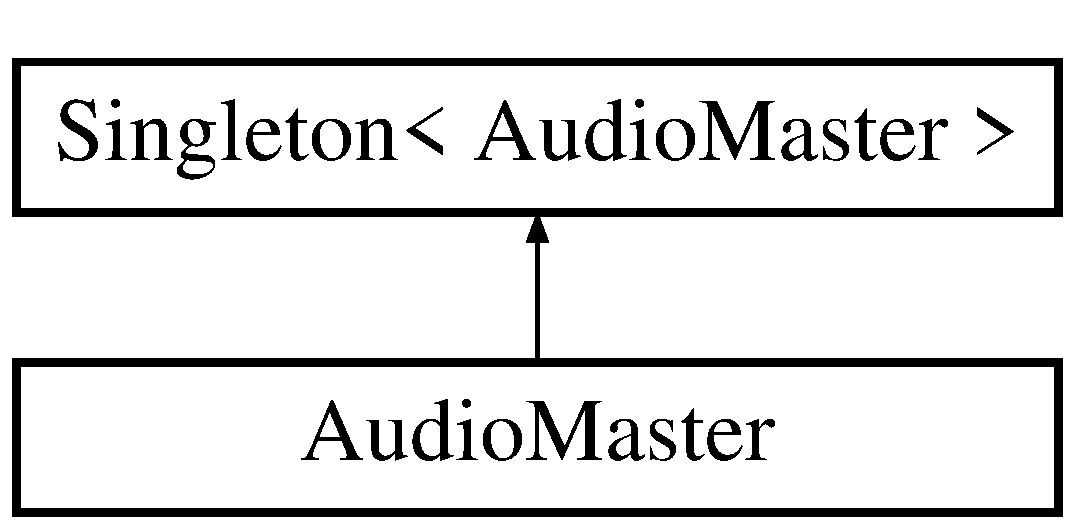
\includegraphics[height=2.000000cm]{class_d3_d11_1_1_sound_1_1_audio_master}
\end{center}
\end{figure}
\subsection*{公開メンバ関数}
\begin{DoxyCompactItemize}
\item 
\hyperlink{class_d3_d11_1_1_sound_1_1_audio_master_ac052375f8aaaff706b536d84234181af}{$\sim$\+Audio\+Master} ()\hypertarget{class_d3_d11_1_1_sound_1_1_audio_master_ac052375f8aaaff706b536d84234181af}{}\label{class_d3_d11_1_1_sound_1_1_audio_master_ac052375f8aaaff706b536d84234181af}

\begin{DoxyCompactList}\small\item\em デストラクタ \end{DoxyCompactList}\item 
H\+R\+E\+S\+U\+LT \hyperlink{class_d3_d11_1_1_sound_1_1_audio_master_a81109341187e54cc3585f29a1306ca50}{Initialize} ()
\item 
void {\bfseries Finalize} ()\hypertarget{class_d3_d11_1_1_sound_1_1_audio_master_a8fee61d7a783cade1a3d07fe86284d27}{}\label{class_d3_d11_1_1_sound_1_1_audio_master_a8fee61d7a783cade1a3d07fe86284d27}

\item 
I\+X\+Audio2 $\ast$ {\bfseries Get\+X\+Audio2} ()\hypertarget{class_d3_d11_1_1_sound_1_1_audio_master_a3cdb0063c2593b2f7639db7a9a724fab}{}\label{class_d3_d11_1_1_sound_1_1_audio_master_a3cdb0063c2593b2f7639db7a9a724fab}

\item 
I\+X\+Audio2\+Mastering\+Voice $\ast$ {\bfseries Get\+Master\+Voice} ()\hypertarget{class_d3_d11_1_1_sound_1_1_audio_master_a608d3dee26595f2a6ee1694e06259a16}{}\label{class_d3_d11_1_1_sound_1_1_audio_master_a608d3dee26595f2a6ee1694e06259a16}

\end{DoxyCompactItemize}
\subsection*{非公開メンバ関数}
\begin{DoxyCompactItemize}
\item 
\hyperlink{class_d3_d11_1_1_sound_1_1_audio_master_a88a023f4855786ba194f94086e7dedcf}{Audio\+Master} ()\hypertarget{class_d3_d11_1_1_sound_1_1_audio_master_a88a023f4855786ba194f94086e7dedcf}{}\label{class_d3_d11_1_1_sound_1_1_audio_master_a88a023f4855786ba194f94086e7dedcf}

\begin{DoxyCompactList}\small\item\em コンストラクタ \end{DoxyCompactList}\end{DoxyCompactItemize}
\subsection*{非公開変数類}
\begin{DoxyCompactItemize}
\item 
I\+X\+Audio2 $\ast$ \hyperlink{class_d3_d11_1_1_sound_1_1_audio_master_a52b9a0c3a04bc541f3eed2b0ca8263ee}{m\+\_\+p\+X\+Audio2}
\item 
I\+X\+Audio2\+Mastering\+Voice $\ast$ \hyperlink{class_d3_d11_1_1_sound_1_1_audio_master_afcd3967aaff9b5b5d845d1af09173b48}{m\+\_\+p\+Mastering\+Voice}
\end{DoxyCompactItemize}
\subsection*{フレンド}
\begin{DoxyCompactItemize}
\item 
class \hyperlink{class_d3_d11_1_1_sound_1_1_audio_master_a1f496f9283cb43702c06608d38dc22d2}{Singleton$<$ Audio\+Master $>$}\hypertarget{class_d3_d11_1_1_sound_1_1_audio_master_a1f496f9283cb43702c06608d38dc22d2}{}\label{class_d3_d11_1_1_sound_1_1_audio_master_a1f496f9283cb43702c06608d38dc22d2}

\begin{DoxyCompactList}\small\item\em シングルトンデザインパターンのテンプレート継承 \end{DoxyCompactList}\end{DoxyCompactItemize}
\subsection*{その他の継承メンバ}


\subsection{関数詳解}
\index{D3\+D11\+::\+Sound\+::\+Audio\+Master@{D3\+D11\+::\+Sound\+::\+Audio\+Master}!Initialize@{Initialize}}
\index{Initialize@{Initialize}!D3\+D11\+::\+Sound\+::\+Audio\+Master@{D3\+D11\+::\+Sound\+::\+Audio\+Master}}
\subsubsection[{\texorpdfstring{Initialize()}{Initialize()}}]{\setlength{\rightskip}{0pt plus 5cm}H\+R\+E\+S\+U\+LT Initialize (
\begin{DoxyParamCaption}
{}
\end{DoxyParamCaption}
)}\hypertarget{class_d3_d11_1_1_sound_1_1_audio_master_a81109341187e54cc3585f29a1306ca50}{}\label{class_d3_d11_1_1_sound_1_1_audio_master_a81109341187e54cc3585f29a1306ca50}
C\+O\+Mライブラリの初期化

X\+Audio2オブジェクト生成

Mastering\+Voiceオブジェクト生成 

\subsection{メンバ詳解}
\index{D3\+D11\+::\+Sound\+::\+Audio\+Master@{D3\+D11\+::\+Sound\+::\+Audio\+Master}!m\+\_\+p\+Mastering\+Voice@{m\+\_\+p\+Mastering\+Voice}}
\index{m\+\_\+p\+Mastering\+Voice@{m\+\_\+p\+Mastering\+Voice}!D3\+D11\+::\+Sound\+::\+Audio\+Master@{D3\+D11\+::\+Sound\+::\+Audio\+Master}}
\subsubsection[{\texorpdfstring{m\+\_\+p\+Mastering\+Voice}{m_pMasteringVoice}}]{\setlength{\rightskip}{0pt plus 5cm}I\+X\+Audio2\+Mastering\+Voice$\ast$ m\+\_\+p\+Mastering\+Voice\hspace{0.3cm}{\ttfamily [private]}}\hypertarget{class_d3_d11_1_1_sound_1_1_audio_master_afcd3967aaff9b5b5d845d1af09173b48}{}\label{class_d3_d11_1_1_sound_1_1_audio_master_afcd3967aaff9b5b5d845d1af09173b48}
マスタリングボイス \index{D3\+D11\+::\+Sound\+::\+Audio\+Master@{D3\+D11\+::\+Sound\+::\+Audio\+Master}!m\+\_\+p\+X\+Audio2@{m\+\_\+p\+X\+Audio2}}
\index{m\+\_\+p\+X\+Audio2@{m\+\_\+p\+X\+Audio2}!D3\+D11\+::\+Sound\+::\+Audio\+Master@{D3\+D11\+::\+Sound\+::\+Audio\+Master}}
\subsubsection[{\texorpdfstring{m\+\_\+p\+X\+Audio2}{m_pXAudio2}}]{\setlength{\rightskip}{0pt plus 5cm}I\+X\+Audio2$\ast$ m\+\_\+p\+X\+Audio2\hspace{0.3cm}{\ttfamily [private]}}\hypertarget{class_d3_d11_1_1_sound_1_1_audio_master_a52b9a0c3a04bc541f3eed2b0ca8263ee}{}\label{class_d3_d11_1_1_sound_1_1_audio_master_a52b9a0c3a04bc541f3eed2b0ca8263ee}
オーディオ 

このクラス詳解は次のファイルから抽出されました\+:\begin{DoxyCompactItemize}
\item 
C\+:/\+Users/yuuki/\+Desktop/\+Doxygen\+\_\+lib\+\_\+source/include/Audio\+Master.\+h\item 
C\+:/\+Users/yuuki/\+Desktop/\+Doxygen\+\_\+lib\+\_\+source/include/Audio\+Master.\+cpp\end{DoxyCompactItemize}

\hypertarget{class_camera}{}\section{Camera クラス}
\label{class_camera}\index{Camera@{Camera}}
Camera の継承関係図\begin{figure}[H]
\begin{center}
\leavevmode
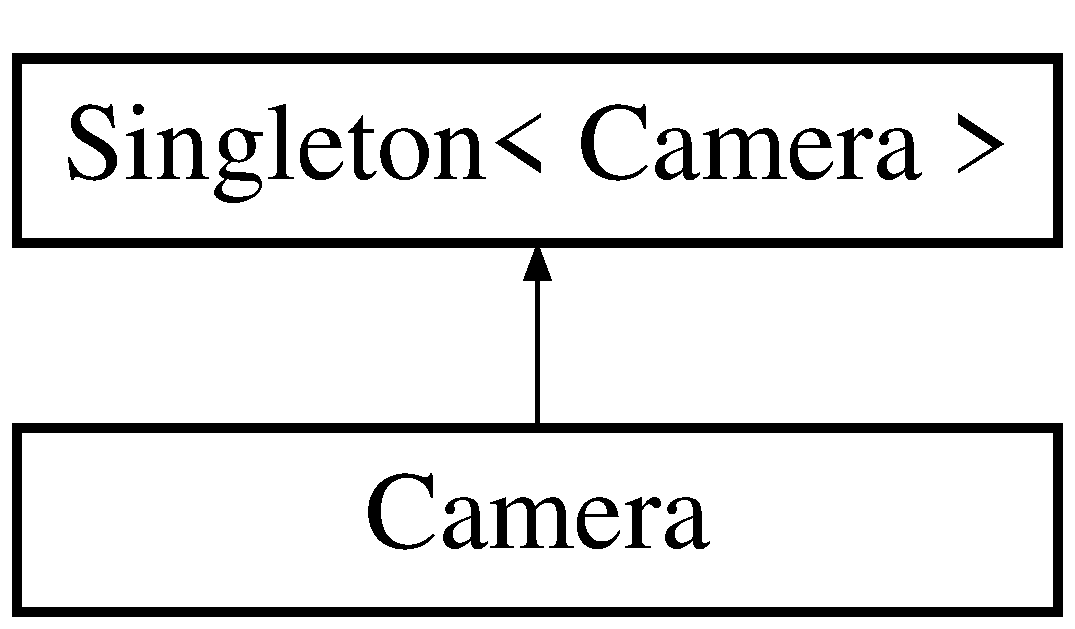
\includegraphics[height=2.000000cm]{class_camera}
\end{center}
\end{figure}
\subsection*{公開メンバ関数}
\begin{DoxyCompactItemize}
\item 
\hyperlink{class_camera_ab921e886e6f14e117eb8099ccb0a3775}{$\sim$\+Camera} ()\hypertarget{class_camera_ab921e886e6f14e117eb8099ccb0a3775}{}\label{class_camera_ab921e886e6f14e117eb8099ccb0a3775}

\begin{DoxyCompactList}\small\item\em デストラクタ \end{DoxyCompactList}\item 
void \hyperlink{class_camera_a6c93dc4a99a7b828fe37352e756e8df0}{Initialize} (Direct\+X\+::\+X\+M\+F\+L\+O\+A\+T3 eye\+Pt, Direct\+X\+::\+X\+M\+F\+L\+O\+A\+T3 look\+Pt=\{0.\+0f, 0.\+0f, 0.\+0f\}, Direct\+X\+::\+X\+M\+F\+L\+O\+A\+T3 up\+Vec=c\+\_\+\+Up\+Vector)
\begin{DoxyCompactList}\small\item\em 初期化  引数からビュー行列とプロジェクション行列を生成 \end{DoxyCompactList}\item 
Direct\+X\+::\+X\+M\+M\+A\+T\+R\+IX {\bfseries Get\+View\+Matrix} () const \hypertarget{class_camera_ac52f3bff4cb1522f3b5c5046cf69003f}{}\label{class_camera_ac52f3bff4cb1522f3b5c5046cf69003f}

\item 
Direct\+X\+::\+X\+M\+M\+A\+T\+R\+IX {\bfseries Get\+Proj\+Matrix} () const \hypertarget{class_camera_a548bbd779fcad1c6ba5bd12dabf92560}{}\label{class_camera_a548bbd779fcad1c6ba5bd12dabf92560}

\item 
Direct\+X\+::\+X\+M\+F\+L\+O\+A\+T3 \hyperlink{class_camera_af17532083692430478b8fd5006f30f0d}{Get\+Eye\+Pt} () const 
\item 
Direct\+X\+::\+X\+M\+F\+L\+O\+A\+T3 \hyperlink{class_camera_aa387eb16c079b628eb624e44467bf759}{Get\+Look\+At\+Pt} () const 
\item 
void {\bfseries Set\+Field\+Of\+View} (float fov)\hypertarget{class_camera_ab4c76305c15469fbe4eb04a493bc7b8a}{}\label{class_camera_ab4c76305c15469fbe4eb04a493bc7b8a}

\item 
void {\bfseries Set\+Near\+Clip} (float near\+Clip)\hypertarget{class_camera_a3e28bf6a3f046b81b863e23b967db7a2}{}\label{class_camera_a3e28bf6a3f046b81b863e23b967db7a2}

\item 
void {\bfseries Set\+Far\+Clip} (float far\+Clip)\hypertarget{class_camera_aecdc7fb7d7e3c7469b8e28d845a35b68}{}\label{class_camera_aecdc7fb7d7e3c7469b8e28d845a35b68}

\end{DoxyCompactItemize}
\subsection*{静的公開変数類}
\begin{DoxyCompactItemize}
\item 
static const double \hyperlink{class_camera_a54764981cc23a98b371bc5fc12d4e50e}{c\+\_\+\+Pi} = 3.\+14159265358979323846
\item 
static const float \hyperlink{class_camera_a51712c894e0df64215aae12dc97985d3}{c\+\_\+\+Field\+Of\+View} = static\+\_\+cast$<$float$>$(\hyperlink{class_camera_a54764981cc23a98b371bc5fc12d4e50e}{Camera\+::c\+\_\+\+Pi}) / 4.\+0f
\item 
static const float \hyperlink{class_camera_aa6af11ef8a84601a16811a8ef6d60fb1}{c\+\_\+\+Near\+Clip} = 0.\+1f
\item 
static const float \hyperlink{class_camera_aa5db6879f82c2538b7bfa2ae6b9e5656}{c\+\_\+\+Far\+Clip} = 100.\+0f
\item 
static const Direct\+X\+::\+X\+M\+F\+L\+O\+A\+T3 \hyperlink{class_camera_adf00fed6aca14c9362356375d267251b}{c\+\_\+\+Up\+Vector} = \{ 0.\+0f,1.\+0f,0.\+0f \}
\end{DoxyCompactItemize}
\subsection*{非公開メンバ関数}
\begin{DoxyCompactItemize}
\item 
\hyperlink{class_camera_aa3f3efcb2fcc75de885df29041103cd2}{Camera} ()
\begin{DoxyCompactList}\small\item\em コンストラクタ \end{DoxyCompactList}\end{DoxyCompactItemize}
\subsection*{非公開変数類}
\begin{DoxyCompactItemize}
\item 
float \hyperlink{class_camera_a61ed8246ec6d6d78b046d88f3f5b8bc0}{m\+\_\+\+Field\+Of\+View}
\item 
float \hyperlink{class_camera_a4bea0bad40f6b75b9c5eb19801a684a7}{m\+\_\+\+Near\+Clip}
\item 
float \hyperlink{class_camera_a803e5e33c136572ec2c31b221d2ce67f}{m\+\_\+\+Far\+Clip}
\item 
Direct\+X\+::\+X\+M\+V\+E\+C\+T\+OR \hyperlink{class_camera_a80c72afef85ca175279420cce520370d}{m\+\_\+\+Eye\+Pt}
\item 
Direct\+X\+::\+X\+M\+V\+E\+C\+T\+OR \hyperlink{class_camera_ab9dac33a4cb297f8ecdd55444df9a926}{m\+\_\+\+Look\+At\+Pt}
\item 
Direct\+X\+::\+X\+M\+V\+E\+C\+T\+OR \hyperlink{class_camera_ac1e1df300cece76a2d49ee2a1d678301}{m\+\_\+\+Up\+Vec}
\item 
Direct\+X\+::\+X\+M\+M\+A\+T\+R\+IX \hyperlink{class_camera_a06ae0945a26221c132c14896d09d1a3b}{m\+\_\+\+View\+Mat}
\item 
Direct\+X\+::\+X\+M\+M\+A\+T\+R\+IX \hyperlink{class_camera_afb229fa24074664a441b129fef4cce87}{m\+\_\+\+Proj\+Mat}
\end{DoxyCompactItemize}
\subsection*{フレンド}
\begin{DoxyCompactItemize}
\item 
class \hyperlink{class_camera_a6f66ad73633ee0655fdb0e0468c1086a}{Singleton$<$ Camera $>$}\hypertarget{class_camera_a6f66ad73633ee0655fdb0e0468c1086a}{}\label{class_camera_a6f66ad73633ee0655fdb0e0468c1086a}

\begin{DoxyCompactList}\small\item\em シングルトンデザインパターンのテンプレート継承 \end{DoxyCompactList}\end{DoxyCompactItemize}
\subsection*{その他の継承メンバ}


\subsection{構築子と解体子}
\index{Camera@{Camera}!Camera@{Camera}}
\index{Camera@{Camera}!Camera@{Camera}}
\subsubsection[{\texorpdfstring{Camera()}{Camera()}}]{\setlength{\rightskip}{0pt plus 5cm}{\bf Camera} (
\begin{DoxyParamCaption}
{}
\end{DoxyParamCaption}
)\hspace{0.3cm}{\ttfamily [private]}}\hypertarget{class_camera_aa3f3efcb2fcc75de885df29041103cd2}{}\label{class_camera_aa3f3efcb2fcc75de885df29041103cd2}


コンストラクタ 

デフォルト設定スコープ

行列の生成 

\subsection{関数詳解}
\index{Camera@{Camera}!Get\+Eye\+Pt@{Get\+Eye\+Pt}}
\index{Get\+Eye\+Pt@{Get\+Eye\+Pt}!Camera@{Camera}}
\subsubsection[{\texorpdfstring{Get\+Eye\+Pt() const }{GetEyePt() const }}]{\setlength{\rightskip}{0pt plus 5cm}Direct\+X\+::\+X\+M\+F\+L\+O\+A\+T3 Get\+Eye\+Pt (
\begin{DoxyParamCaption}
{}
\end{DoxyParamCaption}
) const}\hypertarget{class_camera_af17532083692430478b8fd5006f30f0d}{}\label{class_camera_af17532083692430478b8fd5006f30f0d}
V\+E\+C\+T\+O\+R型を\+F\+L\+O\+A\+T3に変換 \index{Camera@{Camera}!Get\+Look\+At\+Pt@{Get\+Look\+At\+Pt}}
\index{Get\+Look\+At\+Pt@{Get\+Look\+At\+Pt}!Camera@{Camera}}
\subsubsection[{\texorpdfstring{Get\+Look\+At\+Pt() const }{GetLookAtPt() const }}]{\setlength{\rightskip}{0pt plus 5cm}Direct\+X\+::\+X\+M\+F\+L\+O\+A\+T3 Get\+Look\+At\+Pt (
\begin{DoxyParamCaption}
{}
\end{DoxyParamCaption}
) const}\hypertarget{class_camera_aa387eb16c079b628eb624e44467bf759}{}\label{class_camera_aa387eb16c079b628eb624e44467bf759}
V\+E\+C\+T\+O\+R型を\+F\+L\+O\+A\+T3に変換 \index{Camera@{Camera}!Initialize@{Initialize}}
\index{Initialize@{Initialize}!Camera@{Camera}}
\subsubsection[{\texorpdfstring{Initialize(\+Direct\+X\+::\+X\+M\+F\+L\+O\+A\+T3 eye\+Pt, Direct\+X\+::\+X\+M\+F\+L\+O\+A\+T3 look\+Pt=\lcurly{}0.\+0f, 0.\+0f, 0.\+0f\rcurly{}, Direct\+X\+::\+X\+M\+F\+L\+O\+A\+T3 up\+Vec=c\+\_\+\+Up\+Vector)}{Initialize(DirectX::XMFLOAT3 eyePt, DirectX::XMFLOAT3 lookPt=\{0.0f, 0.0f, 0.0f\}, DirectX::XMFLOAT3 upVec=c_UpVector)}}]{\setlength{\rightskip}{0pt plus 5cm}void Initialize (
\begin{DoxyParamCaption}
\item[{Direct\+X\+::\+X\+M\+F\+L\+O\+A\+T3}]{eye\+Pt, }
\item[{Direct\+X\+::\+X\+M\+F\+L\+O\+A\+T3}]{look\+Pt = {\ttfamily \{~0.0f,0.0f,0.0f~\}}, }
\item[{Direct\+X\+::\+X\+M\+F\+L\+O\+A\+T3}]{up\+Vec = {\ttfamily {\bf c\+\_\+\+Up\+Vector}}}
\end{DoxyParamCaption}
)}\hypertarget{class_camera_a6c93dc4a99a7b828fe37352e756e8df0}{}\label{class_camera_a6c93dc4a99a7b828fe37352e756e8df0}


初期化  引数からビュー行列とプロジェクション行列を生成 


\begin{DoxyParams}[1]{引数}
\mbox{\tt in}  & {\em 視点位置} & \\
\hline
\mbox{\tt in}  & {\em 注視点} & \\
\hline
\mbox{\tt in}  & {\em 上向きベクトル} & \\
\hline
\end{DoxyParams}
F\+L\+O\+A\+T3を\+V\+E\+C\+T\+O\+R型に変換

ビュー行列

$<$ 視点位置

$<$ 注視点

$<$ 上向き方向

プロジェクション行列

$<$ 視野角

$<$ アスペクト比

$<$ クリッピング距離\+:近

$<$ クリッピング距離\+:遠 

\subsection{メンバ詳解}
\index{Camera@{Camera}!c\+\_\+\+Far\+Clip@{c\+\_\+\+Far\+Clip}}
\index{c\+\_\+\+Far\+Clip@{c\+\_\+\+Far\+Clip}!Camera@{Camera}}
\subsubsection[{\texorpdfstring{c\+\_\+\+Far\+Clip}{c_FarClip}}]{\setlength{\rightskip}{0pt plus 5cm}const float c\+\_\+\+Far\+Clip = 100.\+0f\hspace{0.3cm}{\ttfamily [static]}}\hypertarget{class_camera_aa5db6879f82c2538b7bfa2ae6b9e5656}{}\label{class_camera_aa5db6879f82c2538b7bfa2ae6b9e5656}
デフォルトクリッピング距離\+:遠

デフォルトのクリッピング距離\+:遠 \index{Camera@{Camera}!c\+\_\+\+Field\+Of\+View@{c\+\_\+\+Field\+Of\+View}}
\index{c\+\_\+\+Field\+Of\+View@{c\+\_\+\+Field\+Of\+View}!Camera@{Camera}}
\subsubsection[{\texorpdfstring{c\+\_\+\+Field\+Of\+View}{c_FieldOfView}}]{\setlength{\rightskip}{0pt plus 5cm}const float c\+\_\+\+Field\+Of\+View = static\+\_\+cast$<$float$>$({\bf Camera\+::c\+\_\+\+Pi}) / 4.\+0f\hspace{0.3cm}{\ttfamily [static]}}\hypertarget{class_camera_a51712c894e0df64215aae12dc97985d3}{}\label{class_camera_a51712c894e0df64215aae12dc97985d3}
画角

デフォルトの視野角(45度) \index{Camera@{Camera}!c\+\_\+\+Near\+Clip@{c\+\_\+\+Near\+Clip}}
\index{c\+\_\+\+Near\+Clip@{c\+\_\+\+Near\+Clip}!Camera@{Camera}}
\subsubsection[{\texorpdfstring{c\+\_\+\+Near\+Clip}{c_NearClip}}]{\setlength{\rightskip}{0pt plus 5cm}const float c\+\_\+\+Near\+Clip = 0.\+1f\hspace{0.3cm}{\ttfamily [static]}}\hypertarget{class_camera_aa6af11ef8a84601a16811a8ef6d60fb1}{}\label{class_camera_aa6af11ef8a84601a16811a8ef6d60fb1}
デフォルトクリッピング距離\+:近

デフォルトのクリッピング距離\+:近 \index{Camera@{Camera}!c\+\_\+\+Pi@{c\+\_\+\+Pi}}
\index{c\+\_\+\+Pi@{c\+\_\+\+Pi}!Camera@{Camera}}
\subsubsection[{\texorpdfstring{c\+\_\+\+Pi}{c_Pi}}]{\setlength{\rightskip}{0pt plus 5cm}const double c\+\_\+\+Pi = 3.\+14159265358979323846\hspace{0.3cm}{\ttfamily [static]}}\hypertarget{class_camera_a54764981cc23a98b371bc5fc12d4e50e}{}\label{class_camera_a54764981cc23a98b371bc5fc12d4e50e}
円周率π

円周率π ※\+D3\+D\+X\+\_\+\+P\+Iと同値 \index{Camera@{Camera}!c\+\_\+\+Up\+Vector@{c\+\_\+\+Up\+Vector}}
\index{c\+\_\+\+Up\+Vector@{c\+\_\+\+Up\+Vector}!Camera@{Camera}}
\subsubsection[{\texorpdfstring{c\+\_\+\+Up\+Vector}{c_UpVector}}]{\setlength{\rightskip}{0pt plus 5cm}const Direct\+X\+::\+X\+M\+F\+L\+O\+A\+T3 c\+\_\+\+Up\+Vector = \{ 0.\+0f,1.\+0f,0.\+0f \}\hspace{0.3cm}{\ttfamily [static]}}\hypertarget{class_camera_adf00fed6aca14c9362356375d267251b}{}\label{class_camera_adf00fed6aca14c9362356375d267251b}
デフォルトの上向きベクトル \index{Camera@{Camera}!m\+\_\+\+Eye\+Pt@{m\+\_\+\+Eye\+Pt}}
\index{m\+\_\+\+Eye\+Pt@{m\+\_\+\+Eye\+Pt}!Camera@{Camera}}
\subsubsection[{\texorpdfstring{m\+\_\+\+Eye\+Pt}{m_EyePt}}]{\setlength{\rightskip}{0pt plus 5cm}Direct\+X\+::\+X\+M\+V\+E\+C\+T\+OR m\+\_\+\+Eye\+Pt\hspace{0.3cm}{\ttfamily [private]}}\hypertarget{class_camera_a80c72afef85ca175279420cce520370d}{}\label{class_camera_a80c72afef85ca175279420cce520370d}
視点位置 \index{Camera@{Camera}!m\+\_\+\+Far\+Clip@{m\+\_\+\+Far\+Clip}}
\index{m\+\_\+\+Far\+Clip@{m\+\_\+\+Far\+Clip}!Camera@{Camera}}
\subsubsection[{\texorpdfstring{m\+\_\+\+Far\+Clip}{m_FarClip}}]{\setlength{\rightskip}{0pt plus 5cm}float m\+\_\+\+Far\+Clip\hspace{0.3cm}{\ttfamily [private]}}\hypertarget{class_camera_a803e5e33c136572ec2c31b221d2ce67f}{}\label{class_camera_a803e5e33c136572ec2c31b221d2ce67f}
デフォルトのクリッピング距離\+:遠 \index{Camera@{Camera}!m\+\_\+\+Field\+Of\+View@{m\+\_\+\+Field\+Of\+View}}
\index{m\+\_\+\+Field\+Of\+View@{m\+\_\+\+Field\+Of\+View}!Camera@{Camera}}
\subsubsection[{\texorpdfstring{m\+\_\+\+Field\+Of\+View}{m_FieldOfView}}]{\setlength{\rightskip}{0pt plus 5cm}float m\+\_\+\+Field\+Of\+View\hspace{0.3cm}{\ttfamily [private]}}\hypertarget{class_camera_a61ed8246ec6d6d78b046d88f3f5b8bc0}{}\label{class_camera_a61ed8246ec6d6d78b046d88f3f5b8bc0}
変数 視野角 \index{Camera@{Camera}!m\+\_\+\+Look\+At\+Pt@{m\+\_\+\+Look\+At\+Pt}}
\index{m\+\_\+\+Look\+At\+Pt@{m\+\_\+\+Look\+At\+Pt}!Camera@{Camera}}
\subsubsection[{\texorpdfstring{m\+\_\+\+Look\+At\+Pt}{m_LookAtPt}}]{\setlength{\rightskip}{0pt plus 5cm}Direct\+X\+::\+X\+M\+V\+E\+C\+T\+OR m\+\_\+\+Look\+At\+Pt\hspace{0.3cm}{\ttfamily [private]}}\hypertarget{class_camera_ab9dac33a4cb297f8ecdd55444df9a926}{}\label{class_camera_ab9dac33a4cb297f8ecdd55444df9a926}
注視点 \index{Camera@{Camera}!m\+\_\+\+Near\+Clip@{m\+\_\+\+Near\+Clip}}
\index{m\+\_\+\+Near\+Clip@{m\+\_\+\+Near\+Clip}!Camera@{Camera}}
\subsubsection[{\texorpdfstring{m\+\_\+\+Near\+Clip}{m_NearClip}}]{\setlength{\rightskip}{0pt plus 5cm}float m\+\_\+\+Near\+Clip\hspace{0.3cm}{\ttfamily [private]}}\hypertarget{class_camera_a4bea0bad40f6b75b9c5eb19801a684a7}{}\label{class_camera_a4bea0bad40f6b75b9c5eb19801a684a7}
デフォルトのクリッピング距離\+:近 \index{Camera@{Camera}!m\+\_\+\+Proj\+Mat@{m\+\_\+\+Proj\+Mat}}
\index{m\+\_\+\+Proj\+Mat@{m\+\_\+\+Proj\+Mat}!Camera@{Camera}}
\subsubsection[{\texorpdfstring{m\+\_\+\+Proj\+Mat}{m_ProjMat}}]{\setlength{\rightskip}{0pt plus 5cm}Direct\+X\+::\+X\+M\+M\+A\+T\+R\+IX m\+\_\+\+Proj\+Mat\hspace{0.3cm}{\ttfamily [private]}}\hypertarget{class_camera_afb229fa24074664a441b129fef4cce87}{}\label{class_camera_afb229fa24074664a441b129fef4cce87}
プロジェクション行列 \index{Camera@{Camera}!m\+\_\+\+Up\+Vec@{m\+\_\+\+Up\+Vec}}
\index{m\+\_\+\+Up\+Vec@{m\+\_\+\+Up\+Vec}!Camera@{Camera}}
\subsubsection[{\texorpdfstring{m\+\_\+\+Up\+Vec}{m_UpVec}}]{\setlength{\rightskip}{0pt plus 5cm}Direct\+X\+::\+X\+M\+V\+E\+C\+T\+OR m\+\_\+\+Up\+Vec\hspace{0.3cm}{\ttfamily [private]}}\hypertarget{class_camera_ac1e1df300cece76a2d49ee2a1d678301}{}\label{class_camera_ac1e1df300cece76a2d49ee2a1d678301}
上向きベクトル \index{Camera@{Camera}!m\+\_\+\+View\+Mat@{m\+\_\+\+View\+Mat}}
\index{m\+\_\+\+View\+Mat@{m\+\_\+\+View\+Mat}!Camera@{Camera}}
\subsubsection[{\texorpdfstring{m\+\_\+\+View\+Mat}{m_ViewMat}}]{\setlength{\rightskip}{0pt plus 5cm}Direct\+X\+::\+X\+M\+M\+A\+T\+R\+IX m\+\_\+\+View\+Mat\hspace{0.3cm}{\ttfamily [private]}}\hypertarget{class_camera_a06ae0945a26221c132c14896d09d1a3b}{}\label{class_camera_a06ae0945a26221c132c14896d09d1a3b}
ビュー行列 

このクラス詳解は次のファイルから抽出されました\+:\begin{DoxyCompactItemize}
\item 
C\+:/\+Users/yuuki/\+Desktop/\+Doxygen\+\_\+lib\+\_\+source/include/Camera.\+h\item 
C\+:/\+Users/yuuki/\+Desktop/\+Doxygen\+\_\+lib\+\_\+source/include/Camera.\+cpp\end{DoxyCompactItemize}

\hypertarget{class_color}{}\section{Color クラス}
\label{class_color}\index{Color@{Color}}


カラークラス  




{\ttfamily \#include $<$Color.\+h$>$}

\subsection*{公開メンバ関数}
\begin{DoxyCompactItemize}
\item 
\hyperlink{class_color_a1589b83974b42a2f3315624f14c3c92c}{Color} ()
\begin{DoxyCompactList}\small\item\em コンストラクタ \end{DoxyCompactList}\item 
\hyperlink{class_color_a77f0f61ad9bf82456a26bc055d5bb59d}{Color} (\hyperlink{class_color}{Color} \&\&color)
\begin{DoxyCompactList}\small\item\em 引数付きコンストラクタ \end{DoxyCompactList}\item 
\hyperlink{class_color_a1ad2131f9b8ad8743c40f82e557f12e3}{Color} (float r, float g, float b, float a=1.\+0f)
\begin{DoxyCompactList}\small\item\em 引数付きコンストラクタ \end{DoxyCompactList}\item 
\hyperlink{class_color_a0839ee606516f40273da5dcb0f1e85ae}{Color} (Direct\+X\+::\+X\+M\+F\+L\+O\+A\+T4 color)
\begin{DoxyCompactList}\small\item\em 引数付きコンストラクタ \end{DoxyCompactList}\item 
\hyperlink{class_color_a87ba96c77c896b3c568889338bf92444}{$\sim$\+Color} ()\hypertarget{class_color_a87ba96c77c896b3c568889338bf92444}{}\label{class_color_a87ba96c77c896b3c568889338bf92444}

\begin{DoxyCompactList}\small\item\em デストラクタ  空デストラクタ \end{DoxyCompactList}\item 
Direct\+X\+::\+X\+M\+F\+L\+O\+A\+T3 {\bfseries Get\+R\+GB} () const \hypertarget{class_color_a868cbbf6288dffa5b79861a8eadbc7e9}{}\label{class_color_a868cbbf6288dffa5b79861a8eadbc7e9}

\item 
Direct\+X\+::\+X\+M\+F\+L\+O\+A\+T4 {\bfseries Get\+R\+G\+BA} () const \hypertarget{class_color_a337d782eb5ae4dcd7b2946ce11b3e9c5}{}\label{class_color_a337d782eb5ae4dcd7b2946ce11b3e9c5}

\item 
{\bfseries Property\+Alias} (x, r, float)\hypertarget{class_color_a7aae39e182538b2d949d46e458271aeb}{}\label{class_color_a7aae39e182538b2d949d46e458271aeb}

\item 
{\bfseries Property\+Alias} (y, g, float)\hypertarget{class_color_ad99cd8a5492be2728592b0498994f4a3}{}\label{class_color_ad99cd8a5492be2728592b0498994f4a3}

\item 
{\bfseries Property\+Alias} (z, b, float)\hypertarget{class_color_ae61953d5aa2aaaa33d08f2704cef2fe1}{}\label{class_color_ae61953d5aa2aaaa33d08f2704cef2fe1}

\item 
{\bfseries Property\+Alias} (w, a, float)\hypertarget{class_color_a78543103c106d8c228ec967ce97f3b95}{}\label{class_color_a78543103c106d8c228ec967ce97f3b95}

\end{DoxyCompactItemize}
\subsection*{公開変数類}
\begin{DoxyCompactItemize}
\item 
float {\bfseries x}\hypertarget{class_color_ad0da36b2558901e21e7a30f6c227a45e}{}\label{class_color_ad0da36b2558901e21e7a30f6c227a45e}

\item 
float {\bfseries y}\hypertarget{class_color_aa4f0d3eebc3c443f9be81bf48561a217}{}\label{class_color_aa4f0d3eebc3c443f9be81bf48561a217}

\item 
float {\bfseries z}\hypertarget{class_color_af73583b1e980b0aa03f9884812e9fd4d}{}\label{class_color_af73583b1e980b0aa03f9884812e9fd4d}

\item 
float {\bfseries w}\hypertarget{class_color_a56eca241e2896b9f57a79589e76fd24b}{}\label{class_color_a56eca241e2896b9f57a79589e76fd24b}

\end{DoxyCompactItemize}


\subsection{詳解}
カラークラス 

\subsection{構築子と解体子}
\index{Color@{Color}!Color@{Color}}
\index{Color@{Color}!Color@{Color}}
\subsubsection[{\texorpdfstring{Color()}{Color()}}]{\setlength{\rightskip}{0pt plus 5cm}{\bf Color} (
\begin{DoxyParamCaption}
{}
\end{DoxyParamCaption}
)}\hypertarget{class_color_a1589b83974b42a2f3315624f14c3c92c}{}\label{class_color_a1589b83974b42a2f3315624f14c3c92c}


コンストラクタ 

コンストラクタ  デフォルト値を白にする \index{Color@{Color}!Color@{Color}}
\index{Color@{Color}!Color@{Color}}
\subsubsection[{\texorpdfstring{Color(\+Color \&\&color)}{Color(Color &&color)}}]{\setlength{\rightskip}{0pt plus 5cm}{\bf Color} (
\begin{DoxyParamCaption}
\item[{{\bf Color} \&\&}]{color}
\end{DoxyParamCaption}
)}\hypertarget{class_color_a77f0f61ad9bf82456a26bc055d5bb59d}{}\label{class_color_a77f0f61ad9bf82456a26bc055d5bb59d}


引数付きコンストラクタ 


\begin{DoxyParams}[1]{引数}
\mbox{\tt in}  & {\em 一時変数} & \\
\hline
\end{DoxyParams}
\index{Color@{Color}!Color@{Color}}
\index{Color@{Color}!Color@{Color}}
\subsubsection[{\texorpdfstring{Color(float r, float g, float b, float a=1.\+0f)}{Color(float r, float g, float b, float a=1.0f)}}]{\setlength{\rightskip}{0pt plus 5cm}{\bf Color} (
\begin{DoxyParamCaption}
\item[{float}]{r, }
\item[{float}]{g, }
\item[{float}]{b, }
\item[{float}]{a = {\ttfamily 1.0f}}
\end{DoxyParamCaption}
)}\hypertarget{class_color_a1ad2131f9b8ad8743c40f82e557f12e3}{}\label{class_color_a1ad2131f9b8ad8743c40f82e557f12e3}


引数付きコンストラクタ 


\begin{DoxyParams}[1]{引数}
\mbox{\tt in}  & {\em R(} & 0.\+0f 〜 1.\+0f ) \\
\hline
\mbox{\tt in}  & {\em G(} & 0.\+0f 〜 1.\+0f ) \\
\hline
\mbox{\tt in}  & {\em B(} & 0.\+0f 〜 1.\+0f ) \\
\hline
\mbox{\tt in}  & {\em A(} & 0.\+0f 〜 1.\+0f ) \\
\hline
\end{DoxyParams}
\index{Color@{Color}!Color@{Color}}
\index{Color@{Color}!Color@{Color}}
\subsubsection[{\texorpdfstring{Color(\+Direct\+X\+::\+X\+M\+F\+L\+O\+A\+T4 color)}{Color(DirectX::XMFLOAT4 color)}}]{\setlength{\rightskip}{0pt plus 5cm}{\bf Color} (
\begin{DoxyParamCaption}
\item[{Direct\+X\+::\+X\+M\+F\+L\+O\+A\+T4}]{color}
\end{DoxyParamCaption}
)}\hypertarget{class_color_a0839ee606516f40273da5dcb0f1e85ae}{}\label{class_color_a0839ee606516f40273da5dcb0f1e85ae}


引数付きコンストラクタ 


\begin{DoxyParams}[1]{引数}
\mbox{\tt in}  & {\em F\+L\+O\+A\+T4型からカラー型へ変換} & \\
\hline
\end{DoxyParams}


このクラス詳解は次のファイルから抽出されました\+:\begin{DoxyCompactItemize}
\item 
C\+:/\+Users/yuuki/\+Desktop/\+Doxygen\+\_\+lib\+\_\+source/include/Color.\+h\item 
C\+:/\+Users/yuuki/\+Desktop/\+Doxygen\+\_\+lib\+\_\+source/include/Color.\+cpp\end{DoxyCompactItemize}

\hypertarget{struct_d3_d11_1_1_graphic_1_1_c_o_n_s_t_a_n_t___b_u_f_f_e_r___b_a_s_e}{}\section{C\+O\+N\+S\+T\+A\+N\+T\+\_\+\+B\+U\+F\+F\+E\+R\+\_\+\+B\+A\+SE 構造体}
\label{struct_d3_d11_1_1_graphic_1_1_c_o_n_s_t_a_n_t___b_u_f_f_e_r___b_a_s_e}\index{C\+O\+N\+S\+T\+A\+N\+T\+\_\+\+B\+U\+F\+F\+E\+R\+\_\+\+B\+A\+SE@{C\+O\+N\+S\+T\+A\+N\+T\+\_\+\+B\+U\+F\+F\+E\+R\+\_\+\+B\+A\+SE}}


シェーダー側に渡すコンスタントバッファの基底構造体  




{\ttfamily \#include $<$Struct\+Shader\+Base.\+h$>$}

C\+O\+N\+S\+T\+A\+N\+T\+\_\+\+B\+U\+F\+F\+E\+R\+\_\+\+B\+A\+SE の継承関係図\begin{figure}[H]
\begin{center}
\leavevmode
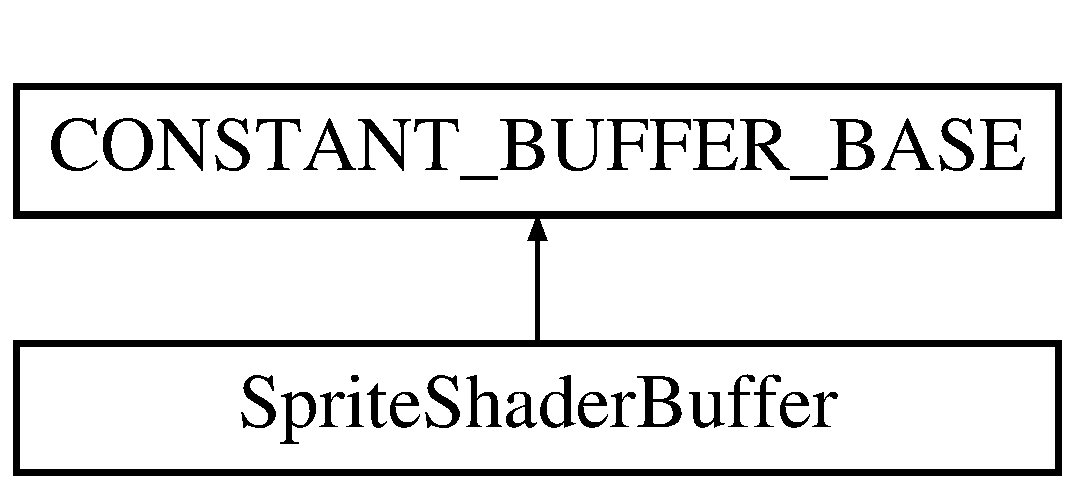
\includegraphics[height=2.000000cm]{struct_d3_d11_1_1_graphic_1_1_c_o_n_s_t_a_n_t___b_u_f_f_e_r___b_a_s_e}
\end{center}
\end{figure}
\subsection*{公開型}
\begin{DoxyCompactItemize}
\item 
{\footnotesize template$<$typename align\+Type $>$ }\\using \hyperlink{struct_d3_d11_1_1_graphic_1_1_c_o_n_s_t_a_n_t___b_u_f_f_e_r___b_a_s_e_a3443b7ba28a2ff538b5d9f5f82c02b55}{A\+L\+I\+G\+N16} = align\+Type
\end{DoxyCompactItemize}
\subsection*{公開変数類}
\begin{DoxyCompactItemize}
\item 
\hyperlink{struct_d3_d11_1_1_graphic_1_1_c_o_n_s_t_a_n_t___b_u_f_f_e_r___b_a_s_e_a3443b7ba28a2ff538b5d9f5f82c02b55}{A\+L\+I\+G\+N16}$<$ Direct\+X\+::\+X\+M\+M\+A\+T\+R\+IX $>$ \hyperlink{struct_d3_d11_1_1_graphic_1_1_c_o_n_s_t_a_n_t___b_u_f_f_e_r___b_a_s_e_aacf5d407ad2a813c4c97615ef5efb006}{m\+\_\+\+W\+VP}
\end{DoxyCompactItemize}


\subsection{詳解}
シェーダー側に渡すコンスタントバッファの基底構造体 

packマクロに変更 

\subsection{型定義メンバ詳解}
\index{D3\+D11\+::\+Graphic\+::\+C\+O\+N\+S\+T\+A\+N\+T\+\_\+\+B\+U\+F\+F\+E\+R\+\_\+\+B\+A\+SE@{D3\+D11\+::\+Graphic\+::\+C\+O\+N\+S\+T\+A\+N\+T\+\_\+\+B\+U\+F\+F\+E\+R\+\_\+\+B\+A\+SE}!A\+L\+I\+G\+N16@{A\+L\+I\+G\+N16}}
\index{A\+L\+I\+G\+N16@{A\+L\+I\+G\+N16}!D3\+D11\+::\+Graphic\+::\+C\+O\+N\+S\+T\+A\+N\+T\+\_\+\+B\+U\+F\+F\+E\+R\+\_\+\+B\+A\+SE@{D3\+D11\+::\+Graphic\+::\+C\+O\+N\+S\+T\+A\+N\+T\+\_\+\+B\+U\+F\+F\+E\+R\+\_\+\+B\+A\+SE}}
\subsubsection[{\texorpdfstring{A\+L\+I\+G\+N16}{ALIGN16}}]{\setlength{\rightskip}{0pt plus 5cm}using {\bf A\+L\+I\+G\+N16} =  align\+Type}\hypertarget{struct_d3_d11_1_1_graphic_1_1_c_o_n_s_t_a_n_t___b_u_f_f_e_r___b_a_s_e_a3443b7ba28a2ff538b5d9f5f82c02b55}{}\label{struct_d3_d11_1_1_graphic_1_1_c_o_n_s_t_a_n_t___b_u_f_f_e_r___b_a_s_e_a3443b7ba28a2ff538b5d9f5f82c02b55}
16バイト境界に型を設定するための別名 

\subsection{メンバ詳解}
\index{D3\+D11\+::\+Graphic\+::\+C\+O\+N\+S\+T\+A\+N\+T\+\_\+\+B\+U\+F\+F\+E\+R\+\_\+\+B\+A\+SE@{D3\+D11\+::\+Graphic\+::\+C\+O\+N\+S\+T\+A\+N\+T\+\_\+\+B\+U\+F\+F\+E\+R\+\_\+\+B\+A\+SE}!m\+\_\+\+W\+VP@{m\+\_\+\+W\+VP}}
\index{m\+\_\+\+W\+VP@{m\+\_\+\+W\+VP}!D3\+D11\+::\+Graphic\+::\+C\+O\+N\+S\+T\+A\+N\+T\+\_\+\+B\+U\+F\+F\+E\+R\+\_\+\+B\+A\+SE@{D3\+D11\+::\+Graphic\+::\+C\+O\+N\+S\+T\+A\+N\+T\+\_\+\+B\+U\+F\+F\+E\+R\+\_\+\+B\+A\+SE}}
\subsubsection[{\texorpdfstring{m\+\_\+\+W\+VP}{m_WVP}}]{\setlength{\rightskip}{0pt plus 5cm}{\bf A\+L\+I\+G\+N16}$<$Direct\+X\+::\+X\+M\+M\+A\+T\+R\+IX$>$ m\+\_\+\+W\+VP}\hypertarget{struct_d3_d11_1_1_graphic_1_1_c_o_n_s_t_a_n_t___b_u_f_f_e_r___b_a_s_e_aacf5d407ad2a813c4c97615ef5efb006}{}\label{struct_d3_d11_1_1_graphic_1_1_c_o_n_s_t_a_n_t___b_u_f_f_e_r___b_a_s_e_aacf5d407ad2a813c4c97615ef5efb006}
メンバの行列 

この構造体詳解は次のファイルから抽出されました\+:\begin{DoxyCompactItemize}
\item 
C\+:/\+Users/yuuki/\+Desktop/\+Doxygen\+\_\+lib\+\_\+source/include/Struct\+Shader\+Base.\+h\end{DoxyCompactItemize}

\hypertarget{class_debug}{}\section{Debug クラス}
\label{class_debug}\index{Debug@{Debug}}


デバッグ用シンボルの宣言  Releaseビルド時に有効にならないようマクロで囲む  




{\ttfamily \#include $<$Debug.\+h$>$}

\subsection*{静的公開メンバ関数}
\begin{DoxyCompactItemize}
\item 
static bool \hyperlink{class_debug_a9010a273f655a34e0383917d2108a204}{Create\+Console\+Window} ()
\item 
static void {\bfseries Destroy\+Console\+Window} ()\hypertarget{class_debug_a8e316a9c6e380131ee036b41ab080bac}{}\label{class_debug_a8e316a9c6e380131ee036b41ab080bac}

\item 
static void \hyperlink{class_debug_ae62056266b5e3ea2c0532a7740ad3368}{Disable\+Close\+Button} ()
\end{DoxyCompactItemize}
\subsection*{静的非公開変数類}
\begin{DoxyCompactItemize}
\item 
static H\+W\+ND \hyperlink{class_debug_aac93c9dce14754b224b4f30c58301a41}{m\+\_\+h\+Wnd\+Console} = nullptr
\item 
static H\+M\+E\+NU \hyperlink{class_debug_afd3dd5f72cf90cc16b3aebc01e53bcf3}{m\+\_\+h\+Menu} = nullptr
\end{DoxyCompactItemize}


\subsection{詳解}
デバッグ用シンボルの宣言  Releaseビルド時に有効にならないようマクロで囲む 

デバッグクラス 

\subsection{関数詳解}
\index{Debug@{Debug}!Create\+Console\+Window@{Create\+Console\+Window}}
\index{Create\+Console\+Window@{Create\+Console\+Window}!Debug@{Debug}}
\subsubsection[{\texorpdfstring{Create\+Console\+Window()}{CreateConsoleWindow()}}]{\setlength{\rightskip}{0pt plus 5cm}bool Create\+Console\+Window (
\begin{DoxyParamCaption}
{}
\end{DoxyParamCaption}
)\hspace{0.3cm}{\ttfamily [static]}}\hypertarget{class_debug_a9010a273f655a34e0383917d2108a204}{}\label{class_debug_a9010a273f655a34e0383917d2108a204}
コンソール作成

標準入出力に割り当てる

新たなファイルを開きストリームと結びつける

ウィンドウハンドラ取得

メニューハンドラ取得 \index{Debug@{Debug}!Disable\+Close\+Button@{Disable\+Close\+Button}}
\index{Disable\+Close\+Button@{Disable\+Close\+Button}!Debug@{Debug}}
\subsubsection[{\texorpdfstring{Disable\+Close\+Button()}{DisableCloseButton()}}]{\setlength{\rightskip}{0pt plus 5cm}void Disable\+Close\+Button (
\begin{DoxyParamCaption}
{}
\end{DoxyParamCaption}
)\hspace{0.3cm}{\ttfamily [static]}}\hypertarget{class_debug_ae62056266b5e3ea2c0532a7740ad3368}{}\label{class_debug_ae62056266b5e3ea2c0532a7740ad3368}
メニューの閉じるボタンを無効化 

\subsection{メンバ詳解}
\index{Debug@{Debug}!m\+\_\+h\+Menu@{m\+\_\+h\+Menu}}
\index{m\+\_\+h\+Menu@{m\+\_\+h\+Menu}!Debug@{Debug}}
\subsubsection[{\texorpdfstring{m\+\_\+h\+Menu}{m_hMenu}}]{\setlength{\rightskip}{0pt plus 5cm}H\+M\+E\+NU m\+\_\+h\+Menu = nullptr\hspace{0.3cm}{\ttfamily [static]}, {\ttfamily [private]}}\hypertarget{class_debug_afd3dd5f72cf90cc16b3aebc01e53bcf3}{}\label{class_debug_afd3dd5f72cf90cc16b3aebc01e53bcf3}
メニューハンドラ \index{Debug@{Debug}!m\+\_\+h\+Wnd\+Console@{m\+\_\+h\+Wnd\+Console}}
\index{m\+\_\+h\+Wnd\+Console@{m\+\_\+h\+Wnd\+Console}!Debug@{Debug}}
\subsubsection[{\texorpdfstring{m\+\_\+h\+Wnd\+Console}{m_hWndConsole}}]{\setlength{\rightskip}{0pt plus 5cm}H\+W\+ND m\+\_\+h\+Wnd\+Console = nullptr\hspace{0.3cm}{\ttfamily [static]}, {\ttfamily [private]}}\hypertarget{class_debug_aac93c9dce14754b224b4f30c58301a41}{}\label{class_debug_aac93c9dce14754b224b4f30c58301a41}
コンソールウィンドウハンドラ

静的メンバ変数の初期化と宣言 

このクラス詳解は次のファイルから抽出されました\+:\begin{DoxyCompactItemize}
\item 
C\+:/\+Users/yuuki/\+Desktop/\+Doxygen\+\_\+lib\+\_\+source/include/\hyperlink{_debug_8h}{Debug.\+h}\item 
C\+:/\+Users/yuuki/\+Desktop/\+Doxygen\+\_\+lib\+\_\+source/include/\hyperlink{_debug_8cpp}{Debug.\+cpp}\end{DoxyCompactItemize}

\hypertarget{class_d3_d11_1_1_direct3_d11}{}\section{Direct3\+D11 クラス}
\label{class_d3_d11_1_1_direct3_d11}\index{Direct3\+D11@{Direct3\+D11}}


Direct3\+D11デバイスclass.  




{\ttfamily \#include $<$Direct3\+D11.\+h$>$}

Direct3\+D11 の継承関係図\begin{figure}[H]
\begin{center}
\leavevmode
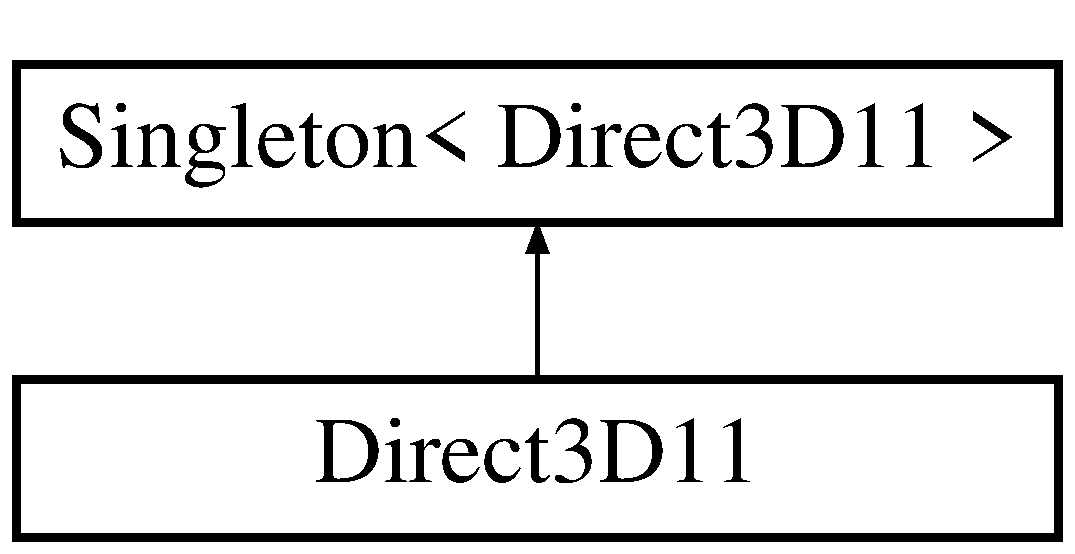
\includegraphics[height=2.000000cm]{class_d3_d11_1_1_direct3_d11}
\end{center}
\end{figure}
\subsection*{公開メンバ関数}
\begin{DoxyCompactItemize}
\item 
\hyperlink{class_d3_d11_1_1_direct3_d11_a99102e32e8ba1004955d94885322776b}{$\sim$\+Direct3\+D11} ()\hypertarget{class_d3_d11_1_1_direct3_d11_a99102e32e8ba1004955d94885322776b}{}\label{class_d3_d11_1_1_direct3_d11_a99102e32e8ba1004955d94885322776b}

\begin{DoxyCompactList}\small\item\em デストラクタ \end{DoxyCompactList}\item 
H\+R\+E\+S\+U\+LT \hyperlink{class_d3_d11_1_1_direct3_d11_a9567d2e7c0ccc19e447154f25335e006}{Initialize} (H\+W\+ND h\+Wnd)
\item 
void {\bfseries Release} ()\hypertarget{class_d3_d11_1_1_direct3_d11_a94c93747c8daa99d65c2a04c6be0748c}{}\label{class_d3_d11_1_1_direct3_d11_a94c93747c8daa99d65c2a04c6be0748c}

\item 
void \hyperlink{class_d3_d11_1_1_direct3_d11_aa71d36872f416feaa853788a7a7a7ef8}{Clear} ()
\item 
void \hyperlink{class_d3_d11_1_1_direct3_d11_a9b05a17ef5246aa3edb781748d58fd2b}{Present} ()
\item 
void \hyperlink{class_d3_d11_1_1_direct3_d11_a630f2a359e353bf01f907f1ed0efc3e4}{Report\+C\+O\+Ms} (std\+::string first\+Message=\char`\"{}\char`\"{})
\item 
I\+D3\+D11\+Device $\ast$ {\bfseries Get\+Device} () const \hypertarget{class_d3_d11_1_1_direct3_d11_a2d29a54e96836ca83181418a4d55ec28}{}\label{class_d3_d11_1_1_direct3_d11_a2d29a54e96836ca83181418a4d55ec28}

\item 
I\+D3\+D11\+Device\+Context $\ast$ {\bfseries Get\+Device\+Context} () const \hypertarget{class_d3_d11_1_1_direct3_d11_a7c867cc4d7cb092b0c17eb44704e2221}{}\label{class_d3_d11_1_1_direct3_d11_a7c867cc4d7cb092b0c17eb44704e2221}

\end{DoxyCompactItemize}
\subsection*{非公開メンバ関数}
\begin{DoxyCompactItemize}
\item 
\hyperlink{class_d3_d11_1_1_direct3_d11_aefd83bcdc7237ec876a4d4800d4e4707}{Direct3\+D11} ()\hypertarget{class_d3_d11_1_1_direct3_d11_aefd83bcdc7237ec876a4d4800d4e4707}{}\label{class_d3_d11_1_1_direct3_d11_aefd83bcdc7237ec876a4d4800d4e4707}

\begin{DoxyCompactList}\small\item\em コンストラクタ \end{DoxyCompactList}\end{DoxyCompactItemize}
\subsection*{非公開変数類}
\begin{DoxyCompactItemize}
\item 
Microsoft\+::\+W\+R\+L\+::\+Com\+Ptr$<$ I\+D3\+D11\+Device $>$ \hyperlink{class_d3_d11_1_1_direct3_d11_a76be9b3348b0abf14aaf6fc74f1c6ce8}{m\+\_\+p\+Device}
\begin{DoxyCompactList}\small\item\em メンバー変数の宣言  Com\+Ptrを使ったスマートポインタで宣言 \end{DoxyCompactList}\item 
Microsoft\+::\+W\+R\+L\+::\+Com\+Ptr$<$ I\+D3\+D11\+Device\+Context $>$ \hyperlink{class_d3_d11_1_1_direct3_d11_a96130435411c63bd3fbe61b3ea72cd1e}{m\+\_\+p\+Device\+Context}
\item 
Microsoft\+::\+W\+R\+L\+::\+Com\+Ptr$<$ I\+D\+X\+G\+I\+Swap\+Chain $>$ \hyperlink{class_d3_d11_1_1_direct3_d11_ac65621ae00fb1dc6918fad9de8777982}{m\+\_\+p\+Swap\+Chain}
\item 
Microsoft\+::\+W\+R\+L\+::\+Com\+Ptr$<$ I\+D3\+D11\+Render\+Target\+View $>$ \hyperlink{class_d3_d11_1_1_direct3_d11_a43a0f700bf837a8b14463a295aa78a0d}{m\+\_\+p\+Render\+Target\+View}
\item 
Microsoft\+::\+W\+R\+L\+::\+Com\+Ptr$<$ I\+D3\+D11\+Depth\+Stencil\+View $>$ \hyperlink{class_d3_d11_1_1_direct3_d11_aaf400f9f61eb658eafd0ca0c07bce101}{m\+\_\+p\+Depth\+Stencil\+View}
\item 
Microsoft\+::\+W\+R\+L\+::\+Com\+Ptr$<$ I\+D3\+D11\+Texture2D $>$ \hyperlink{class_d3_d11_1_1_direct3_d11_a57ba9b5b193de73e3832ed5afb20fc10}{m\+\_\+p\+Depth\+Stencil}
\item 
Microsoft\+::\+W\+R\+L\+::\+Com\+Ptr$<$ I\+D3\+D11\+Depth\+Stencil\+State $>$ \hyperlink{class_d3_d11_1_1_direct3_d11_a20316c9265ff7890678f87d99ba824c8}{m\+\_\+p\+Depth\+Stencil\+State}
\item 
Microsoft\+::\+W\+R\+L\+::\+Com\+Ptr$<$ I\+D3\+D11\+Rasterizer\+State $>$ \hyperlink{class_d3_d11_1_1_direct3_d11_a5332afbf9cb9c36f53b0c05219ed4ac0}{m\+\_\+p\+Rasterizer\+State}
\item 
Microsoft\+::\+W\+R\+L\+::\+Com\+Ptr$<$ I\+D3\+D11\+Debug $>$ \hyperlink{class_d3_d11_1_1_direct3_d11_a2322202b2972971329f77e27a6c0373b}{m\+\_\+p\+Debug}
\end{DoxyCompactItemize}
\subsection*{静的非公開変数類}
\begin{DoxyCompactItemize}
\item 
static const float \hyperlink{class_d3_d11_1_1_direct3_d11_a34ce02602072a5783535c33d2c8ed6bc}{c\+\_\+\+Clear\+Color} \mbox{[}4\mbox{]} \{ 0.\+5f,0.\+5f,1.\+5f,1.\+0f \}
\begin{DoxyCompactList}\small\item\em 描画ターゲットのクリアカラー \end{DoxyCompactList}\end{DoxyCompactItemize}
\subsection*{フレンド}
\begin{DoxyCompactItemize}
\item 
class \hyperlink{class_d3_d11_1_1_direct3_d11_a391b0c96d3c9b1128f584cb6b46cdeeb}{Singleton$<$ Direct3\+D11 $>$}\hypertarget{class_d3_d11_1_1_direct3_d11_a391b0c96d3c9b1128f584cb6b46cdeeb}{}\label{class_d3_d11_1_1_direct3_d11_a391b0c96d3c9b1128f584cb6b46cdeeb}

\begin{DoxyCompactList}\small\item\em シングルトンデザインパターンのテンプレート継承 \end{DoxyCompactList}\end{DoxyCompactItemize}
\subsection*{その他の継承メンバ}


\subsection{詳解}
Direct3\+D11デバイスclass. 

\subsection{関数詳解}
\index{D3\+D11\+::\+Direct3\+D11@{D3\+D11\+::\+Direct3\+D11}!Clear@{Clear}}
\index{Clear@{Clear}!D3\+D11\+::\+Direct3\+D11@{D3\+D11\+::\+Direct3\+D11}}
\subsubsection[{\texorpdfstring{Clear()}{Clear()}}]{\setlength{\rightskip}{0pt plus 5cm}void Clear (
\begin{DoxyParamCaption}
{}
\end{DoxyParamCaption}
)}\hypertarget{class_d3_d11_1_1_direct3_d11_aa71d36872f416feaa853788a7a7a7ef8}{}\label{class_d3_d11_1_1_direct3_d11_aa71d36872f416feaa853788a7a7a7ef8}
レンダーターゲットビューのクリア

$<$ クリアするレンダーターゲットビュー

$<$ クリアカラー

デプス・ステンシルビューのクリア

$<$ クリアするデプス・ステンシルビュー

$<$ クリアするデータの型

$<$ 深度バッファのクリア値

$<$ ステンシルバッファのクリア値 \index{D3\+D11\+::\+Direct3\+D11@{D3\+D11\+::\+Direct3\+D11}!Initialize@{Initialize}}
\index{Initialize@{Initialize}!D3\+D11\+::\+Direct3\+D11@{D3\+D11\+::\+Direct3\+D11}}
\subsubsection[{\texorpdfstring{Initialize(\+H\+W\+N\+D h\+Wnd)}{Initialize(HWND hWnd)}}]{\setlength{\rightskip}{0pt plus 5cm}H\+R\+E\+S\+U\+LT Initialize (
\begin{DoxyParamCaption}
\item[{H\+W\+ND}]{h\+Wnd}
\end{DoxyParamCaption}
)}\hypertarget{class_d3_d11_1_1_direct3_d11_a9567d2e7c0ccc19e447154f25335e006}{}\label{class_d3_d11_1_1_direct3_d11_a9567d2e7c0ccc19e447154f25335e006}
デバイスとスワップ・チェイン作成

$<$ バック・バッファ数

$<$ バック・バッファの幅

$<$ バック・バッファの高さ

$<$ フォーマット

$<$ リフレッシュ・レート(分子)

$<$ リフレッシュ・レート(分母)

スキャンライン描画モード

スケーリング・モード

$<$ バック・バッファの仕様

$<$ 関連付けるウィンドウ

アンチエイリアス処理無し

$<$ マルチ・サンプルの数

$<$ マルチ・サンプルのクオリティ

$<$ ウィンドウ・モード

$<$ スワップ・チェイン効果指定

機能レベルを指定する配列

$<$ 機能レベルを取得する変数

デバイスとスワップ・チェインの作成

$<$ 使用する\+I\+D\+X\+G\+I\+Adapter インターフェース

$<$ Direct3D 11 デバイスの種類

$<$ 使用する\+A\+PI レイヤーの指定

$<$ 機能レベルを指定する配列

$<$ 上記配列の要素数

$<$ 使用している\+S\+D\+Kのバージョン

$<$ スワップ・チェインの設定

$<$ I\+D\+X\+G\+I\+Swap\+Chain インターフェースの変数

$<$ I\+D3\+D11\+Device インターフェースの変数

$<$ 機能レベルを取得する変数

$<$ I\+D3\+D11\+Device\+Context インターフェースの変数

$<$ デバイスの作成に失敗

スワップ・チェインから最初のバックバッファを取得する

$<$ バック・バッファ番号

$<$ バッファにアクセスするインターフェース

$<$ バッファを受け取る変数

$<$ 取得失敗

レンダーターゲットビューの作成

$<$ ビューでアクセスするリソース

$<$ レンダーターゲットビューの定義

$<$ レンダーターゲットビューを受け取る変数

バック・バッファは以降使わないので解放

$<$ レンダーターゲットビューの作成に失敗

深度テクスチャ / ステンシルビュー / ステンシルステートの作成

深度 /ステンシル・ステート設定

$<$ 深度テスト有り

$<$ 書き込む

$<$ 手前の物体を描画

$<$ ステンシル・テスト無し

$<$ ステンシル書き込みマスク

$<$ ステンシル読み込みマスク

面が表を向いている場合のステンシル・テストの設定

$<$ ステンシルテストが失敗した時に実行されるステンシル処理

$<$ ステンシルテストが合格で深度テストが不合格の場合に実行される処理

$<$ ステンシルテストと深度テストの両方が合格の場合に実行されるステンシル処理

$<$ 既存のデータに対するデータの比較方法

面が裏を向いている場合のステンシル・テストの設定

$<$ ステンシルテストが失敗した時に実行されるステンシル処理

$<$ ステンシルテストが合格で深度テストが不合格の場合に実行される処理

$<$ ステンシルテストと深度テストの両方が合格の場合に実行されるステンシル処理

$<$ 既存のデータに対するデータの比較方法

深度 /ステンシル・ステート作成

$<$ 深度 /ステンシル・ステート設定情報

$<$ 作成した 深度 /ステンシル・ステートを受け取る変数

$<$ 深度 /ステンシル・ステート作成失敗

深度 /ステンシル・ステート適応

$<$ 深度 /ステンシル・ステート

$<$ ステンシル・テストで参照値

深度 / ステンシル・テクスチャの設定

$<$ 幅

$<$ 高さ

$<$ ミップマップ・レベル数

$<$ 配列サイズ

$<$ フォーマット(深度のみ)

$<$ マルチサンプリングの設定

$<$ マルチサンプリングの品質

$<$ デフォルトの仕様

$<$ 深度 / ステンシルとして使用

$<$ C\+P\+Uからはアクセスしない

$<$ その他 設定なし

深度 / ステンシル・テクスチャの作成

$<$ 作成する2\+Dテクスチャの設定

$<$ M\+S\+A\+Aを利用する場合 N\+U\+LL にする

$<$ 作成したテクスチャを受けとる変数

$<$ ステンシルテクスチャの作成に失敗

深度 / ステンシル・ビュー設定

$<$ ビューのフォーマット

$<$ リソースの種類

深度 / ステンシル・テクスチャに対しビューを作成

$<$ 深度 / ステンシル・ビューを作るテクスチャ

$<$ 深度 / ステンシル・ビューの設定

$<$ 作成したビューを受け取る変数

描画ターゲット・ビューを出力マネージャーのターゲットとして設定

$<$ 描画ターゲット数

$<$ 描画ターゲットビュー

$<$ 深度 / ステンシルビュー

ビューポートの設定

$<$ ビューポート領域の幅

$<$ ビューポート領域の高さ

$<$ ビューポート領域の深度最大値(ファー・クリッピング距離)

$<$ ビューポートの数

$<$ 設定するビューポート配列

ラスタライズ設定

$<$ 普通に描画

$<$ 両面を描画

$<$ 深度バイアス「0」

$<$ 深度クリッピング無し

$<$ シザー矩形無し

$<$ マルチサンプリング無し

$<$ ライン・アンチエイリアシング無し

ラスタライズ設定の作成

$<$ ラスタライズ設定

$<$ 設定を受け取る変数

$<$ ラスタライザーステート作成失敗

ラスタライズを設定

初期化終了 \index{D3\+D11\+::\+Direct3\+D11@{D3\+D11\+::\+Direct3\+D11}!Present@{Present}}
\index{Present@{Present}!D3\+D11\+::\+Direct3\+D11@{D3\+D11\+::\+Direct3\+D11}}
\subsubsection[{\texorpdfstring{Present()}{Present()}}]{\setlength{\rightskip}{0pt plus 5cm}void Present (
\begin{DoxyParamCaption}
{}
\end{DoxyParamCaption}
)}\hypertarget{class_d3_d11_1_1_direct3_d11_a9b05a17ef5246aa3edb781748d58fd2b}{}\label{class_d3_d11_1_1_direct3_d11_a9b05a17ef5246aa3edb781748d58fd2b}
$<$ 画面更新(D\+X\+G\+I\+\_\+\+P\+R\+E\+S\+E\+N\+T\+\_\+\+T\+E\+S\+Tだと更新は行わない) \index{D3\+D11\+::\+Direct3\+D11@{D3\+D11\+::\+Direct3\+D11}!Report\+C\+O\+Ms@{Report\+C\+O\+Ms}}
\index{Report\+C\+O\+Ms@{Report\+C\+O\+Ms}!D3\+D11\+::\+Direct3\+D11@{D3\+D11\+::\+Direct3\+D11}}
\subsubsection[{\texorpdfstring{Report\+C\+O\+Ms(std\+::string first\+Message="""")}{ReportCOMs(std::string firstMessage="")}}]{\setlength{\rightskip}{0pt plus 5cm}void Report\+C\+O\+Ms (
\begin{DoxyParamCaption}
\item[{std\+::string}]{first\+Message = {\ttfamily \char`\"{}\char`\"{}}}
\end{DoxyParamCaption}
)}\hypertarget{class_d3_d11_1_1_direct3_d11_a630f2a359e353bf01f907f1ed0efc3e4}{}\label{class_d3_d11_1_1_direct3_d11_a630f2a359e353bf01f907f1ed0efc3e4}
デバッグインターフェイスのチェック

ウィンドウに任意の文字列を表示

C\+O\+Mの生存状況を出力ウィンドウに出力 

\subsection{メンバ詳解}
\index{D3\+D11\+::\+Direct3\+D11@{D3\+D11\+::\+Direct3\+D11}!c\+\_\+\+Clear\+Color@{c\+\_\+\+Clear\+Color}}
\index{c\+\_\+\+Clear\+Color@{c\+\_\+\+Clear\+Color}!D3\+D11\+::\+Direct3\+D11@{D3\+D11\+::\+Direct3\+D11}}
\subsubsection[{\texorpdfstring{c\+\_\+\+Clear\+Color}{c_ClearColor}}]{\setlength{\rightskip}{0pt plus 5cm}c\+\_\+\+Clear\+Color \{ 0.\+5f,0.\+5f,1.\+5f,1.\+0f \}\hspace{0.3cm}{\ttfamily [static]}, {\ttfamily [private]}}\hypertarget{class_d3_d11_1_1_direct3_d11_a34ce02602072a5783535c33d2c8ed6bc}{}\label{class_d3_d11_1_1_direct3_d11_a34ce02602072a5783535c33d2c8ed6bc}


描画ターゲットのクリアカラー 

描画ターゲットクリアカラー \index{D3\+D11\+::\+Direct3\+D11@{D3\+D11\+::\+Direct3\+D11}!m\+\_\+p\+Debug@{m\+\_\+p\+Debug}}
\index{m\+\_\+p\+Debug@{m\+\_\+p\+Debug}!D3\+D11\+::\+Direct3\+D11@{D3\+D11\+::\+Direct3\+D11}}
\subsubsection[{\texorpdfstring{m\+\_\+p\+Debug}{m_pDebug}}]{\setlength{\rightskip}{0pt plus 5cm}Microsoft\+::\+W\+R\+L\+::\+Com\+Ptr$<$I\+D3\+D11\+Debug$>$ m\+\_\+p\+Debug\hspace{0.3cm}{\ttfamily [private]}}\hypertarget{class_d3_d11_1_1_direct3_d11_a2322202b2972971329f77e27a6c0373b}{}\label{class_d3_d11_1_1_direct3_d11_a2322202b2972971329f77e27a6c0373b}
デバッグ \index{D3\+D11\+::\+Direct3\+D11@{D3\+D11\+::\+Direct3\+D11}!m\+\_\+p\+Depth\+Stencil@{m\+\_\+p\+Depth\+Stencil}}
\index{m\+\_\+p\+Depth\+Stencil@{m\+\_\+p\+Depth\+Stencil}!D3\+D11\+::\+Direct3\+D11@{D3\+D11\+::\+Direct3\+D11}}
\subsubsection[{\texorpdfstring{m\+\_\+p\+Depth\+Stencil}{m_pDepthStencil}}]{\setlength{\rightskip}{0pt plus 5cm}Microsoft\+::\+W\+R\+L\+::\+Com\+Ptr$<$I\+D3\+D11\+Texture2D$>$ m\+\_\+p\+Depth\+Stencil\hspace{0.3cm}{\ttfamily [private]}}\hypertarget{class_d3_d11_1_1_direct3_d11_a57ba9b5b193de73e3832ed5afb20fc10}{}\label{class_d3_d11_1_1_direct3_d11_a57ba9b5b193de73e3832ed5afb20fc10}
デプスステンシル \index{D3\+D11\+::\+Direct3\+D11@{D3\+D11\+::\+Direct3\+D11}!m\+\_\+p\+Depth\+Stencil\+State@{m\+\_\+p\+Depth\+Stencil\+State}}
\index{m\+\_\+p\+Depth\+Stencil\+State@{m\+\_\+p\+Depth\+Stencil\+State}!D3\+D11\+::\+Direct3\+D11@{D3\+D11\+::\+Direct3\+D11}}
\subsubsection[{\texorpdfstring{m\+\_\+p\+Depth\+Stencil\+State}{m_pDepthStencilState}}]{\setlength{\rightskip}{0pt plus 5cm}Microsoft\+::\+W\+R\+L\+::\+Com\+Ptr$<$I\+D3\+D11\+Depth\+Stencil\+State$>$ m\+\_\+p\+Depth\+Stencil\+State\hspace{0.3cm}{\ttfamily [private]}}\hypertarget{class_d3_d11_1_1_direct3_d11_a20316c9265ff7890678f87d99ba824c8}{}\label{class_d3_d11_1_1_direct3_d11_a20316c9265ff7890678f87d99ba824c8}
デプスステンシルステート \index{D3\+D11\+::\+Direct3\+D11@{D3\+D11\+::\+Direct3\+D11}!m\+\_\+p\+Depth\+Stencil\+View@{m\+\_\+p\+Depth\+Stencil\+View}}
\index{m\+\_\+p\+Depth\+Stencil\+View@{m\+\_\+p\+Depth\+Stencil\+View}!D3\+D11\+::\+Direct3\+D11@{D3\+D11\+::\+Direct3\+D11}}
\subsubsection[{\texorpdfstring{m\+\_\+p\+Depth\+Stencil\+View}{m_pDepthStencilView}}]{\setlength{\rightskip}{0pt plus 5cm}Microsoft\+::\+W\+R\+L\+::\+Com\+Ptr$<$I\+D3\+D11\+Depth\+Stencil\+View$>$ m\+\_\+p\+Depth\+Stencil\+View\hspace{0.3cm}{\ttfamily [private]}}\hypertarget{class_d3_d11_1_1_direct3_d11_aaf400f9f61eb658eafd0ca0c07bce101}{}\label{class_d3_d11_1_1_direct3_d11_aaf400f9f61eb658eafd0ca0c07bce101}
デプスステンシルビュー \index{D3\+D11\+::\+Direct3\+D11@{D3\+D11\+::\+Direct3\+D11}!m\+\_\+p\+Device@{m\+\_\+p\+Device}}
\index{m\+\_\+p\+Device@{m\+\_\+p\+Device}!D3\+D11\+::\+Direct3\+D11@{D3\+D11\+::\+Direct3\+D11}}
\subsubsection[{\texorpdfstring{m\+\_\+p\+Device}{m_pDevice}}]{\setlength{\rightskip}{0pt plus 5cm}Microsoft\+::\+W\+R\+L\+::\+Com\+Ptr$<$I\+D3\+D11\+Device$>$ m\+\_\+p\+Device\hspace{0.3cm}{\ttfamily [private]}}\hypertarget{class_d3_d11_1_1_direct3_d11_a76be9b3348b0abf14aaf6fc74f1c6ce8}{}\label{class_d3_d11_1_1_direct3_d11_a76be9b3348b0abf14aaf6fc74f1c6ce8}


メンバー変数の宣言  Com\+Ptrを使ったスマートポインタで宣言 

デバイス \index{D3\+D11\+::\+Direct3\+D11@{D3\+D11\+::\+Direct3\+D11}!m\+\_\+p\+Device\+Context@{m\+\_\+p\+Device\+Context}}
\index{m\+\_\+p\+Device\+Context@{m\+\_\+p\+Device\+Context}!D3\+D11\+::\+Direct3\+D11@{D3\+D11\+::\+Direct3\+D11}}
\subsubsection[{\texorpdfstring{m\+\_\+p\+Device\+Context}{m_pDeviceContext}}]{\setlength{\rightskip}{0pt plus 5cm}Microsoft\+::\+W\+R\+L\+::\+Com\+Ptr$<$I\+D3\+D11\+Device\+Context$>$ m\+\_\+p\+Device\+Context\hspace{0.3cm}{\ttfamily [private]}}\hypertarget{class_d3_d11_1_1_direct3_d11_a96130435411c63bd3fbe61b3ea72cd1e}{}\label{class_d3_d11_1_1_direct3_d11_a96130435411c63bd3fbe61b3ea72cd1e}
コンテキスト \index{D3\+D11\+::\+Direct3\+D11@{D3\+D11\+::\+Direct3\+D11}!m\+\_\+p\+Rasterizer\+State@{m\+\_\+p\+Rasterizer\+State}}
\index{m\+\_\+p\+Rasterizer\+State@{m\+\_\+p\+Rasterizer\+State}!D3\+D11\+::\+Direct3\+D11@{D3\+D11\+::\+Direct3\+D11}}
\subsubsection[{\texorpdfstring{m\+\_\+p\+Rasterizer\+State}{m_pRasterizerState}}]{\setlength{\rightskip}{0pt plus 5cm}Microsoft\+::\+W\+R\+L\+::\+Com\+Ptr$<$I\+D3\+D11\+Rasterizer\+State$>$ m\+\_\+p\+Rasterizer\+State\hspace{0.3cm}{\ttfamily [private]}}\hypertarget{class_d3_d11_1_1_direct3_d11_a5332afbf9cb9c36f53b0c05219ed4ac0}{}\label{class_d3_d11_1_1_direct3_d11_a5332afbf9cb9c36f53b0c05219ed4ac0}
ラスタライザステート \index{D3\+D11\+::\+Direct3\+D11@{D3\+D11\+::\+Direct3\+D11}!m\+\_\+p\+Render\+Target\+View@{m\+\_\+p\+Render\+Target\+View}}
\index{m\+\_\+p\+Render\+Target\+View@{m\+\_\+p\+Render\+Target\+View}!D3\+D11\+::\+Direct3\+D11@{D3\+D11\+::\+Direct3\+D11}}
\subsubsection[{\texorpdfstring{m\+\_\+p\+Render\+Target\+View}{m_pRenderTargetView}}]{\setlength{\rightskip}{0pt plus 5cm}Microsoft\+::\+W\+R\+L\+::\+Com\+Ptr$<$I\+D3\+D11\+Render\+Target\+View$>$ m\+\_\+p\+Render\+Target\+View\hspace{0.3cm}{\ttfamily [private]}}\hypertarget{class_d3_d11_1_1_direct3_d11_a43a0f700bf837a8b14463a295aa78a0d}{}\label{class_d3_d11_1_1_direct3_d11_a43a0f700bf837a8b14463a295aa78a0d}
レンダーターゲットビュー \index{D3\+D11\+::\+Direct3\+D11@{D3\+D11\+::\+Direct3\+D11}!m\+\_\+p\+Swap\+Chain@{m\+\_\+p\+Swap\+Chain}}
\index{m\+\_\+p\+Swap\+Chain@{m\+\_\+p\+Swap\+Chain}!D3\+D11\+::\+Direct3\+D11@{D3\+D11\+::\+Direct3\+D11}}
\subsubsection[{\texorpdfstring{m\+\_\+p\+Swap\+Chain}{m_pSwapChain}}]{\setlength{\rightskip}{0pt plus 5cm}Microsoft\+::\+W\+R\+L\+::\+Com\+Ptr$<$I\+D\+X\+G\+I\+Swap\+Chain$>$ m\+\_\+p\+Swap\+Chain\hspace{0.3cm}{\ttfamily [private]}}\hypertarget{class_d3_d11_1_1_direct3_d11_ac65621ae00fb1dc6918fad9de8777982}{}\label{class_d3_d11_1_1_direct3_d11_ac65621ae00fb1dc6918fad9de8777982}
スワップチェイン 

このクラス詳解は次のファイルから抽出されました\+:\begin{DoxyCompactItemize}
\item 
C\+:/\+Users/yuuki/\+Desktop/\+Doxygen\+\_\+lib\+\_\+source/include/Direct3\+D11.\+h\item 
C\+:/\+Users/yuuki/\+Desktop/\+Doxygen\+\_\+lib\+\_\+source/include/Direct3\+D11.\+cpp\end{DoxyCompactItemize}

\hypertarget{class_game_pad}{}\section{Game\+Pad クラス}
\label{class_game_pad}\index{Game\+Pad@{Game\+Pad}}


ゲームパッドクラス  X\+B\+O\+Xコントローラーの入力制御クラス  




{\ttfamily \#include $<$Game\+Pad.\+h$>$}

\subsection*{公開型}
\begin{DoxyCompactItemize}
\item 
enum \hyperlink{class_game_pad_a94753052e481fcc532efd78d0dc92250}{Index} \{ {\bfseries One}, 
{\bfseries Two}, 
{\bfseries Three}, 
{\bfseries Four}
 \}
\end{DoxyCompactItemize}
\subsection*{公開メンバ関数}
\begin{DoxyCompactItemize}
\item 
\hyperlink{class_game_pad_a174221124be5895bfa4165daf454b394}{Game\+Pad} ()\hypertarget{class_game_pad_a174221124be5895bfa4165daf454b394}{}\label{class_game_pad_a174221124be5895bfa4165daf454b394}

\begin{DoxyCompactList}\small\item\em コンストラクタ \end{DoxyCompactList}\item 
\hyperlink{class_game_pad_ab634934b7d9dee3527ac215018410b35}{Game\+Pad} (\hyperlink{class_game_pad_a94753052e481fcc532efd78d0dc92250}{Index} \&\&\hyperlink{class_game_pad_a7875de9269063a44a5480b1c0c530a84}{index})
\begin{DoxyCompactList}\small\item\em 引数付きコンストラクタ \end{DoxyCompactList}\item 
\hyperlink{class_game_pad_a429acab108c14390c6e7302371948112}{$\sim$\+Game\+Pad} ()\hypertarget{class_game_pad_a429acab108c14390c6e7302371948112}{}\label{class_game_pad_a429acab108c14390c6e7302371948112}

\begin{DoxyCompactList}\small\item\em デストラクタ \end{DoxyCompactList}\item 
void \hyperlink{class_game_pad_abceb475ea9190c464949b0b1eb107ad7}{Update} ()
\begin{DoxyCompactList}\small\item\em 入力バッファの更新 \end{DoxyCompactList}\item 
bool \hyperlink{class_game_pad_ae00b045e64eba60d8ef94c968081fd47}{Get\+Button} (\hyperlink{namespace_key_code_a03bfec859eac87be20f8952c1eb89de0}{Key\+Code\+::\+Button} button)
\begin{DoxyCompactList}\small\item\em ボタンを押してる間 \end{DoxyCompactList}\item 
bool \hyperlink{class_game_pad_a94ffaf6f2cd3c029eeef56c47b5f43d6}{Get\+Button\+Down} (\hyperlink{namespace_key_code_a03bfec859eac87be20f8952c1eb89de0}{Key\+Code\+::\+Button} button)
\begin{DoxyCompactList}\small\item\em ボタンを押した瞬間 \end{DoxyCompactList}\item 
bool \hyperlink{class_game_pad_ae723fb4c3c30029bca94434ec97f3def}{Get\+Button\+Up} (\hyperlink{namespace_key_code_a03bfec859eac87be20f8952c1eb89de0}{Key\+Code\+::\+Button} button)
\begin{DoxyCompactList}\small\item\em ボタンが離された瞬間 \end{DoxyCompactList}\item 
int \hyperlink{class_game_pad_a557491a956947e431f5b4b8cb94650d1}{Get\+Arrow} (\hyperlink{namespace_key_code_a16ba82423f2a8ac640d047568347eee4}{Key\+Code\+::\+Arrow} arrow)
\begin{DoxyCompactList}\small\item\em 十字キーを押してる間 \end{DoxyCompactList}\item 
int \hyperlink{class_game_pad_accfd004a64647f1bdc2f6e844ddb8c64}{Get\+Arrow\+Down} (\hyperlink{namespace_key_code_a16ba82423f2a8ac640d047568347eee4}{Key\+Code\+::\+Arrow} arrow)
\begin{DoxyCompactList}\small\item\em 十字キーを押した瞬間 \end{DoxyCompactList}\item 
int \hyperlink{class_game_pad_ae8a3c557c33dc7555f0aaf375ea9bc50}{Get\+Arrow\+Up} (\hyperlink{namespace_key_code_a16ba82423f2a8ac640d047568347eee4}{Key\+Code\+::\+Arrow} arrow)
\begin{DoxyCompactList}\small\item\em 十字キーが離された瞬間 \end{DoxyCompactList}\item 
Direct\+X\+::\+X\+M\+F\+L\+O\+A\+T3 \hyperlink{class_game_pad_a2eabf0bb7e2f9ef36716bccc19a51ebb}{Get\+Joy\+Stick} (\hyperlink{namespace_key_code_af3282177b831055ef900d2bf53e100db}{Key\+Code\+::\+Joy\+Stick} joy\+Stick)
\begin{DoxyCompactList}\small\item\em ジョイスティックの入力取得  x\+:横軸、y\+:縦軸、z\+:押し込み(0か1) \end{DoxyCompactList}\item 
B\+Y\+TE \hyperlink{class_game_pad_aced63f31a45307163f26d7e8b592655b}{Get\+Trigger} (\hyperlink{namespace_key_code_a68dc8420d4850fe68378bc682c360e30}{Key\+Code\+::\+Trigger} trigger)
\begin{DoxyCompactList}\small\item\em トリガーの入力取得 \end{DoxyCompactList}\item 
bool \hyperlink{class_game_pad_af725ed0df42fe67e599928b3580dd66b}{Get\+B\+Trigger} (\hyperlink{namespace_key_code_a68dc8420d4850fe68378bc682c360e30}{Key\+Code\+::\+Trigger} trigger)
\begin{DoxyCompactList}\small\item\em トリガーの入力をboolで判定 \end{DoxyCompactList}\item 
void \hyperlink{class_game_pad_a2e65a8d4d2a8e23fa1846f4b6c54fca7}{Set\+Vibration} (int left\+Power, int right\+Power=-\/1)
\begin{DoxyCompactList}\small\item\em バイブレーションの設定 \end{DoxyCompactList}\end{DoxyCompactItemize}
\subsection*{非公開メンバ関数}
\begin{DoxyCompactItemize}
\item 
float \hyperlink{class_game_pad_ac95431060e8fed9f80568390099954e1}{Input\+Normalize} (float input)
\begin{DoxyCompactList}\small\item\em 入力値の正規化  -\/1〜1の範囲に値を正規化した値を返す \end{DoxyCompactList}\item 
float \hyperlink{class_game_pad_ad8a278a5e571b6c12bf17fad2930643c}{Input\+Round} (float input)
\begin{DoxyCompactList}\small\item\em 入力値を丸める  設定した精度で数値を丸める \end{DoxyCompactList}\item 
int \hyperlink{class_game_pad_ad60a2f019df2277c68212b191f2239ac}{Vibration\+Convert\+Power} (int vibration)
\begin{DoxyCompactList}\small\item\em 正規化した値をバイブレーション値に変換  0〜100の範囲を受け取り \end{DoxyCompactList}\item 
int \hyperlink{class_game_pad_ad2794ef36460ca55325fafa49959d6f2}{Convert\+Key\+Button\+Code} (\hyperlink{namespace_key_code_a03bfec859eac87be20f8952c1eb89de0}{Key\+Code\+::\+Button} \&\&button)
\begin{DoxyCompactList}\small\item\em ボタンのキーコード変換  ボタンの列挙体から\+X\+Inputの判定用16進数へ変換 \end{DoxyCompactList}\item 
Direct\+X\+::\+X\+M\+I\+N\+T2 \hyperlink{class_game_pad_aa6cdd3306f8c747716a113920e0f37ff}{Convert\+Key\+Arrow\+Code} (\hyperlink{namespace_key_code_a16ba82423f2a8ac640d047568347eee4}{Key\+Code\+::\+Arrow} \&\&arrow)
\begin{DoxyCompactList}\small\item\em 十字キーのキーコード変換  十字キーの列挙体から\+X\+Inputの判定用16進数へ変換 \end{DoxyCompactList}\end{DoxyCompactItemize}
\subsection*{非公開変数類}
\begin{DoxyCompactItemize}
\item 
\hyperlink{class_game_pad_a94753052e481fcc532efd78d0dc92250}{Index} \hyperlink{class_game_pad_a7875de9269063a44a5480b1c0c530a84}{index}
\item 
X\+I\+N\+P\+U\+T\+\_\+\+S\+T\+A\+TE {\bfseries now}\hypertarget{class_game_pad_a38f74f9945d5d44b928c493fb6ff9dca}{}\label{class_game_pad_a38f74f9945d5d44b928c493fb6ff9dca}

\item 
X\+I\+N\+P\+U\+T\+\_\+\+S\+T\+A\+TE \hyperlink{class_game_pad_af4b6c92b30887bee9ccde17759716c51}{old}
\end{DoxyCompactItemize}
\subsection*{静的非公開変数類}
\begin{DoxyCompactItemize}
\item 
static const int \hyperlink{class_game_pad_a4ea8677f13a2189c22b54392dc9bfbec}{c\+\_\+\+Joy\+Stick\+Input\+Min} = -\/32768\hypertarget{class_game_pad_a4ea8677f13a2189c22b54392dc9bfbec}{}\label{class_game_pad_a4ea8677f13a2189c22b54392dc9bfbec}

\begin{DoxyCompactList}\small\item\em ジョイスティック入力の最小値 \end{DoxyCompactList}\item 
static const int \hyperlink{class_game_pad_aa26a42bed63156f9d897ffaef1c02349}{c\+\_\+\+Joy\+Stick\+Input\+Max} = 32767\hypertarget{class_game_pad_aa26a42bed63156f9d897ffaef1c02349}{}\label{class_game_pad_aa26a42bed63156f9d897ffaef1c02349}

\begin{DoxyCompactList}\small\item\em ジョイスティック入力の最大値 \end{DoxyCompactList}\item 
static const int \hyperlink{class_game_pad_a59b74191541375522620e4f02263413b}{c\+\_\+\+Vibration\+Range} = 65535
\begin{DoxyCompactList}\small\item\em バイブレーションの値域の範囲 \end{DoxyCompactList}\item 
static constexpr int \hyperlink{class_game_pad_aeca0e469e78b7097df11a729b9de334d}{c\+\_\+\+Joy\+Stick\+Input\+Precision} = 10\hypertarget{class_game_pad_aeca0e469e78b7097df11a729b9de334d}{}\label{class_game_pad_aeca0e469e78b7097df11a729b9de334d}

\begin{DoxyCompactList}\small\item\em ジョイスティックの入力精度  精度 ex)10\+:少数第一位、100\+:少数第二位 \end{DoxyCompactList}\item 
static constexpr float \hyperlink{class_game_pad_a438bd757d10dfa768d8145cf04d52ec2}{c\+\_\+\+Joy\+Stick\+Input\+Dead} = 0.\+0f\hypertarget{class_game_pad_a438bd757d10dfa768d8145cf04d52ec2}{}\label{class_game_pad_a438bd757d10dfa768d8145cf04d52ec2}

\begin{DoxyCompactList}\small\item\em ジョイスティックの入力制限  この値以下の値は 0.\+0f として扱われる ※ジョイスティックのみ対応 \end{DoxyCompactList}\end{DoxyCompactItemize}


\subsection{詳解}
ゲームパッドクラス  X\+B\+O\+Xコントローラーの入力制御クラス 

\subsection{列挙型メンバ詳解}
\index{Game\+Pad@{Game\+Pad}!Index@{Index}}
\index{Index@{Index}!Game\+Pad@{Game\+Pad}}
\subsubsection[{\texorpdfstring{Index}{Index}}]{\setlength{\rightskip}{0pt plus 5cm}enum {\bf Index}}\hypertarget{class_game_pad_a94753052e481fcc532efd78d0dc92250}{}\label{class_game_pad_a94753052e481fcc532efd78d0dc92250}
コントローラー番号 

\subsection{構築子と解体子}
\index{Game\+Pad@{Game\+Pad}!Game\+Pad@{Game\+Pad}}
\index{Game\+Pad@{Game\+Pad}!Game\+Pad@{Game\+Pad}}
\subsubsection[{\texorpdfstring{Game\+Pad(\+Index \&\&index)}{GamePad(Index &&index)}}]{\setlength{\rightskip}{0pt plus 5cm}{\bf Game\+Pad} (
\begin{DoxyParamCaption}
\item[{{\bf Index} \&\&}]{index}
\end{DoxyParamCaption}
)\hspace{0.3cm}{\ttfamily [explicit]}}\hypertarget{class_game_pad_ab634934b7d9dee3527ac215018410b35}{}\label{class_game_pad_ab634934b7d9dee3527ac215018410b35}


引数付きコンストラクタ 


\begin{DoxyParams}[1]{引数}
\mbox{\tt in}  & {\em 設定するコントローラー番号} & \\
\hline
\end{DoxyParams}


\subsection{関数詳解}
\index{Game\+Pad@{Game\+Pad}!Convert\+Key\+Arrow\+Code@{Convert\+Key\+Arrow\+Code}}
\index{Convert\+Key\+Arrow\+Code@{Convert\+Key\+Arrow\+Code}!Game\+Pad@{Game\+Pad}}
\subsubsection[{\texorpdfstring{Convert\+Key\+Arrow\+Code(\+Key\+Code\+::\+Arrow \&\&arrow)}{ConvertKeyArrowCode(KeyCode::Arrow &&arrow)}}]{\setlength{\rightskip}{0pt plus 5cm}Convert\+Key\+Arrow\+Code (
\begin{DoxyParamCaption}
\item[{{\bf Key\+Code\+::\+Arrow} \&\&}]{arrow}
\end{DoxyParamCaption}
)\hspace{0.3cm}{\ttfamily [private]}}\hypertarget{class_game_pad_aa6cdd3306f8c747716a113920e0f37ff}{}\label{class_game_pad_aa6cdd3306f8c747716a113920e0f37ff}


十字キーのキーコード変換  十字キーの列挙体から\+X\+Inputの判定用16進数へ変換 


\begin{DoxyParams}[1]{引数}
\mbox{\tt in}  & {\em 変換する十字キー} & \\
\hline
\end{DoxyParams}
\begin{DoxyReturn}{戻り値}
変換後の情報が入った\+X\+M\+I\+N\+T2型 
\end{DoxyReturn}
$<$ 十字キーの上

$<$ 十字キーの下

$<$ 十字キーの右

$<$ 十字キーの左 \index{Game\+Pad@{Game\+Pad}!Convert\+Key\+Button\+Code@{Convert\+Key\+Button\+Code}}
\index{Convert\+Key\+Button\+Code@{Convert\+Key\+Button\+Code}!Game\+Pad@{Game\+Pad}}
\subsubsection[{\texorpdfstring{Convert\+Key\+Button\+Code(\+Key\+Code\+::\+Button \&\&button)}{ConvertKeyButtonCode(KeyCode::Button &&button)}}]{\setlength{\rightskip}{0pt plus 5cm}Convert\+Key\+Button\+Code (
\begin{DoxyParamCaption}
\item[{{\bf Key\+Code\+::\+Button} \&\&}]{button}
\end{DoxyParamCaption}
)\hspace{0.3cm}{\ttfamily [private]}}\hypertarget{class_game_pad_ad2794ef36460ca55325fafa49959d6f2}{}\label{class_game_pad_ad2794ef36460ca55325fafa49959d6f2}


ボタンのキーコード変換  ボタンの列挙体から\+X\+Inputの判定用16進数へ変換 


\begin{DoxyParams}[1]{引数}
\mbox{\tt in}  & {\em 変換するボタン} & \\
\hline
\end{DoxyParams}
\begin{DoxyReturn}{戻り値}
変換後のキーコード 
\end{DoxyReturn}
$<$ Aボタン マクロ【 X\+I\+N\+P\+U\+T\+\_\+\+G\+A\+M\+E\+P\+A\+D\+\_\+\+A】

$<$ Bボタン マクロ【 X\+I\+N\+P\+U\+T\+\_\+\+G\+A\+M\+E\+P\+A\+D\+\_\+\+B】

$<$ Xボタン マクロ【 X\+I\+N\+P\+U\+T\+\_\+\+G\+A\+M\+E\+P\+A\+D\+\_\+\+X】

$<$ Yボタン マクロ【 X\+I\+N\+P\+U\+T\+\_\+\+G\+A\+M\+E\+P\+A\+D\+\_\+\+Y】

$<$ S\+T\+A\+R\+Tボタン マクロ【 X\+I\+N\+P\+U\+T\+\_\+\+G\+A\+M\+E\+P\+A\+D\+\_\+\+S\+T\+A\+R\+T】

$<$ B\+A\+C\+Kボタン マクロ【 X\+I\+N\+P\+U\+T\+\_\+\+G\+A\+M\+E\+P\+A\+D\+\_\+\+B\+A\+C\+K】

$<$ L\+Bボタン マクロ【 X\+I\+N\+P\+U\+T\+\_\+\+G\+A\+M\+E\+P\+A\+D\+\_\+\+L\+E\+F\+T\+\_\+\+S\+H\+O\+U\+L\+D\+E\+R】

$<$ R\+Bボタン マクロ【 X\+I\+N\+P\+U\+T\+\_\+\+G\+A\+M\+E\+P\+A\+D\+\_\+\+R\+I\+G\+H\+T\+\_\+\+S\+H\+O\+U\+L\+D\+E\+R】

$<$ 左スティックの押し込み マクロ【 X\+I\+N\+P\+U\+T\+\_\+\+G\+A\+M\+E\+P\+A\+D\+\_\+\+L\+E\+F\+T\+\_\+\+T\+H\+U\+M\+B】

$<$ 右スティックの押し込み マクロ【 X\+I\+N\+P\+U\+T\+\_\+\+G\+A\+M\+E\+P\+A\+D\+\_\+\+R\+I\+G\+H\+T\+\_\+\+T\+H\+U\+M\+B】 \index{Game\+Pad@{Game\+Pad}!Get\+Arrow@{Get\+Arrow}}
\index{Get\+Arrow@{Get\+Arrow}!Game\+Pad@{Game\+Pad}}
\subsubsection[{\texorpdfstring{Get\+Arrow(\+Key\+Code\+::\+Arrow arrow)}{GetArrow(KeyCode::Arrow arrow)}}]{\setlength{\rightskip}{0pt plus 5cm}Get\+Arrow (
\begin{DoxyParamCaption}
\item[{{\bf Key\+Code\+::\+Arrow}}]{arrow}
\end{DoxyParamCaption}
)}\hypertarget{class_game_pad_a557491a956947e431f5b4b8cb94650d1}{}\label{class_game_pad_a557491a956947e431f5b4b8cb94650d1}


十字キーを押してる間 

十字キーを押した瞬間の取得

十字キーを押している間の取得


\begin{DoxyParams}[1]{引数}
\mbox{\tt in}  & {\em 判定方向} & \\
\hline
\end{DoxyParams}
\begin{DoxyReturn}{戻り値}
1\+: -\/1\+: 0\+:押されていない 
\end{DoxyReturn}
正の値

負の値 \index{Game\+Pad@{Game\+Pad}!Get\+Arrow\+Down@{Get\+Arrow\+Down}}
\index{Get\+Arrow\+Down@{Get\+Arrow\+Down}!Game\+Pad@{Game\+Pad}}
\subsubsection[{\texorpdfstring{Get\+Arrow\+Down(\+Key\+Code\+::\+Arrow arrow)}{GetArrowDown(KeyCode::Arrow arrow)}}]{\setlength{\rightskip}{0pt plus 5cm}int Get\+Arrow\+Down (
\begin{DoxyParamCaption}
\item[{{\bf Key\+Code\+::\+Arrow}}]{arrow}
\end{DoxyParamCaption}
)}\hypertarget{class_game_pad_accfd004a64647f1bdc2f6e844ddb8c64}{}\label{class_game_pad_accfd004a64647f1bdc2f6e844ddb8c64}


十字キーを押した瞬間 

正の値

負の値 \index{Game\+Pad@{Game\+Pad}!Get\+Arrow\+Up@{Get\+Arrow\+Up}}
\index{Get\+Arrow\+Up@{Get\+Arrow\+Up}!Game\+Pad@{Game\+Pad}}
\subsubsection[{\texorpdfstring{Get\+Arrow\+Up(\+Key\+Code\+::\+Arrow arrow)}{GetArrowUp(KeyCode::Arrow arrow)}}]{\setlength{\rightskip}{0pt plus 5cm}Get\+Arrow\+Up (
\begin{DoxyParamCaption}
\item[{{\bf Key\+Code\+::\+Arrow}}]{arrow}
\end{DoxyParamCaption}
)}\hypertarget{class_game_pad_ae8a3c557c33dc7555f0aaf375ea9bc50}{}\label{class_game_pad_ae8a3c557c33dc7555f0aaf375ea9bc50}


十字キーが離された瞬間 

十字キーを離した瞬間の取得


\begin{DoxyParams}[1]{引数}
\mbox{\tt in}  & {\em 判定方向} & \\
\hline
\end{DoxyParams}
\begin{DoxyReturn}{戻り値}
1\+: -\/1\+: 0\+:押されていない 
\end{DoxyReturn}
正の値

負の値 \index{Game\+Pad@{Game\+Pad}!Get\+B\+Trigger@{Get\+B\+Trigger}}
\index{Get\+B\+Trigger@{Get\+B\+Trigger}!Game\+Pad@{Game\+Pad}}
\subsubsection[{\texorpdfstring{Get\+B\+Trigger(\+Key\+Code\+::\+Trigger trigger)}{GetBTrigger(KeyCode::Trigger trigger)}}]{\setlength{\rightskip}{0pt plus 5cm}Get\+B\+Trigger (
\begin{DoxyParamCaption}
\item[{{\bf Key\+Code\+::\+Trigger}}]{trigger}
\end{DoxyParamCaption}
)}\hypertarget{class_game_pad_af725ed0df42fe67e599928b3580dd66b}{}\label{class_game_pad_af725ed0df42fe67e599928b3580dd66b}


トリガーの入力をboolで判定 

トリガーの入力取得


\begin{DoxyParams}[1]{引数}
\mbox{\tt in}  & {\em 判定するトリガー} & \\
\hline
\end{DoxyParams}
\begin{DoxyReturn}{戻り値}
押されている/いないのどちらかを返す 
\end{DoxyReturn}
\index{Game\+Pad@{Game\+Pad}!Get\+Button@{Get\+Button}}
\index{Get\+Button@{Get\+Button}!Game\+Pad@{Game\+Pad}}
\subsubsection[{\texorpdfstring{Get\+Button(\+Key\+Code\+::\+Button button)}{GetButton(KeyCode::Button button)}}]{\setlength{\rightskip}{0pt plus 5cm}Get\+Button (
\begin{DoxyParamCaption}
\item[{{\bf Key\+Code\+::\+Button}}]{button}
\end{DoxyParamCaption}
)}\hypertarget{class_game_pad_ae00b045e64eba60d8ef94c968081fd47}{}\label{class_game_pad_ae00b045e64eba60d8ef94c968081fd47}


ボタンを押してる間 

ボタンを押してる間の取得


\begin{DoxyParams}[1]{引数}
\mbox{\tt in}  & {\em 判定するボタンのキーコード} & \\
\hline
\end{DoxyParams}
\begin{DoxyReturn}{戻り値}
ボタンの押下情報 
\end{DoxyReturn}
\index{Game\+Pad@{Game\+Pad}!Get\+Button\+Down@{Get\+Button\+Down}}
\index{Get\+Button\+Down@{Get\+Button\+Down}!Game\+Pad@{Game\+Pad}}
\subsubsection[{\texorpdfstring{Get\+Button\+Down(\+Key\+Code\+::\+Button button)}{GetButtonDown(KeyCode::Button button)}}]{\setlength{\rightskip}{0pt plus 5cm}Get\+Button\+Down (
\begin{DoxyParamCaption}
\item[{{\bf Key\+Code\+::\+Button}}]{button}
\end{DoxyParamCaption}
)}\hypertarget{class_game_pad_a94ffaf6f2cd3c029eeef56c47b5f43d6}{}\label{class_game_pad_a94ffaf6f2cd3c029eeef56c47b5f43d6}


ボタンを押した瞬間 

ボタンを押した瞬間の取得


\begin{DoxyParams}[1]{引数}
\mbox{\tt in}  & {\em 判定するボタンのキーコード} & \\
\hline
\end{DoxyParams}
\begin{DoxyReturn}{戻り値}
ボタンの押下情報 
\end{DoxyReturn}
\index{Game\+Pad@{Game\+Pad}!Get\+Button\+Up@{Get\+Button\+Up}}
\index{Get\+Button\+Up@{Get\+Button\+Up}!Game\+Pad@{Game\+Pad}}
\subsubsection[{\texorpdfstring{Get\+Button\+Up(\+Key\+Code\+::\+Button button)}{GetButtonUp(KeyCode::Button button)}}]{\setlength{\rightskip}{0pt plus 5cm}Get\+Button\+Up (
\begin{DoxyParamCaption}
\item[{{\bf Key\+Code\+::\+Button}}]{button}
\end{DoxyParamCaption}
)}\hypertarget{class_game_pad_ae723fb4c3c30029bca94434ec97f3def}{}\label{class_game_pad_ae723fb4c3c30029bca94434ec97f3def}


ボタンが離された瞬間 

ボタンが離された瞬間の取得


\begin{DoxyParams}[1]{引数}
\mbox{\tt in}  & {\em 判定するボタンのキーコード} & \\
\hline
\end{DoxyParams}
\begin{DoxyReturn}{戻り値}
ボタンの押下情報 
\end{DoxyReturn}
\index{Game\+Pad@{Game\+Pad}!Get\+Joy\+Stick@{Get\+Joy\+Stick}}
\index{Get\+Joy\+Stick@{Get\+Joy\+Stick}!Game\+Pad@{Game\+Pad}}
\subsubsection[{\texorpdfstring{Get\+Joy\+Stick(\+Key\+Code\+::\+Joy\+Stick joy\+Stick)}{GetJoyStick(KeyCode::JoyStick joyStick)}}]{\setlength{\rightskip}{0pt plus 5cm}Get\+Joy\+Stick (
\begin{DoxyParamCaption}
\item[{{\bf Key\+Code\+::\+Joy\+Stick}}]{joy\+Stick}
\end{DoxyParamCaption}
)}\hypertarget{class_game_pad_a2eabf0bb7e2f9ef36716bccc19a51ebb}{}\label{class_game_pad_a2eabf0bb7e2f9ef36716bccc19a51ebb}


ジョイスティックの入力取得  x\+:横軸、y\+:縦軸、z\+:押し込み(0か1) 

ジョイスティックの入力取得


\begin{DoxyParams}[1]{引数}
\mbox{\tt in}  & {\em ジョイスティックの種類} & \\
\hline
\end{DoxyParams}
\begin{DoxyReturn}{戻り値}
x\+:横軸、y\+:縦軸、z\+:押し込み(0か1) 
\end{DoxyReturn}
左スティックの押し込み

右スティックの押し込み

値の正規化(-\/1〜1)

値を丸める \index{Game\+Pad@{Game\+Pad}!Get\+Trigger@{Get\+Trigger}}
\index{Get\+Trigger@{Get\+Trigger}!Game\+Pad@{Game\+Pad}}
\subsubsection[{\texorpdfstring{Get\+Trigger(\+Key\+Code\+::\+Trigger trigger)}{GetTrigger(KeyCode::Trigger trigger)}}]{\setlength{\rightskip}{0pt plus 5cm}Get\+Trigger (
\begin{DoxyParamCaption}
\item[{{\bf Key\+Code\+::\+Trigger}}]{trigger}
\end{DoxyParamCaption}
)}\hypertarget{class_game_pad_aced63f31a45307163f26d7e8b592655b}{}\label{class_game_pad_aced63f31a45307163f26d7e8b592655b}


トリガーの入力取得 


\begin{DoxyParams}[1]{引数}
\mbox{\tt in}  & {\em 判定するトリガー} & \\
\hline
\end{DoxyParams}
\begin{DoxyReturn}{戻り値}
0〜255の範囲の強さを返す 
\end{DoxyReturn}
\index{Game\+Pad@{Game\+Pad}!Input\+Normalize@{Input\+Normalize}}
\index{Input\+Normalize@{Input\+Normalize}!Game\+Pad@{Game\+Pad}}
\subsubsection[{\texorpdfstring{Input\+Normalize(float input)}{InputNormalize(float input)}}]{\setlength{\rightskip}{0pt plus 5cm}Input\+Normalize (
\begin{DoxyParamCaption}
\item[{float}]{input}
\end{DoxyParamCaption}
)\hspace{0.3cm}{\ttfamily [private]}}\hypertarget{class_game_pad_ac95431060e8fed9f80568390099954e1}{}\label{class_game_pad_ac95431060e8fed9f80568390099954e1}


入力値の正規化  -\/1〜1の範囲に値を正規化した値を返す 

入力値の正規化


\begin{DoxyParams}[1]{引数}
\mbox{\tt in}  & {\em 正規化する値} & \\
\hline
\end{DoxyParams}
\begin{DoxyReturn}{戻り値}
-\/1〜1の範囲に値を正規化した値を返す 
\end{DoxyReturn}
\index{Game\+Pad@{Game\+Pad}!Input\+Round@{Input\+Round}}
\index{Input\+Round@{Input\+Round}!Game\+Pad@{Game\+Pad}}
\subsubsection[{\texorpdfstring{Input\+Round(float input)}{InputRound(float input)}}]{\setlength{\rightskip}{0pt plus 5cm}Input\+Round (
\begin{DoxyParamCaption}
\item[{float}]{input}
\end{DoxyParamCaption}
)\hspace{0.3cm}{\ttfamily [private]}}\hypertarget{class_game_pad_ad8a278a5e571b6c12bf17fad2930643c}{}\label{class_game_pad_ad8a278a5e571b6c12bf17fad2930643c}


入力値を丸める  設定した精度で数値を丸める 


\begin{DoxyParams}[1]{引数}
\mbox{\tt in}  & {\em 入力値} & \\
\hline
\end{DoxyParams}
\begin{DoxyReturn}{戻り値}
丸めた値 
\end{DoxyReturn}
設定した入力値以下なら 入力値を0にする \index{Game\+Pad@{Game\+Pad}!Set\+Vibration@{Set\+Vibration}}
\index{Set\+Vibration@{Set\+Vibration}!Game\+Pad@{Game\+Pad}}
\subsubsection[{\texorpdfstring{Set\+Vibration(int left\+Power, int right\+Power=-\/1)}{SetVibration(int leftPower, int rightPower=-1)}}]{\setlength{\rightskip}{0pt plus 5cm}Set\+Vibration (
\begin{DoxyParamCaption}
\item[{int}]{left\+Power, }
\item[{int}]{right\+Power = {\ttfamily -\/1}}
\end{DoxyParamCaption}
)}\hypertarget{class_game_pad_a2e65a8d4d2a8e23fa1846f4b6c54fca7}{}\label{class_game_pad_a2e65a8d4d2a8e23fa1846f4b6c54fca7}


バイブレーションの設定 

バイブレーションの設定  デフォルト引数のright\+Power = -\/1を指定することで左右の出力を同じにする


\begin{DoxyParams}[1]{引数}
\mbox{\tt in}  & {\em 左側のモーターの強さ} & \\
\hline
\mbox{\tt in}  & {\em 右側のモーターの強さ} & \\
\hline
\end{DoxyParams}
左右で出力が同じなら \index{Game\+Pad@{Game\+Pad}!Update@{Update}}
\index{Update@{Update}!Game\+Pad@{Game\+Pad}}
\subsubsection[{\texorpdfstring{Update()}{Update()}}]{\setlength{\rightskip}{0pt plus 5cm}Update (
\begin{DoxyParamCaption}
{}
\end{DoxyParamCaption}
)}\hypertarget{class_game_pad_abceb475ea9190c464949b0b1eb107ad7}{}\label{class_game_pad_abceb475ea9190c464949b0b1eb107ad7}


入力バッファの更新 

更新処理  入力バッファの更新 \index{Game\+Pad@{Game\+Pad}!Vibration\+Convert\+Power@{Vibration\+Convert\+Power}}
\index{Vibration\+Convert\+Power@{Vibration\+Convert\+Power}!Game\+Pad@{Game\+Pad}}
\subsubsection[{\texorpdfstring{Vibration\+Convert\+Power(int vibration)}{VibrationConvertPower(int vibration)}}]{\setlength{\rightskip}{0pt plus 5cm}Vibration\+Convert\+Power (
\begin{DoxyParamCaption}
\item[{int}]{vibration}
\end{DoxyParamCaption}
)\hspace{0.3cm}{\ttfamily [private]}}\hypertarget{class_game_pad_ad60a2f019df2277c68212b191f2239ac}{}\label{class_game_pad_ad60a2f019df2277c68212b191f2239ac}


正規化した値をバイブレーション値に変換  0〜100の範囲を受け取り 

正規化した値をバイブレーション値に変換  0〜100の範囲に正規化した値をバイブレーションで使う値に変換


\begin{DoxyParams}[1]{引数}
\mbox{\tt in}  & {\em 正規化した値(0〜100)} & \\
\hline
\end{DoxyParams}
\begin{DoxyReturn}{戻り値}
バイブレーションの値に変換した値 
\end{DoxyReturn}
範囲外補正 

\subsection{メンバ詳解}
\index{Game\+Pad@{Game\+Pad}!c\+\_\+\+Vibration\+Range@{c\+\_\+\+Vibration\+Range}}
\index{c\+\_\+\+Vibration\+Range@{c\+\_\+\+Vibration\+Range}!Game\+Pad@{Game\+Pad}}
\subsubsection[{\texorpdfstring{c\+\_\+\+Vibration\+Range}{c_VibrationRange}}]{\setlength{\rightskip}{0pt plus 5cm}c\+\_\+\+Vibration\+Range = 65535\hspace{0.3cm}{\ttfamily [static]}, {\ttfamily [private]}}\hypertarget{class_game_pad_a59b74191541375522620e4f02263413b}{}\label{class_game_pad_a59b74191541375522620e4f02263413b}


バイブレーションの値域の範囲 

バイブレーションの値域の範囲 0〜65535 \index{Game\+Pad@{Game\+Pad}!index@{index}}
\index{index@{index}!Game\+Pad@{Game\+Pad}}
\subsubsection[{\texorpdfstring{index}{index}}]{\setlength{\rightskip}{0pt plus 5cm}{\bf Index} index\hspace{0.3cm}{\ttfamily [private]}}\hypertarget{class_game_pad_a7875de9269063a44a5480b1c0c530a84}{}\label{class_game_pad_a7875de9269063a44a5480b1c0c530a84}
パラメーター コントローラー番号 \index{Game\+Pad@{Game\+Pad}!old@{old}}
\index{old@{old}!Game\+Pad@{Game\+Pad}}
\subsubsection[{\texorpdfstring{old}{old}}]{\setlength{\rightskip}{0pt plus 5cm}X\+I\+N\+P\+U\+T\+\_\+\+S\+T\+A\+TE old\hspace{0.3cm}{\ttfamily [private]}}\hypertarget{class_game_pad_af4b6c92b30887bee9ccde17759716c51}{}\label{class_game_pad_af4b6c92b30887bee9ccde17759716c51}
入力バッファ 

このクラス詳解は次のファイルから抽出されました\+:\begin{DoxyCompactItemize}
\item 
C\+:/\+Users/yuuki/\+Desktop/\+Doxygen\+\_\+lib\+\_\+source/include/Game\+Pad.\+h\item 
C\+:/\+Users/yuuki/\+Desktop/\+Doxygen\+\_\+lib\+\_\+source/include/Game\+Pad.\+cpp\end{DoxyCompactItemize}

\hypertarget{struct_d3_d11_1_1_graphic_1_1_shader_data}{}\section{Shader\+Data 構造体}
\label{struct_d3_d11_1_1_graphic_1_1_shader_data}\index{Shader\+Data@{Shader\+Data}}


シェーダーを構成する構造体  




{\ttfamily \#include $<$Shader\+Manager.\+h$>$}

\subsection*{公開メンバ関数}
\begin{DoxyCompactItemize}
\item 
\hyperlink{struct_d3_d11_1_1_graphic_1_1_shader_data_ab6fb7f85f67d623e4b0cca0a39312851}{Shader\+Data} ()\hypertarget{struct_d3_d11_1_1_graphic_1_1_shader_data_ab6fb7f85f67d623e4b0cca0a39312851}{}\label{struct_d3_d11_1_1_graphic_1_1_shader_data_ab6fb7f85f67d623e4b0cca0a39312851}

\begin{DoxyCompactList}\small\item\em コンストラクタ \end{DoxyCompactList}\item 
\hyperlink{struct_d3_d11_1_1_graphic_1_1_shader_data_a0c021e76673bf827f6f610577171ac95}{$\sim$\+Shader\+Data} ()\hypertarget{struct_d3_d11_1_1_graphic_1_1_shader_data_a0c021e76673bf827f6f610577171ac95}{}\label{struct_d3_d11_1_1_graphic_1_1_shader_data_a0c021e76673bf827f6f610577171ac95}

\begin{DoxyCompactList}\small\item\em デストラクタ \end{DoxyCompactList}\end{DoxyCompactItemize}
\subsection*{公開変数類}
\begin{DoxyCompactItemize}
\item 
Microsoft\+::\+W\+R\+L\+::\+Com\+Ptr$<$ I\+D3\+D11\+Input\+Layout $>$ {\bfseries m\+\_\+p\+Vertex\+Layout}\hypertarget{struct_d3_d11_1_1_graphic_1_1_shader_data_a172d8b3628a96db42c5ce5b678f050ee}{}\label{struct_d3_d11_1_1_graphic_1_1_shader_data_a172d8b3628a96db42c5ce5b678f050ee}

\item 
Microsoft\+::\+W\+R\+L\+::\+Com\+Ptr$<$ I\+D3\+D11\+Vertex\+Shader $>$ {\bfseries m\+\_\+p\+Vertex\+Shader}\hypertarget{struct_d3_d11_1_1_graphic_1_1_shader_data_a214d2e5cfa8ebb658b73698383f3fd4c}{}\label{struct_d3_d11_1_1_graphic_1_1_shader_data_a214d2e5cfa8ebb658b73698383f3fd4c}

\item 
Microsoft\+::\+W\+R\+L\+::\+Com\+Ptr$<$ I\+D3\+D11\+Pixel\+Shader $>$ {\bfseries m\+\_\+p\+Pixel\+Shader}\hypertarget{struct_d3_d11_1_1_graphic_1_1_shader_data_a564e3a5995e3025bd764cb623f148bbc}{}\label{struct_d3_d11_1_1_graphic_1_1_shader_data_a564e3a5995e3025bd764cb623f148bbc}

\item 
Microsoft\+::\+W\+R\+L\+::\+Com\+Ptr$<$ I\+D3\+D11\+Buffer $>$ {\bfseries m\+\_\+p\+Constant\+Buffer}\hypertarget{struct_d3_d11_1_1_graphic_1_1_shader_data_a8b766223ee2a0f8093ac0002fbe7bc9c}{}\label{struct_d3_d11_1_1_graphic_1_1_shader_data_a8b766223ee2a0f8093ac0002fbe7bc9c}

\end{DoxyCompactItemize}


\subsection{詳解}
シェーダーを構成する構造体 

この構造体詳解は次のファイルから抽出されました\+:\begin{DoxyCompactItemize}
\item 
C\+:/\+Users/yuuki/\+Desktop/\+Doxygen\+\_\+lib\+\_\+source/include/Shader\+Manager.\+h\end{DoxyCompactItemize}

\hypertarget{class_d3_d11_1_1_graphic_1_1_shader_manager}{}\section{Shader\+Manager クラス}
\label{class_d3_d11_1_1_graphic_1_1_shader_manager}\index{Shader\+Manager@{Shader\+Manager}}


シェーダー管理クラス  シェーダーを作成せずとも描画出来るデフォルトシェーダーを用意する  




{\ttfamily \#include $<$Shader\+Manager.\+h$>$}

Shader\+Manager の継承関係図\begin{figure}[H]
\begin{center}
\leavevmode
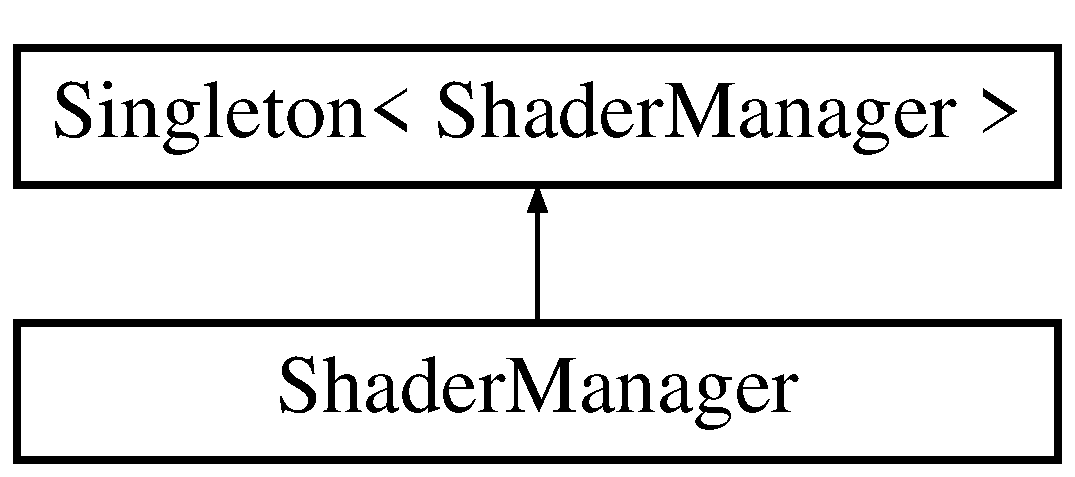
\includegraphics[height=2.000000cm]{class_d3_d11_1_1_graphic_1_1_shader_manager}
\end{center}
\end{figure}
\subsection*{公開メンバ関数}
\begin{DoxyCompactItemize}
\item 
\hyperlink{class_d3_d11_1_1_graphic_1_1_shader_manager_ade88b9cd89dfb4eb95b0cb874bf7168b}{$\sim$\+Shader\+Manager} ()\hypertarget{class_d3_d11_1_1_graphic_1_1_shader_manager_ade88b9cd89dfb4eb95b0cb874bf7168b}{}\label{class_d3_d11_1_1_graphic_1_1_shader_manager_ade88b9cd89dfb4eb95b0cb874bf7168b}

\begin{DoxyCompactList}\small\item\em デストラクタ \end{DoxyCompactList}\item 
H\+R\+E\+S\+U\+LT \hyperlink{class_d3_d11_1_1_graphic_1_1_shader_manager_ab30239875f87b8ad6c72cbc7eec479d4}{Add\+New\+Shader\+Data} (std\+::string sz\+Key\+Name, \hyperlink{struct_d3_d11_1_1_graphic_1_1_shader_data}{Shader\+Data} $\ast$p\+New\+Shader\+Data)
\item 
H\+R\+E\+S\+U\+LT \hyperlink{class_d3_d11_1_1_graphic_1_1_shader_manager_a206789dcc6ac911b3169d0dd706bfee6}{Initialize} (std\+::string directory\+Path=\char`\"{}\char`\"{})
\item 
void {\bfseries Finalize} ()\hypertarget{class_d3_d11_1_1_graphic_1_1_shader_manager_a8fee61d7a783cade1a3d07fe86284d27}{}\label{class_d3_d11_1_1_graphic_1_1_shader_manager_a8fee61d7a783cade1a3d07fe86284d27}

\item 
H\+R\+E\+S\+U\+LT \hyperlink{class_d3_d11_1_1_graphic_1_1_shader_manager_a5b52aad68e2e1517b8d6e74905d5d2f2}{Make\+Shader} (std\+::string sz\+File\+Name, std\+::string sz\+Func\+Name, std\+::string sz\+Profile\+Name, void $\ast$$\ast$pp\+Shader, I\+D3\+D\+Blob $\ast$$\ast$pp\+Blob)
\item 
\hyperlink{struct_d3_d11_1_1_graphic_1_1_shader_data}{Shader\+Data} $\ast$ \hyperlink{class_d3_d11_1_1_graphic_1_1_shader_manager_af58328bedb1bcde75d4beed5cdb431c1}{Get\+Shader\+Data} (std\+::string sz\+Key\+Name)\hypertarget{class_d3_d11_1_1_graphic_1_1_shader_manager_af58328bedb1bcde75d4beed5cdb431c1}{}\label{class_d3_d11_1_1_graphic_1_1_shader_manager_af58328bedb1bcde75d4beed5cdb431c1}

\begin{DoxyCompactList}\small\item\em キー(文字列)から登録済みのシェーダー情報を取得する  探索文字列から情報を取得することに失敗した場合\+N\+U\+L\+Lを返す \end{DoxyCompactList}\end{DoxyCompactItemize}
\subsection*{静的公開変数類}
\begin{DoxyCompactItemize}
\item 
static const std\+::string \hyperlink{class_d3_d11_1_1_graphic_1_1_shader_manager_a40c965cdd249ce2492b6f554987c9c71}{c\+\_\+sz\+Simple\+Texture\+Shader} = \char`\"{}S\+I\+M\+P\+L\+E\+\_\+\+T\+E\+X\+T\+U\+RE\char`\"{}
\begin{DoxyCompactList}\small\item\em 通常テクスチャで使うシェーダーのハッシュ  unordered\+\_\+mapに追加したシェーダーデータの参照用のハッシュ \end{DoxyCompactList}\item 
static const std\+::string \hyperlink{class_d3_d11_1_1_graphic_1_1_shader_manager_af418a1f0ddd33cf8dd7765f88c05aa3b}{c\+\_\+sz\+Texture\+Atlas\+Shader} = \char`\"{}A\+T\+L\+A\+S\+\_\+\+T\+E\+X\+T\+U\+RE\char`\"{}
\begin{DoxyCompactList}\small\item\em アトラステクスチャで使うシェーダーのハッシュ  unordered\+\_\+mapに追加したシェーダーデータの参照用のハッシュ \end{DoxyCompactList}\item 
static const std\+::string \hyperlink{class_d3_d11_1_1_graphic_1_1_shader_manager_ad1607cbc05176bb70e3699dd651b4674}{c\+\_\+\+Default\+Mesh\+Shader} = \char`\"{}M\+E\+S\+H\+\_\+\+D\+E\+F\+A\+U\+LT\char`\"{}
\begin{DoxyCompactList}\small\item\em デフォルト設定のメッシュで使うシェーダーのハッシュ  unordered\+\_\+mapに追加したシェーダーデータの参照用のハッシュ \end{DoxyCompactList}\end{DoxyCompactItemize}
\subsection*{非公開メンバ関数}
\begin{DoxyCompactItemize}
\item 
\hyperlink{class_d3_d11_1_1_graphic_1_1_shader_manager_a2dbca1784769d0a8bdfdd0c86a85464b}{Shader\+Manager} ()\hypertarget{class_d3_d11_1_1_graphic_1_1_shader_manager_a2dbca1784769d0a8bdfdd0c86a85464b}{}\label{class_d3_d11_1_1_graphic_1_1_shader_manager_a2dbca1784769d0a8bdfdd0c86a85464b}

\begin{DoxyCompactList}\small\item\em コンストラクタ \end{DoxyCompactList}\end{DoxyCompactItemize}
\subsection*{非公開変数類}
\begin{DoxyCompactItemize}
\item 
std\+::string \hyperlink{class_d3_d11_1_1_graphic_1_1_shader_manager_a6db27edfd24d67c38ce9d0d3d3903c97}{m\+\_\+\+Directory\+Path}\hypertarget{class_d3_d11_1_1_graphic_1_1_shader_manager_a6db27edfd24d67c38ce9d0d3d3903c97}{}\label{class_d3_d11_1_1_graphic_1_1_shader_manager_a6db27edfd24d67c38ce9d0d3d3903c97}

\begin{DoxyCompactList}\small\item\em シェーダー(.hlsl)が含まれているディレクトリのパス  Make\+Shaderはこのパス+ファイルの名前のパスに存在する\+H\+L\+S\+Lファイルでシェーダーの作成を行う \end{DoxyCompactList}\item 
\hyperlink{struct_d3_d11_1_1_graphic_1_1_shader_data}{Shader\+Data} $\ast$ \hyperlink{class_d3_d11_1_1_graphic_1_1_shader_manager_a0ea8d31a9751d1cae5e578665a53868f}{m\+\_\+p\+Add\+Data\+Ref}\hypertarget{class_d3_d11_1_1_graphic_1_1_shader_manager_a0ea8d31a9751d1cae5e578665a53868f}{}\label{class_d3_d11_1_1_graphic_1_1_shader_manager_a0ea8d31a9751d1cae5e578665a53868f}

\begin{DoxyCompactList}\small\item\em データ追加用の参照メンバ \end{DoxyCompactList}\item 
std\+::unordered\+\_\+map$<$ std\+::string, \hyperlink{struct_d3_d11_1_1_graphic_1_1_shader_data}{Shader\+Data} $\ast$ $>$ \hyperlink{class_d3_d11_1_1_graphic_1_1_shader_manager_a4fe3ad1dce5bc1d7d5169ebb4e6bb975}{m\+\_\+p\+Shader\+Data\+U\+Map}\hypertarget{class_d3_d11_1_1_graphic_1_1_shader_manager_a4fe3ad1dce5bc1d7d5169ebb4e6bb975}{}\label{class_d3_d11_1_1_graphic_1_1_shader_manager_a4fe3ad1dce5bc1d7d5169ebb4e6bb975}

\begin{DoxyCompactList}\small\item\em シェーダーデータの連想配列 \end{DoxyCompactList}\end{DoxyCompactItemize}
\subsection*{フレンド}
\begin{DoxyCompactItemize}
\item 
class \hyperlink{class_d3_d11_1_1_graphic_1_1_shader_manager_af5133f3fc6a5b6505ff2999082634c07}{Singleton$<$ Shader\+Manager $>$}\hypertarget{class_d3_d11_1_1_graphic_1_1_shader_manager_af5133f3fc6a5b6505ff2999082634c07}{}\label{class_d3_d11_1_1_graphic_1_1_shader_manager_af5133f3fc6a5b6505ff2999082634c07}

\begin{DoxyCompactList}\small\item\em シングルトンデザインパターンのテンプレート継承 \end{DoxyCompactList}\end{DoxyCompactItemize}
\subsection*{その他の継承メンバ}


\subsection{詳解}
シェーダー管理クラス  シェーダーを作成せずとも描画出来るデフォルトシェーダーを用意する 

\subsection{関数詳解}
\index{D3\+D11\+::\+Graphic\+::\+Shader\+Manager@{D3\+D11\+::\+Graphic\+::\+Shader\+Manager}!Add\+New\+Shader\+Data@{Add\+New\+Shader\+Data}}
\index{Add\+New\+Shader\+Data@{Add\+New\+Shader\+Data}!D3\+D11\+::\+Graphic\+::\+Shader\+Manager@{D3\+D11\+::\+Graphic\+::\+Shader\+Manager}}
\subsubsection[{\texorpdfstring{Add\+New\+Shader\+Data(std\+::string sz\+Key\+Name, Shader\+Data $\ast$p\+New\+Shader\+Data)}{AddNewShaderData(std::string szKeyName, ShaderData *pNewShaderData)}}]{\setlength{\rightskip}{0pt plus 5cm}H\+R\+E\+S\+U\+LT Add\+New\+Shader\+Data (
\begin{DoxyParamCaption}
\item[{std\+::string}]{sz\+Key\+Name, }
\item[{{\bf Shader\+Data} $\ast$}]{p\+New\+Shader\+Data}
\end{DoxyParamCaption}
)}\hypertarget{class_d3_d11_1_1_graphic_1_1_shader_manager_ab30239875f87b8ad6c72cbc7eec479d4}{}\label{class_d3_d11_1_1_graphic_1_1_shader_manager_ab30239875f87b8ad6c72cbc7eec479d4}
登録可能か判定

登録しようとしたキー名は既に登録済みのため追加しない

キー名でリスト(map)に追加 \index{D3\+D11\+::\+Graphic\+::\+Shader\+Manager@{D3\+D11\+::\+Graphic\+::\+Shader\+Manager}!Initialize@{Initialize}}
\index{Initialize@{Initialize}!D3\+D11\+::\+Graphic\+::\+Shader\+Manager@{D3\+D11\+::\+Graphic\+::\+Shader\+Manager}}
\subsubsection[{\texorpdfstring{Initialize(std\+::string directory\+Path="""")}{Initialize(std::string directoryPath="")}}]{\setlength{\rightskip}{0pt plus 5cm}H\+R\+E\+S\+U\+LT Initialize (
\begin{DoxyParamCaption}
\item[{std\+::string}]{directory\+Path = {\ttfamily \char`\"{}\char`\"{}}}
\end{DoxyParamCaption}
)}\hypertarget{class_d3_d11_1_1_graphic_1_1_shader_manager_a206789dcc6ac911b3169d0dd706bfee6}{}\label{class_d3_d11_1_1_graphic_1_1_shader_manager_a206789dcc6ac911b3169d0dd706bfee6}
$<$ コンパイル用ブロブ

リソースデイレクトリーの設定

単純テクスチャのシェーダー設定作成

バーテックスシェーダーの作成

頂点インプットレイアウト定義

$<$ ポインタ

頂点インプットレイアウトを作成

ピクセルシェーダーの作成

コンスタントバッファ定義

コンスタントバッファ作成

アトラステクスチャのシェーダー設定作成

・インプットレイアウト ・頂点シェーダー ・ピクセルシェーダー この三つは単純なテクスチャの\+Shaderと同じものを使う

インプットレイアウト

頂点シェーダー

ピクセルシェーダー

コンスタントバッファ定義

コンスタントバッファ作成

ブロブの解放

メッシュ用のデフォルト設定 \index{D3\+D11\+::\+Graphic\+::\+Shader\+Manager@{D3\+D11\+::\+Graphic\+::\+Shader\+Manager}!Make\+Shader@{Make\+Shader}}
\index{Make\+Shader@{Make\+Shader}!D3\+D11\+::\+Graphic\+::\+Shader\+Manager@{D3\+D11\+::\+Graphic\+::\+Shader\+Manager}}
\subsubsection[{\texorpdfstring{Make\+Shader(std\+::string sz\+File\+Name, std\+::string sz\+Func\+Name, std\+::string sz\+Profile\+Name, void $\ast$$\ast$pp\+Shader, I\+D3\+D\+Blob $\ast$$\ast$pp\+Blob)}{MakeShader(std::string szFileName, std::string szFuncName, std::string szProfileName, void **ppShader, ID3DBlob **ppBlob)}}]{\setlength{\rightskip}{0pt plus 5cm}H\+R\+E\+S\+U\+LT Make\+Shader (
\begin{DoxyParamCaption}
\item[{std\+::string}]{sz\+File\+Name, }
\item[{std\+::string}]{sz\+Func\+Name, }
\item[{std\+::string}]{sz\+Profile\+Name, }
\item[{void $\ast$$\ast$}]{pp\+Shader, }
\item[{I\+D3\+D\+Blob $\ast$$\ast$}]{pp\+Blob}
\end{DoxyParamCaption}
)}\hypertarget{class_d3_d11_1_1_graphic_1_1_shader_manager_a5b52aad68e2e1517b8d6e74905d5d2f2}{}\label{class_d3_d11_1_1_graphic_1_1_shader_manager_a5b52aad68e2e1517b8d6e74905d5d2f2}
U\+N\+I\+C\+O\+D\+E、マルチバイト両対応用文字列変換

D3\+D11\+Compile\+From\+Fileの引数はマルチバイト

ブロブのコンパイル

終端文字を含まないバッファのメモリを変数にコピー

$<$ 終端文字のバッファーを一つ確保しておく

頂点シェーダー(\+Vertex Shader)

ピクセルシェーダー(\+Pixel Shader)

ジオメトリシェーダー(\+Geometry Shader)

ハルシェーダー(\+Hull Shader)

ドメインシェーダー(\+Domain Shader)

コンピュートシェーダー(\+Compute Shader) 

\subsection{メンバ詳解}
\index{D3\+D11\+::\+Graphic\+::\+Shader\+Manager@{D3\+D11\+::\+Graphic\+::\+Shader\+Manager}!c\+\_\+\+Default\+Mesh\+Shader@{c\+\_\+\+Default\+Mesh\+Shader}}
\index{c\+\_\+\+Default\+Mesh\+Shader@{c\+\_\+\+Default\+Mesh\+Shader}!D3\+D11\+::\+Graphic\+::\+Shader\+Manager@{D3\+D11\+::\+Graphic\+::\+Shader\+Manager}}
\subsubsection[{\texorpdfstring{c\+\_\+\+Default\+Mesh\+Shader}{c_DefaultMeshShader}}]{\setlength{\rightskip}{0pt plus 5cm}c\+\_\+\+Default\+Mesh\+Shader = \char`\"{}M\+E\+S\+H\+\_\+\+D\+E\+F\+A\+U\+LT\char`\"{}\hspace{0.3cm}{\ttfamily [static]}}\hypertarget{class_d3_d11_1_1_graphic_1_1_shader_manager_ad1607cbc05176bb70e3699dd651b4674}{}\label{class_d3_d11_1_1_graphic_1_1_shader_manager_ad1607cbc05176bb70e3699dd651b4674}


デフォルト設定のメッシュで使うシェーダーのハッシュ  unordered\+\_\+mapに追加したシェーダーデータの参照用のハッシュ 

メッシュシェーダーのデフォルト設定 \index{D3\+D11\+::\+Graphic\+::\+Shader\+Manager@{D3\+D11\+::\+Graphic\+::\+Shader\+Manager}!c\+\_\+sz\+Simple\+Texture\+Shader@{c\+\_\+sz\+Simple\+Texture\+Shader}}
\index{c\+\_\+sz\+Simple\+Texture\+Shader@{c\+\_\+sz\+Simple\+Texture\+Shader}!D3\+D11\+::\+Graphic\+::\+Shader\+Manager@{D3\+D11\+::\+Graphic\+::\+Shader\+Manager}}
\subsubsection[{\texorpdfstring{c\+\_\+sz\+Simple\+Texture\+Shader}{c_szSimpleTextureShader}}]{\setlength{\rightskip}{0pt plus 5cm}c\+\_\+sz\+Simple\+Texture\+Shader = \char`\"{}S\+I\+M\+P\+L\+E\+\_\+\+T\+E\+X\+T\+U\+RE\char`\"{}\hspace{0.3cm}{\ttfamily [static]}}\hypertarget{class_d3_d11_1_1_graphic_1_1_shader_manager_a40c965cdd249ce2492b6f554987c9c71}{}\label{class_d3_d11_1_1_graphic_1_1_shader_manager_a40c965cdd249ce2492b6f554987c9c71}


通常テクスチャで使うシェーダーのハッシュ  unordered\+\_\+mapに追加したシェーダーデータの参照用のハッシュ 

シンプルテクスチャのシェーダー \index{D3\+D11\+::\+Graphic\+::\+Shader\+Manager@{D3\+D11\+::\+Graphic\+::\+Shader\+Manager}!c\+\_\+sz\+Texture\+Atlas\+Shader@{c\+\_\+sz\+Texture\+Atlas\+Shader}}
\index{c\+\_\+sz\+Texture\+Atlas\+Shader@{c\+\_\+sz\+Texture\+Atlas\+Shader}!D3\+D11\+::\+Graphic\+::\+Shader\+Manager@{D3\+D11\+::\+Graphic\+::\+Shader\+Manager}}
\subsubsection[{\texorpdfstring{c\+\_\+sz\+Texture\+Atlas\+Shader}{c_szTextureAtlasShader}}]{\setlength{\rightskip}{0pt plus 5cm}c\+\_\+sz\+Texture\+Atlas\+Shader = \char`\"{}A\+T\+L\+A\+S\+\_\+\+T\+E\+X\+T\+U\+RE\char`\"{}\hspace{0.3cm}{\ttfamily [static]}}\hypertarget{class_d3_d11_1_1_graphic_1_1_shader_manager_af418a1f0ddd33cf8dd7765f88c05aa3b}{}\label{class_d3_d11_1_1_graphic_1_1_shader_manager_af418a1f0ddd33cf8dd7765f88c05aa3b}


アトラステクスチャで使うシェーダーのハッシュ  unordered\+\_\+mapに追加したシェーダーデータの参照用のハッシュ 

アトラステクスチャのシェーダー 

このクラス詳解は次のファイルから抽出されました\+:\begin{DoxyCompactItemize}
\item 
C\+:/\+Users/yuuki/\+Desktop/\+Doxygen\+\_\+lib\+\_\+source/include/Shader\+Manager.\+h\item 
C\+:/\+Users/yuuki/\+Desktop/\+Doxygen\+\_\+lib\+\_\+source/include/Shader\+Manager.\+cpp\end{DoxyCompactItemize}

\hypertarget{class_singleton}{}\section{Singleton$<$ T $>$ クラステンプレート}
\label{class_singleton}\index{Singleton$<$ T $>$@{Singleton$<$ T $>$}}
\subsection*{静的公開メンバ関数}
\begin{DoxyCompactItemize}
\item 
static T \& \hyperlink{class_singleton_a0866aab4257483326c469dcef942f0e1}{Get\+Instance} ()
\end{DoxyCompactItemize}
\subsection*{限定公開メンバ関数}
\begin{DoxyCompactItemize}
\item 
\hyperlink{class_singleton_a04783ca27b0280a844368faf849c8ddb}{Singleton} ()
\item 
virtual \hyperlink{class_singleton_a7d833a82cba7b9c4083d4c071a771cfc}{$\sim$\+Singleton} ()
\end{DoxyCompactItemize}
\subsection*{非公開メンバ関数}
\begin{DoxyCompactItemize}
\item 
void \hyperlink{class_singleton_a1915f268d5672b8a0650412218f39110}{operator=} (const \hyperlink{class_singleton}{Singleton} \&)=delete
\item 
\hyperlink{class_singleton_a4261e9a2454202cd68bdb9c2fa4bf294}{Singleton} (const \hyperlink{class_singleton}{Singleton} \&)=delete
\end{DoxyCompactItemize}


\subsection{構築子と解体子}
\index{Singleton@{Singleton}!Singleton@{Singleton}}
\index{Singleton@{Singleton}!Singleton@{Singleton}}
\subsubsection[{\texorpdfstring{Singleton()}{Singleton()}}]{\setlength{\rightskip}{0pt plus 5cm}{\bf Singleton} (
\begin{DoxyParamCaption}
{}
\end{DoxyParamCaption}
)\hspace{0.3cm}{\ttfamily [inline]}, {\ttfamily [protected]}}\hypertarget{class_singleton_a04783ca27b0280a844368faf849c8ddb}{}\label{class_singleton_a04783ca27b0280a844368faf849c8ddb}
空コンストラクタ \index{Singleton@{Singleton}!````~Singleton@{$\sim$\+Singleton}}
\index{````~Singleton@{$\sim$\+Singleton}!Singleton@{Singleton}}
\subsubsection[{\texorpdfstring{$\sim$\+Singleton()}{~Singleton()}}]{\setlength{\rightskip}{0pt plus 5cm}virtual $\sim${\bf Singleton} (
\begin{DoxyParamCaption}
{}
\end{DoxyParamCaption}
)\hspace{0.3cm}{\ttfamily [inline]}, {\ttfamily [protected]}, {\ttfamily [virtual]}}\hypertarget{class_singleton_a7d833a82cba7b9c4083d4c071a771cfc}{}\label{class_singleton_a7d833a82cba7b9c4083d4c071a771cfc}
仮想デストラクタ \index{Singleton@{Singleton}!Singleton@{Singleton}}
\index{Singleton@{Singleton}!Singleton@{Singleton}}
\subsubsection[{\texorpdfstring{Singleton(const Singleton \&)=delete}{Singleton(const Singleton &)=delete}}]{\setlength{\rightskip}{0pt plus 5cm}{\bf Singleton} (
\begin{DoxyParamCaption}
\item[{const {\bf Singleton}$<$ T $>$ \&}]{}
\end{DoxyParamCaption}
)\hspace{0.3cm}{\ttfamily [private]}, {\ttfamily [delete]}}\hypertarget{class_singleton_a4261e9a2454202cd68bdb9c2fa4bf294}{}\label{class_singleton_a4261e9a2454202cd68bdb9c2fa4bf294}
コピーコンストラクタ削除 

\subsection{関数詳解}
\index{Singleton@{Singleton}!Get\+Instance@{Get\+Instance}}
\index{Get\+Instance@{Get\+Instance}!Singleton@{Singleton}}
\subsubsection[{\texorpdfstring{Get\+Instance()}{GetInstance()}}]{\setlength{\rightskip}{0pt plus 5cm}static T\& Get\+Instance (
\begin{DoxyParamCaption}
{}
\end{DoxyParamCaption}
)\hspace{0.3cm}{\ttfamily [inline]}, {\ttfamily [static]}}\hypertarget{class_singleton_a0866aab4257483326c469dcef942f0e1}{}\label{class_singleton_a0866aab4257483326c469dcef942f0e1}
インスタンスのゲッター \index{Singleton@{Singleton}!operator=@{operator=}}
\index{operator=@{operator=}!Singleton@{Singleton}}
\subsubsection[{\texorpdfstring{operator=(const Singleton \&)=delete}{operator=(const Singleton &)=delete}}]{\setlength{\rightskip}{0pt plus 5cm}void operator= (
\begin{DoxyParamCaption}
\item[{const {\bf Singleton}$<$ T $>$ \&}]{}
\end{DoxyParamCaption}
)\hspace{0.3cm}{\ttfamily [private]}, {\ttfamily [delete]}}\hypertarget{class_singleton_a1915f268d5672b8a0650412218f39110}{}\label{class_singleton_a1915f268d5672b8a0650412218f39110}
代入オペレーター削除 

このクラス詳解は次のファイルから抽出されました\+:\begin{DoxyCompactItemize}
\item 
C\+:/\+Users/yuuki/\+Desktop/\+Doxygen\+\_\+lib\+\_\+source/include/Singleton.\+h\end{DoxyCompactItemize}

\hypertarget{class_a_p_i_1_1_sprite}{}\section{Sprite クラス}
\label{class_a_p_i_1_1_sprite}\index{Sprite@{Sprite}}


{\ttfamily \#include $<$Sprite.\+h$>$}

\subsection*{公開メンバ関数}
\begin{DoxyCompactItemize}
\item 
\hyperlink{class_a_p_i_1_1_sprite_a637dbaba7024234f1dd304df1706c371}{Sprite} ()\hypertarget{class_a_p_i_1_1_sprite_a637dbaba7024234f1dd304df1706c371}{}\label{class_a_p_i_1_1_sprite_a637dbaba7024234f1dd304df1706c371}

\begin{DoxyCompactList}\small\item\em コンストラクタ \end{DoxyCompactList}\item 
\hyperlink{class_a_p_i_1_1_sprite_ae2ec7be3ca7853c7f3ac5d639b6b951d}{$\sim$\+Sprite} ()\hypertarget{class_a_p_i_1_1_sprite_ae2ec7be3ca7853c7f3ac5d639b6b951d}{}\label{class_a_p_i_1_1_sprite_ae2ec7be3ca7853c7f3ac5d639b6b951d}

\begin{DoxyCompactList}\small\item\em デストラクタ \end{DoxyCompactList}\item 
H\+R\+E\+S\+U\+LT \hyperlink{class_a_p_i_1_1_sprite_a81109341187e54cc3585f29a1306ca50}{Initialize} ()
\item 
void \hyperlink{class_a_p_i_1_1_sprite_a8fee61d7a783cade1a3d07fe86284d27}{Finalize} ()
\item 
void {\bfseries Release} ()\hypertarget{class_a_p_i_1_1_sprite_a94c93747c8daa99d65c2a04c6be0748c}{}\label{class_a_p_i_1_1_sprite_a94c93747c8daa99d65c2a04c6be0748c}

\item 
H\+R\+E\+S\+U\+LT \hyperlink{class_a_p_i_1_1_sprite_af9c6b795e8d45972269d3fdc8cf9a3c4}{Render} (\hyperlink{class_a_p_i_1_1_texture}{Texture} $\ast$p\+Texture)
\item 
H\+R\+E\+S\+U\+LT \hyperlink{class_a_p_i_1_1_sprite_abea1a725dece7f8198dd4f0f9e95afb8}{Render} (\hyperlink{class_a_p_i_1_1_texture_atlas}{Texture\+Atlas} $\ast$p\+Texture)
\item 
H\+R\+E\+S\+U\+LT \hyperlink{class_a_p_i_1_1_sprite_a0d7e8aacecb8e343ea166b614398ce12}{Render\+Tile} (\hyperlink{class_a_p_i_1_1_texture}{Texture} $\ast$p\+Texture, const Direct\+X\+::\+X\+M\+F\+L\+O\+A\+T2 ratio)
\item 
Direct\+X\+::\+X\+M\+F\+L\+O\+A\+T3 \hyperlink{class_a_p_i_1_1_sprite_a471a0be5d782804468865b18a3eca5f1}{Get\+Pos} () const 
\item 
void \hyperlink{class_a_p_i_1_1_sprite_a966d3c6ff7e6bee56d3d8576d4585037}{Set\+Pos} (Direct\+X\+::\+X\+M\+F\+L\+O\+A\+T3 pos)\hypertarget{class_a_p_i_1_1_sprite_a966d3c6ff7e6bee56d3d8576d4585037}{}\label{class_a_p_i_1_1_sprite_a966d3c6ff7e6bee56d3d8576d4585037}

\begin{DoxyCompactList}\small\item\em 座標のセッター \end{DoxyCompactList}\item 
void \hyperlink{class_a_p_i_1_1_sprite_a40cf3dffabd00db79c9a7a70ade8ad16}{Set\+Pos} (Direct\+X\+::\+X\+M\+F\+L\+O\+A\+T2 pos)\hypertarget{class_a_p_i_1_1_sprite_a40cf3dffabd00db79c9a7a70ade8ad16}{}\label{class_a_p_i_1_1_sprite_a40cf3dffabd00db79c9a7a70ade8ad16}

\begin{DoxyCompactList}\small\item\em 座標のセッター  オーバーロード \end{DoxyCompactList}\item 
void {\bfseries Set\+Rot} (Direct\+X\+::\+X\+M\+F\+L\+O\+A\+T3 rot)\hypertarget{class_a_p_i_1_1_sprite_ac99b0e85c8f96e81093cbc13036aa07b}{}\label{class_a_p_i_1_1_sprite_ac99b0e85c8f96e81093cbc13036aa07b}

\item 
void \hyperlink{class_a_p_i_1_1_sprite_a4800713a43bf7b867abef7ad679ceb85}{Set\+Scale} (Direct\+X\+::\+X\+M\+F\+L\+O\+A\+T2 scale)\hypertarget{class_a_p_i_1_1_sprite_a4800713a43bf7b867abef7ad679ceb85}{}\label{class_a_p_i_1_1_sprite_a4800713a43bf7b867abef7ad679ceb85}

\begin{DoxyCompactList}\small\item\em スケールのセッター \end{DoxyCompactList}\item 
void {\bfseries Set\+Stencil\+Mask} (uint32\+\_\+t mask)\hypertarget{class_a_p_i_1_1_sprite_a016dc5cfc0bd53f3653b1ba35b4e6a17}{}\label{class_a_p_i_1_1_sprite_a016dc5cfc0bd53f3653b1ba35b4e6a17}

\item 
void \hyperlink{class_a_p_i_1_1_sprite_a043d0d75b247c2db2f011dc8b8621e58}{Create\+Alpha\+Blend\+State} (D3\+D11\+\_\+\+B\+L\+E\+N\+D\+\_\+\+D\+E\+SC desc)
\end{DoxyCompactItemize}
\subsection*{非公開メンバ関数}
\begin{DoxyCompactItemize}
\item 
H\+R\+E\+S\+U\+LT \hyperlink{class_a_p_i_1_1_sprite_a8629113e859e0772382f67b6de6036bc}{Create\+Vertex} (Direct\+X\+::\+X\+M\+I\+N\+T2 size)
\item 
H\+R\+E\+S\+U\+LT \hyperlink{class_a_p_i_1_1_sprite_acc51e83897641c917cf8e2883519bd7c}{Create\+Tiling\+Vertex} (Direct\+X\+::\+X\+M\+I\+N\+T2 size, Direct\+X\+::\+X\+M\+F\+L\+O\+A\+T2 ratio)
\end{DoxyCompactItemize}
\subsection*{非公開変数類}
\begin{DoxyCompactItemize}
\item 
uint32\+\_\+t {\bfseries m\+\_\+\+Stencil\+Mask}\hypertarget{class_a_p_i_1_1_sprite_a14c9f660773821f8d9005b415e1b9c78}{}\label{class_a_p_i_1_1_sprite_a14c9f660773821f8d9005b415e1b9c78}

\item 
Microsoft\+::\+W\+R\+L\+::\+Com\+Ptr$<$ I\+D3\+D11\+Buffer $>$ {\bfseries m\+\_\+p\+Vertex\+Buffer}\hypertarget{class_a_p_i_1_1_sprite_aefe7709234a1ba240773c9794032a88c}{}\label{class_a_p_i_1_1_sprite_aefe7709234a1ba240773c9794032a88c}

\item 
Microsoft\+::\+W\+R\+L\+::\+Com\+Ptr$<$ I\+D3\+D11\+Blend\+State $>$ {\bfseries m\+\_\+p\+Blend\+State}\hypertarget{class_a_p_i_1_1_sprite_a63001d1ec2d9ac02687c99306af4a07f}{}\label{class_a_p_i_1_1_sprite_a63001d1ec2d9ac02687c99306af4a07f}

\item 
Microsoft\+::\+W\+R\+L\+::\+Com\+Ptr$<$ I\+D3\+D11\+Blend\+State $>$ {\bfseries m\+\_\+p\+Blend\+State\+Multiple}\hypertarget{class_a_p_i_1_1_sprite_a05d37dc5f363ce48454bc3bd9b508d9f}{}\label{class_a_p_i_1_1_sprite_a05d37dc5f363ce48454bc3bd9b508d9f}

\item 
Direct\+X\+::\+X\+M\+F\+L\+O\+A\+T3 \hyperlink{class_a_p_i_1_1_sprite_ac4dfe78085ef0a056c1ec0b18bbf894b}{m\+\_\+\+Pos}
\item 
Direct\+X\+::\+X\+M\+F\+L\+O\+A\+T3 {\bfseries m\+\_\+\+Rot}\hypertarget{class_a_p_i_1_1_sprite_a90e58aea364e265ec25080e06f3e6c3f}{}\label{class_a_p_i_1_1_sprite_a90e58aea364e265ec25080e06f3e6c3f}

\item 
Direct\+X\+::\+X\+M\+F\+L\+O\+A\+T3 {\bfseries m\+\_\+\+Scale}\hypertarget{class_a_p_i_1_1_sprite_ad778260919c8cf3a968b962f588ca7a5}{}\label{class_a_p_i_1_1_sprite_ad778260919c8cf3a968b962f588ca7a5}

\item 
Direct\+X\+::\+X\+M\+I\+N\+T2 \hyperlink{class_a_p_i_1_1_sprite_adb6dc678fde02000203c71a186713543}{m\+\_\+\+Size}
\end{DoxyCompactItemize}
\subsection*{静的非公開変数類}
\begin{DoxyCompactItemize}
\item 
static constexpr int \hyperlink{class_a_p_i_1_1_sprite_a7d0612770885bd905daaa74dee3eaca5}{c\+\_\+\+Vertex\+Count} = 4
\begin{DoxyCompactList}\small\item\em スプライトの頂点数  スプライトの頂点数の定数化 \end{DoxyCompactList}\item 
static const float \hyperlink{class_a_p_i_1_1_sprite_ad77d7d33858bc5288514fc4bad99a983}{c\+\_\+\+Normalize\+Size} = 100.\+0f
\begin{DoxyCompactList}\small\item\em 基準となるサイズ  このピクセルが\+Scaleの1に相当する  100.\+0f \end{DoxyCompactList}\item 
static const float \hyperlink{class_a_p_i_1_1_sprite_ad804c9e981cc840e5629fd162893744b}{c\+\_\+\+ScaleZ} = 0
\begin{DoxyCompactList}\small\item\em 板ポリの\+Zスケール  生成する頂点の\+Z方向の大きさ  0 \end{DoxyCompactList}\item 
static const float \hyperlink{class_a_p_i_1_1_sprite_a9c8bd1ba9b75570d1ad44479a342fedc}{c\+\_\+\+VertexZ} = 0
\begin{DoxyCompactList}\small\item\em 板ポリの頂点生成位置  Create\+Vertex関数で生成する頂点の\+Z位置  0 \end{DoxyCompactList}\end{DoxyCompactItemize}


\subsection{詳解}
スプライトを扱うクラス 

\subsection{関数詳解}
\index{A\+P\+I\+::\+Sprite@{A\+P\+I\+::\+Sprite}!Create\+Alpha\+Blend\+State@{Create\+Alpha\+Blend\+State}}
\index{Create\+Alpha\+Blend\+State@{Create\+Alpha\+Blend\+State}!A\+P\+I\+::\+Sprite@{A\+P\+I\+::\+Sprite}}
\subsubsection[{\texorpdfstring{Create\+Alpha\+Blend\+State(\+D3\+D11\+\_\+\+B\+L\+E\+N\+D\+\_\+\+D\+E\+S\+C desc)}{CreateAlphaBlendState(D3D11_BLEND_DESC desc)}}]{\setlength{\rightskip}{0pt plus 5cm}void Create\+Alpha\+Blend\+State (
\begin{DoxyParamCaption}
\item[{D3\+D11\+\_\+\+B\+L\+E\+N\+D\+\_\+\+D\+E\+SC}]{desc}
\end{DoxyParamCaption}
)}\hypertarget{class_a_p_i_1_1_sprite_a043d0d75b247c2db2f011dc8b8621e58}{}\label{class_a_p_i_1_1_sprite_a043d0d75b247c2db2f011dc8b8621e58}
メモリ開放

ブレンドステート作成 \index{A\+P\+I\+::\+Sprite@{A\+P\+I\+::\+Sprite}!Create\+Tiling\+Vertex@{Create\+Tiling\+Vertex}}
\index{Create\+Tiling\+Vertex@{Create\+Tiling\+Vertex}!A\+P\+I\+::\+Sprite@{A\+P\+I\+::\+Sprite}}
\subsubsection[{\texorpdfstring{Create\+Tiling\+Vertex(\+Direct\+X\+::\+X\+M\+I\+N\+T2 size, Direct\+X\+::\+X\+M\+F\+L\+O\+A\+T2 ratio)}{CreateTilingVertex(DirectX::XMINT2 size, DirectX::XMFLOAT2 ratio)}}]{\setlength{\rightskip}{0pt plus 5cm}H\+R\+E\+S\+U\+LT Create\+Tiling\+Vertex (
\begin{DoxyParamCaption}
\item[{Direct\+X\+::\+X\+M\+I\+N\+T2}]{size, }
\item[{Direct\+X\+::\+X\+M\+F\+L\+O\+A\+T2}]{ratio}
\end{DoxyParamCaption}
)\hspace{0.3cm}{\ttfamily [private]}}\hypertarget{class_a_p_i_1_1_sprite_acc51e83897641c917cf8e2883519bd7c}{}\label{class_a_p_i_1_1_sprite_acc51e83897641c917cf8e2883519bd7c}
頂点宣言

$<$ 頂点座標

$<$ U\+V座標

U\+V定義

各頂点定義

$<$ 左

$<$ 右

$<$ 上

$<$ 下

頂点構造体定義

右上

頂点

U\+V座標

右下

頂点

U\+V座標

左上

頂点

U\+V座標

左下

頂点

U\+V座標

板ポリゴン(四角形ポリゴン)のバッファを定義

$<$ G\+P\+Uから読み込みと書き込みを許可

$<$ バッファのサイズ

$<$ 頂点バッファとしてレンダリングパイプラインにバインド

サブリソースのデータを定義

$<$ 初期化データへのポインタ

頂点バッファの開放

頂点バッファ生成 \index{A\+P\+I\+::\+Sprite@{A\+P\+I\+::\+Sprite}!Create\+Vertex@{Create\+Vertex}}
\index{Create\+Vertex@{Create\+Vertex}!A\+P\+I\+::\+Sprite@{A\+P\+I\+::\+Sprite}}
\subsubsection[{\texorpdfstring{Create\+Vertex(\+Direct\+X\+::\+X\+M\+I\+N\+T2 size)}{CreateVertex(DirectX::XMINT2 size)}}]{\setlength{\rightskip}{0pt plus 5cm}H\+R\+E\+S\+U\+LT Create\+Vertex (
\begin{DoxyParamCaption}
\item[{Direct\+X\+::\+X\+M\+I\+N\+T2}]{size}
\end{DoxyParamCaption}
)\hspace{0.3cm}{\ttfamily [private]}}\hypertarget{class_a_p_i_1_1_sprite_a8629113e859e0772382f67b6de6036bc}{}\label{class_a_p_i_1_1_sprite_a8629113e859e0772382f67b6de6036bc}
頂点宣言

$<$ 頂点座標

$<$ U\+V座標

各頂点定義

$<$ 左

$<$ 右

$<$ 上

$<$ 下

U\+V定義

頂点構造体定義

右上

頂点

U\+V座標

右下

頂点

U\+V座標

左上

頂点

U\+V座標

左下

頂点

U\+V座標

板ポリゴン(四角形ポリゴン)のバッファを定義

$<$ G\+P\+Uから読み込みと書き込みを許可

$<$ バッファのサイズ

$<$ 頂点バッファとしてレンダリングパイプラインにバインド

サブリソースのデータを定義

$<$ 初期化データへのポインタ

頂点バッファの開放

頂点バッファ生成

頂点バッファセット \index{A\+P\+I\+::\+Sprite@{A\+P\+I\+::\+Sprite}!Finalize@{Finalize}}
\index{Finalize@{Finalize}!A\+P\+I\+::\+Sprite@{A\+P\+I\+::\+Sprite}}
\subsubsection[{\texorpdfstring{Finalize()}{Finalize()}}]{\setlength{\rightskip}{0pt plus 5cm}void Finalize (
\begin{DoxyParamCaption}
{}
\end{DoxyParamCaption}
)}\hypertarget{class_a_p_i_1_1_sprite_a8fee61d7a783cade1a3d07fe86284d27}{}\label{class_a_p_i_1_1_sprite_a8fee61d7a783cade1a3d07fe86284d27}
メンバの初期化

開放 \index{A\+P\+I\+::\+Sprite@{A\+P\+I\+::\+Sprite}!Get\+Pos@{Get\+Pos}}
\index{Get\+Pos@{Get\+Pos}!A\+P\+I\+::\+Sprite@{A\+P\+I\+::\+Sprite}}
\subsubsection[{\texorpdfstring{Get\+Pos() const }{GetPos() const }}]{\setlength{\rightskip}{0pt plus 5cm}Direct\+X\+::\+X\+M\+F\+L\+O\+A\+T3 Get\+Pos (
\begin{DoxyParamCaption}
{}
\end{DoxyParamCaption}
) const\hspace{0.3cm}{\ttfamily [inline]}}\hypertarget{class_a_p_i_1_1_sprite_a471a0be5d782804468865b18a3eca5f1}{}\label{class_a_p_i_1_1_sprite_a471a0be5d782804468865b18a3eca5f1}
Transformクラスに書き直す予定 \index{A\+P\+I\+::\+Sprite@{A\+P\+I\+::\+Sprite}!Initialize@{Initialize}}
\index{Initialize@{Initialize}!A\+P\+I\+::\+Sprite@{A\+P\+I\+::\+Sprite}}
\subsubsection[{\texorpdfstring{Initialize()}{Initialize()}}]{\setlength{\rightskip}{0pt plus 5cm}H\+R\+E\+S\+U\+LT Initialize (
\begin{DoxyParamCaption}
{}
\end{DoxyParamCaption}
)}\hypertarget{class_a_p_i_1_1_sprite_a81109341187e54cc3585f29a1306ca50}{}\label{class_a_p_i_1_1_sprite_a81109341187e54cc3585f29a1306ca50}
※ S\+RC\+:ソース(これから描画するピクセルの色) D\+E\+ST\+:ディストネーション(レンダリングターゲットに描画されているピクセルの色)

最終的な描画色は以下の「混合関数」によって決まる \begin{DoxyVerb}SRC × ブレンディング係数 + DEST × ブレンディング係数

SRCALPHA:    SRC のα値
INVSRCALPHA: 1 - SRC のα値
DESTALPHA:   DESTのα値
\end{DoxyVerb}


αブレンド

αテスト設定

$<$ ブレンドの有効・無効

ブレンディング係数の設定

ブレンドオプション

アンチエイリアス処理

ブレンドステートの作成

ブレンドステートの設定 \index{A\+P\+I\+::\+Sprite@{A\+P\+I\+::\+Sprite}!Render@{Render}}
\index{Render@{Render}!A\+P\+I\+::\+Sprite@{A\+P\+I\+::\+Sprite}}
\subsubsection[{\texorpdfstring{Render(\+Texture $\ast$p\+Texture)}{Render(Texture *pTexture)}}]{\setlength{\rightskip}{0pt plus 5cm}H\+R\+E\+S\+U\+LT Render (
\begin{DoxyParamCaption}
\item[{{\bf Texture} $\ast$}]{p\+Texture}
\end{DoxyParamCaption}
)}\hypertarget{class_a_p_i_1_1_sprite_af9c6b795e8d45972269d3fdc8cf9a3c4}{}\label{class_a_p_i_1_1_sprite_af9c6b795e8d45972269d3fdc8cf9a3c4}
異なるサイズのテクスチャが渡されたら頂点生成

頂点バッファ生成

テクスチャのサイズをキャッシュしておく

トポロジーセット

頂点インプットレイアウトセット

シェーダーの登録

コンスタントバッファの登録

サンプラー取得

S\+R\+V取得

テクスチャ

座標変換

ワールド変換

マッピング用変数宣言

シェーダー側に渡すコンスタントバッファ宣言

バッファへのアクセス許可(書き換え)

$<$ アクセス権を閉じて抜ける

コンスタントバッファにデータを送る

$<$ ワールド行列

メモリコピー

アクセス許可終了

頂点バッファセット

ブレンドステートの設定

描画

$<$ 頂点数(板ポリゴンなので頂点数は4つ) \index{A\+P\+I\+::\+Sprite@{A\+P\+I\+::\+Sprite}!Render@{Render}}
\index{Render@{Render}!A\+P\+I\+::\+Sprite@{A\+P\+I\+::\+Sprite}}
\subsubsection[{\texorpdfstring{Render(\+Texture\+Atlas $\ast$p\+Texture)}{Render(TextureAtlas *pTexture)}}]{\setlength{\rightskip}{0pt plus 5cm}H\+R\+E\+S\+U\+LT Render (
\begin{DoxyParamCaption}
\item[{{\bf Texture\+Atlas} $\ast$}]{p\+Texture}
\end{DoxyParamCaption}
)}\hypertarget{class_a_p_i_1_1_sprite_abea1a725dece7f8198dd4f0f9e95afb8}{}\label{class_a_p_i_1_1_sprite_abea1a725dece7f8198dd4f0f9e95afb8}
頂点バッファ生成

テクスチャのサイズをキャッシュしておく

トポロジーセット

頂点インプットレイアウトセット

シェーダーの登録

コンスタントバッファの登録

サンプラー取得

S\+R\+V取得

テクスチャ

座標変換

ワールド変換

シェーダー側に渡すコンスタントバッファ宣言

コンスタントバッファのデータ書き換え

$<$ ワールド行列

Update\+Sub\+Resource

ブレンドステートの設定

描画

$<$ 頂点数(板ポリゴンなので頂点数は4つ) \index{A\+P\+I\+::\+Sprite@{A\+P\+I\+::\+Sprite}!Render\+Tile@{Render\+Tile}}
\index{Render\+Tile@{Render\+Tile}!A\+P\+I\+::\+Sprite@{A\+P\+I\+::\+Sprite}}
\subsubsection[{\texorpdfstring{Render\+Tile(\+Texture $\ast$p\+Texture, const Direct\+X\+::\+X\+M\+F\+L\+O\+A\+T2 ratio)}{RenderTile(Texture *pTexture, const DirectX::XMFLOAT2 ratio)}}]{\setlength{\rightskip}{0pt plus 5cm}H\+R\+E\+S\+U\+LT Render\+Tile (
\begin{DoxyParamCaption}
\item[{{\bf Texture} $\ast$}]{p\+Texture, }
\item[{const Direct\+X\+::\+X\+M\+F\+L\+O\+A\+T2}]{ratio}
\end{DoxyParamCaption}
)}\hypertarget{class_a_p_i_1_1_sprite_a0d7e8aacecb8e343ea166b614398ce12}{}\label{class_a_p_i_1_1_sprite_a0d7e8aacecb8e343ea166b614398ce12}
頂点生成

テクスチャのサイズをキャッシュしておく

トポロジーセット

頂点インプットレイアウトセット

シェーダーの登録

コンスタントバッファの登録

サンプラー取得

S\+R\+V取得

テクスチャ

座標変換

ワールド変換

シェーダー側に渡すコンスタントバッファ宣言

コンスタントバッファのデータ書き換え

$<$ ワールド行列

Update\+Sub\+Resource

頂点バッファセット

ブレンドステートの設定

描画

$<$ 頂点数(板ポリゴンなので頂点数は4つ) 

\subsection{メンバ詳解}
\index{A\+P\+I\+::\+Sprite@{A\+P\+I\+::\+Sprite}!c\+\_\+\+Normalize\+Size@{c\+\_\+\+Normalize\+Size}}
\index{c\+\_\+\+Normalize\+Size@{c\+\_\+\+Normalize\+Size}!A\+P\+I\+::\+Sprite@{A\+P\+I\+::\+Sprite}}
\subsubsection[{\texorpdfstring{c\+\_\+\+Normalize\+Size}{c_NormalizeSize}}]{\setlength{\rightskip}{0pt plus 5cm}c\+\_\+\+Normalize\+Size = 100.\+0f\hspace{0.3cm}{\ttfamily [static]}, {\ttfamily [private]}}\hypertarget{class_a_p_i_1_1_sprite_ad77d7d33858bc5288514fc4bad99a983}{}\label{class_a_p_i_1_1_sprite_ad77d7d33858bc5288514fc4bad99a983}


基準となるサイズ  このピクセルが\+Scaleの1に相当する  100.\+0f 

スケールが1の時の基準となるサイズ(100×100が大きさの基準) \index{A\+P\+I\+::\+Sprite@{A\+P\+I\+::\+Sprite}!c\+\_\+\+ScaleZ@{c\+\_\+\+ScaleZ}}
\index{c\+\_\+\+ScaleZ@{c\+\_\+\+ScaleZ}!A\+P\+I\+::\+Sprite@{A\+P\+I\+::\+Sprite}}
\subsubsection[{\texorpdfstring{c\+\_\+\+ScaleZ}{c_ScaleZ}}]{\setlength{\rightskip}{0pt plus 5cm}c\+\_\+\+ScaleZ = 0\hspace{0.3cm}{\ttfamily [static]}, {\ttfamily [private]}}\hypertarget{class_a_p_i_1_1_sprite_ad804c9e981cc840e5629fd162893744b}{}\label{class_a_p_i_1_1_sprite_ad804c9e981cc840e5629fd162893744b}


板ポリの\+Zスケール  生成する頂点の\+Z方向の大きさ  0 

Z方向のスケールは常にゼロで計算する \index{A\+P\+I\+::\+Sprite@{A\+P\+I\+::\+Sprite}!c\+\_\+\+Vertex\+Count@{c\+\_\+\+Vertex\+Count}}
\index{c\+\_\+\+Vertex\+Count@{c\+\_\+\+Vertex\+Count}!A\+P\+I\+::\+Sprite@{A\+P\+I\+::\+Sprite}}
\subsubsection[{\texorpdfstring{c\+\_\+\+Vertex\+Count}{c_VertexCount}}]{\setlength{\rightskip}{0pt plus 5cm}c\+\_\+\+Vertex\+Count = 4\hspace{0.3cm}{\ttfamily [static]}, {\ttfamily [private]}}\hypertarget{class_a_p_i_1_1_sprite_a7d0612770885bd905daaa74dee3eaca5}{}\label{class_a_p_i_1_1_sprite_a7d0612770885bd905daaa74dee3eaca5}


スプライトの頂点数  スプライトの頂点数の定数化 

スプライトの頂点数 \index{A\+P\+I\+::\+Sprite@{A\+P\+I\+::\+Sprite}!c\+\_\+\+VertexZ@{c\+\_\+\+VertexZ}}
\index{c\+\_\+\+VertexZ@{c\+\_\+\+VertexZ}!A\+P\+I\+::\+Sprite@{A\+P\+I\+::\+Sprite}}
\subsubsection[{\texorpdfstring{c\+\_\+\+VertexZ}{c_VertexZ}}]{\setlength{\rightskip}{0pt plus 5cm}c\+\_\+\+VertexZ = 0\hspace{0.3cm}{\ttfamily [static]}, {\ttfamily [private]}}\hypertarget{class_a_p_i_1_1_sprite_a9c8bd1ba9b75570d1ad44479a342fedc}{}\label{class_a_p_i_1_1_sprite_a9c8bd1ba9b75570d1ad44479a342fedc}


板ポリの頂点生成位置  Create\+Vertex関数で生成する頂点の\+Z位置  0 

板ポリの頂点座標のz値 \index{A\+P\+I\+::\+Sprite@{A\+P\+I\+::\+Sprite}!m\+\_\+\+Pos@{m\+\_\+\+Pos}}
\index{m\+\_\+\+Pos@{m\+\_\+\+Pos}!A\+P\+I\+::\+Sprite@{A\+P\+I\+::\+Sprite}}
\subsubsection[{\texorpdfstring{m\+\_\+\+Pos}{m_Pos}}]{\setlength{\rightskip}{0pt plus 5cm}Direct\+X\+::\+X\+M\+F\+L\+O\+A\+T3 m\+\_\+\+Pos\hspace{0.3cm}{\ttfamily [private]}}\hypertarget{class_a_p_i_1_1_sprite_ac4dfe78085ef0a056c1ec0b18bbf894b}{}\label{class_a_p_i_1_1_sprite_ac4dfe78085ef0a056c1ec0b18bbf894b}
ローカル座標系 \index{A\+P\+I\+::\+Sprite@{A\+P\+I\+::\+Sprite}!m\+\_\+\+Size@{m\+\_\+\+Size}}
\index{m\+\_\+\+Size@{m\+\_\+\+Size}!A\+P\+I\+::\+Sprite@{A\+P\+I\+::\+Sprite}}
\subsubsection[{\texorpdfstring{m\+\_\+\+Size}{m_Size}}]{\setlength{\rightskip}{0pt plus 5cm}Direct\+X\+::\+X\+M\+I\+N\+T2 m\+\_\+\+Size\hspace{0.3cm}{\ttfamily [private]}}\hypertarget{class_a_p_i_1_1_sprite_adb6dc678fde02000203c71a186713543}{}\label{class_a_p_i_1_1_sprite_adb6dc678fde02000203c71a186713543}
スプライトサイズのキャッシュ 

このクラス詳解は次のファイルから抽出されました\+:\begin{DoxyCompactItemize}
\item 
C\+:/\+Users/yuuki/\+Desktop/\+Doxygen\+\_\+lib\+\_\+source/include/Sprite.\+h\item 
C\+:/\+Users/yuuki/\+Desktop/\+Doxygen\+\_\+lib\+\_\+source/include/Sprite.\+cpp\end{DoxyCompactItemize}

\hypertarget{struct_d3_d11_1_1_graphic_1_1_sprite_shader_buffer}{}\section{Sprite\+Shader\+Buffer 構造体}
\label{struct_d3_d11_1_1_graphic_1_1_sprite_shader_buffer}\index{Sprite\+Shader\+Buffer@{Sprite\+Shader\+Buffer}}


スプライトのコンスタントバッファ構造体  




{\ttfamily \#include $<$Sprite.\+h$>$}

Sprite\+Shader\+Buffer の継承関係図\begin{figure}[H]
\begin{center}
\leavevmode
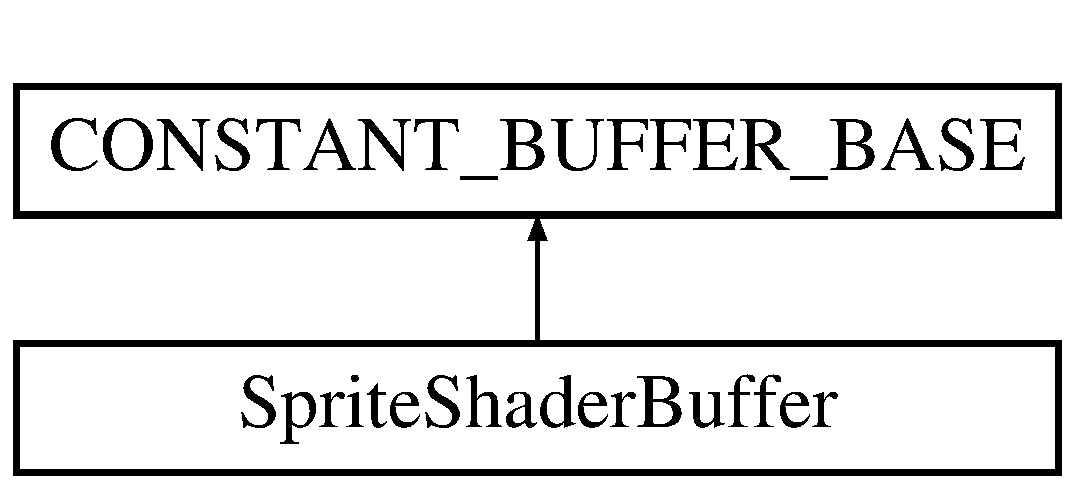
\includegraphics[height=2.000000cm]{struct_d3_d11_1_1_graphic_1_1_sprite_shader_buffer}
\end{center}
\end{figure}
\subsection*{公開変数類}
\begin{DoxyCompactItemize}
\item 
\hyperlink{struct_d3_d11_1_1_graphic_1_1_c_o_n_s_t_a_n_t___b_u_f_f_e_r___b_a_s_e_a3443b7ba28a2ff538b5d9f5f82c02b55}{A\+L\+I\+G\+N16}$<$ Direct\+X\+::\+X\+M\+F\+L\+O\+A\+T2 $>$ {\bfseries m\+\_\+\+Div\+Num}\hypertarget{struct_d3_d11_1_1_graphic_1_1_sprite_shader_buffer_ac9aa37de1e2292c08d763df5e3255d68}{}\label{struct_d3_d11_1_1_graphic_1_1_sprite_shader_buffer_ac9aa37de1e2292c08d763df5e3255d68}

\item 
\hyperlink{struct_d3_d11_1_1_graphic_1_1_c_o_n_s_t_a_n_t___b_u_f_f_e_r___b_a_s_e_a3443b7ba28a2ff538b5d9f5f82c02b55}{A\+L\+I\+G\+N16}$<$ Direct\+X\+::\+X\+M\+F\+L\+O\+A\+T2 $>$ {\bfseries m\+\_\+\+Index}\hypertarget{struct_d3_d11_1_1_graphic_1_1_sprite_shader_buffer_a9b891fd9718c340c005376426d8f3ed0}{}\label{struct_d3_d11_1_1_graphic_1_1_sprite_shader_buffer_a9b891fd9718c340c005376426d8f3ed0}

\item 
\hyperlink{struct_d3_d11_1_1_graphic_1_1_c_o_n_s_t_a_n_t___b_u_f_f_e_r___b_a_s_e_a3443b7ba28a2ff538b5d9f5f82c02b55}{A\+L\+I\+G\+N16}$<$ Direct\+X\+::\+X\+M\+F\+L\+O\+A\+T4 $>$ {\bfseries m\+\_\+\+Color}\hypertarget{struct_d3_d11_1_1_graphic_1_1_sprite_shader_buffer_a90918a276359954b761522f699d958c5}{}\label{struct_d3_d11_1_1_graphic_1_1_sprite_shader_buffer_a90918a276359954b761522f699d958c5}

\end{DoxyCompactItemize}
\subsection*{その他の継承メンバ}


\subsection{詳解}
スプライトのコンスタントバッファ構造体 

この構造体詳解は次のファイルから抽出されました\+:\begin{DoxyCompactItemize}
\item 
C\+:/\+Users/yuuki/\+Desktop/\+Doxygen\+\_\+lib\+\_\+source/include/Sprite.\+h\end{DoxyCompactItemize}

\hypertarget{struct_d3_d11_1_1_graphic_1_1_sprite_vertex}{}\section{Sprite\+Vertex 構造体}
\label{struct_d3_d11_1_1_graphic_1_1_sprite_vertex}\index{Sprite\+Vertex@{Sprite\+Vertex}}


スプライトの頂点構造体  




{\ttfamily \#include $<$Sprite.\+h$>$}

Sprite\+Vertex の継承関係図\begin{figure}[H]
\begin{center}
\leavevmode
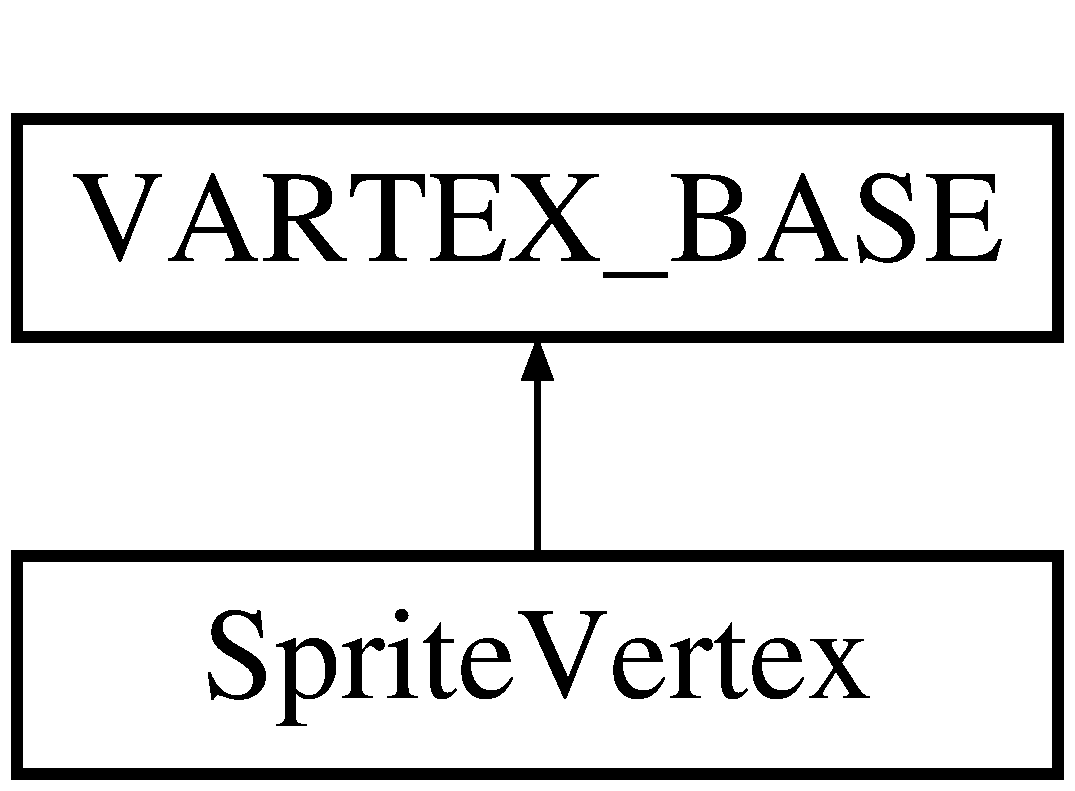
\includegraphics[height=2.000000cm]{struct_d3_d11_1_1_graphic_1_1_sprite_vertex}
\end{center}
\end{figure}
\subsection*{公開メンバ関数}
\begin{DoxyCompactItemize}
\item 
{\bfseries Sprite\+Vertex} (Direct\+X\+::\+X\+M\+F\+L\+O\+A\+T3 pos, Direct\+X\+::\+X\+M\+F\+L\+O\+A\+T2 uv)\hypertarget{struct_d3_d11_1_1_graphic_1_1_sprite_vertex_a24107e65f29cc3aa3127346b1cd6c7e4}{}\label{struct_d3_d11_1_1_graphic_1_1_sprite_vertex_a24107e65f29cc3aa3127346b1cd6c7e4}

\end{DoxyCompactItemize}
\subsection*{公開変数類}
\begin{DoxyCompactItemize}
\item 
Direct\+X\+::\+X\+M\+F\+L\+O\+A\+T2 {\bfseries m\+\_\+\+UV}\hypertarget{struct_d3_d11_1_1_graphic_1_1_sprite_vertex_a4b3ceaf10dd4b638b7afed185e03cdff}{}\label{struct_d3_d11_1_1_graphic_1_1_sprite_vertex_a4b3ceaf10dd4b638b7afed185e03cdff}

\end{DoxyCompactItemize}


\subsection{詳解}
スプライトの頂点構造体 

この構造体詳解は次のファイルから抽出されました\+:\begin{DoxyCompactItemize}
\item 
C\+:/\+Users/yuuki/\+Desktop/\+Doxygen\+\_\+lib\+\_\+source/include/Sprite.\+h\end{DoxyCompactItemize}

\hypertarget{class_a_p_i_1_1_texture}{}\section{Texture クラス}
\label{class_a_p_i_1_1_texture}\index{Texture@{Texture}}
Texture の継承関係図\begin{figure}[H]
\begin{center}
\leavevmode
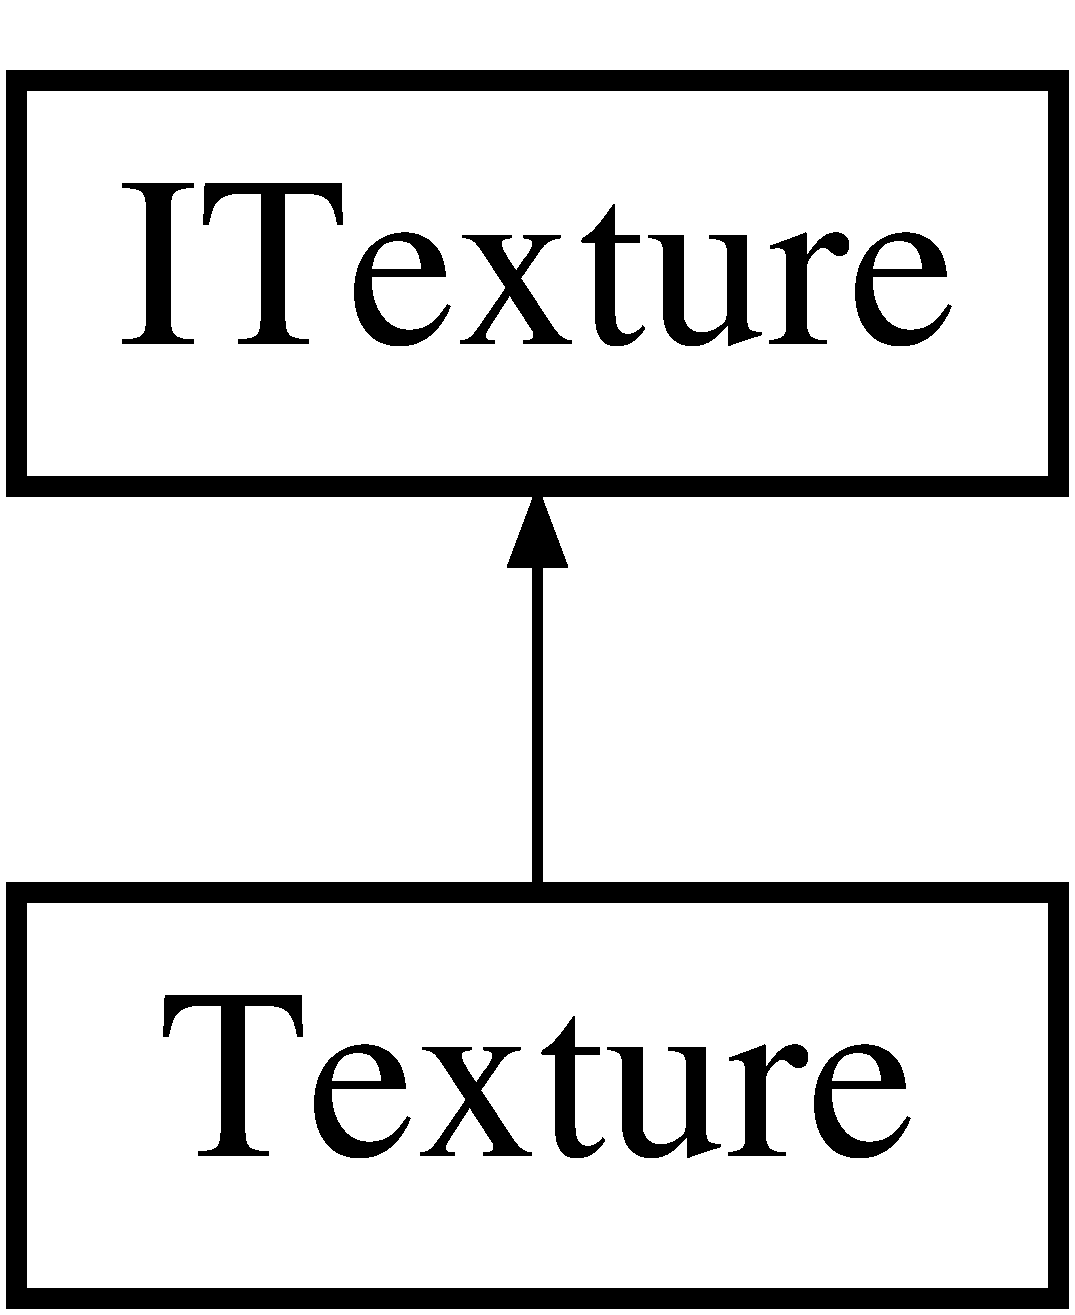
\includegraphics[height=2.000000cm]{class_a_p_i_1_1_texture}
\end{center}
\end{figure}
\subsection*{公開メンバ関数}
\begin{DoxyCompactItemize}
\item 
\hyperlink{class_a_p_i_1_1_texture_a5c292543baec1a3caa8a4ee3f19dbeb7}{Texture} ()
\begin{DoxyCompactList}\small\item\em コンストラクタ \end{DoxyCompactList}\item 
\hyperlink{class_a_p_i_1_1_texture_aa85421a8ef676058b4fb96337be881d1}{$\sim$\+Texture} () override
\begin{DoxyCompactList}\small\item\em デストラクタ \end{DoxyCompactList}\item 
H\+R\+E\+S\+U\+LT {\bfseries Initialize} (std\+::string file\+Path)\hypertarget{class_a_p_i_1_1_texture_a97a316fc5d1e3b552e48527f9204279e}{}\label{class_a_p_i_1_1_texture_a97a316fc5d1e3b552e48527f9204279e}

\item 
H\+R\+E\+S\+U\+LT {\bfseries Initialize} (std\+::string file\+Path, const Direct\+X\+::\+X\+M\+I\+N\+T2 size)\hypertarget{class_a_p_i_1_1_texture_a821bbb88db5bfcde14bc562b60e82bde}{}\label{class_a_p_i_1_1_texture_a821bbb88db5bfcde14bc562b60e82bde}

\item 
H\+R\+E\+S\+U\+LT {\bfseries Initialize} (std\+::string file\+Path, const Tile\+Mode tile\+Mode)\hypertarget{class_a_p_i_1_1_texture_a07c4f2bb1b604fd5bdff7f0ca707bed7}{}\label{class_a_p_i_1_1_texture_a07c4f2bb1b604fd5bdff7f0ca707bed7}

\item 
H\+R\+E\+S\+U\+LT {\bfseries Initialize} (std\+::string file\+Path, const Direct\+X\+::\+X\+M\+I\+N\+T2 size, const Tile\+Mode tile\+Mode)\hypertarget{class_a_p_i_1_1_texture_a8fdf4c49a054581490c3a5058b22ea01}{}\label{class_a_p_i_1_1_texture_a8fdf4c49a054581490c3a5058b22ea01}

\item 
H\+R\+E\+S\+U\+LT {\bfseries Initialize} (std\+::string file\+Path, const Filtering\+Mode filter\+Mode)\hypertarget{class_a_p_i_1_1_texture_ad651f579e1693532dcdb2d5b0554b0a4}{}\label{class_a_p_i_1_1_texture_ad651f579e1693532dcdb2d5b0554b0a4}

\item 
H\+R\+E\+S\+U\+LT {\bfseries Initialize} (std\+::string file\+Path, const Direct\+X\+::\+X\+M\+I\+N\+T2 size, const Filtering\+Mode filter\+Mode)\hypertarget{class_a_p_i_1_1_texture_a2129e4ccc0830c8b4e74c44ef486cf5d}{}\label{class_a_p_i_1_1_texture_a2129e4ccc0830c8b4e74c44ef486cf5d}

\item 
H\+R\+E\+S\+U\+LT \hyperlink{class_a_p_i_1_1_texture_af698b21cca64ab6b34e9c6573bb4a603}{Initialize} (std\+::string file\+Path, const Tile\+Mode tile\+Mode, const Filtering\+Mode filter\+Mode)
\item 
H\+R\+E\+S\+U\+LT \hyperlink{class_a_p_i_1_1_texture_ab3c22087751cc64c33cfb4dc10a00720}{Initialize} (std\+::string file\+Path, const Direct\+X\+::\+X\+M\+I\+N\+T2 size, const Tile\+Mode tile\+Mode, const Filtering\+Mode filter\+Mode)
\item 
void \hyperlink{class_a_p_i_1_1_texture_aadf4b965bdac3ac366a8fbe876509fcb}{Finalize} () override
\end{DoxyCompactItemize}


\subsection{構築子と解体子}
\index{A\+P\+I\+::\+Texture@{A\+P\+I\+::\+Texture}!Texture@{Texture}}
\index{Texture@{Texture}!A\+P\+I\+::\+Texture@{A\+P\+I\+::\+Texture}}
\subsubsection[{\texorpdfstring{Texture()}{Texture()}}]{\setlength{\rightskip}{0pt plus 5cm}{\bf Texture} (
\begin{DoxyParamCaption}
{}
\end{DoxyParamCaption}
)\hspace{0.3cm}{\ttfamily [explicit]}}\hypertarget{class_a_p_i_1_1_texture_a5c292543baec1a3caa8a4ee3f19dbeb7}{}\label{class_a_p_i_1_1_texture_a5c292543baec1a3caa8a4ee3f19dbeb7}


コンストラクタ 

コンストラクタ  生成時に\+I\+Textureのコンストラクタを呼び出しデフォルト値を入れる \index{A\+P\+I\+::\+Texture@{A\+P\+I\+::\+Texture}!````~Texture@{$\sim$\+Texture}}
\index{````~Texture@{$\sim$\+Texture}!A\+P\+I\+::\+Texture@{A\+P\+I\+::\+Texture}}
\subsubsection[{\texorpdfstring{$\sim$\+Texture() override}{~Texture() override}}]{\setlength{\rightskip}{0pt plus 5cm}$\sim${\bf Texture} (
\begin{DoxyParamCaption}
{}
\end{DoxyParamCaption}
)\hspace{0.3cm}{\ttfamily [override]}}\hypertarget{class_a_p_i_1_1_texture_aa85421a8ef676058b4fb96337be881d1}{}\label{class_a_p_i_1_1_texture_aa85421a8ef676058b4fb96337be881d1}


デストラクタ 

デストラクタ  Finalize呼び出し 

\subsection{関数詳解}
\index{A\+P\+I\+::\+Texture@{A\+P\+I\+::\+Texture}!Finalize@{Finalize}}
\index{Finalize@{Finalize}!A\+P\+I\+::\+Texture@{A\+P\+I\+::\+Texture}}
\subsubsection[{\texorpdfstring{Finalize() override}{Finalize() override}}]{\setlength{\rightskip}{0pt plus 5cm}void Finalize (
\begin{DoxyParamCaption}
{}
\end{DoxyParamCaption}
)\hspace{0.3cm}{\ttfamily [override]}}\hypertarget{class_a_p_i_1_1_texture_aadf4b965bdac3ac366a8fbe876509fcb}{}\label{class_a_p_i_1_1_texture_aadf4b965bdac3ac366a8fbe876509fcb}
抽象クラスのメンバの破棄 \index{A\+P\+I\+::\+Texture@{A\+P\+I\+::\+Texture}!Initialize@{Initialize}}
\index{Initialize@{Initialize}!A\+P\+I\+::\+Texture@{A\+P\+I\+::\+Texture}}
\subsubsection[{\texorpdfstring{Initialize(std\+::string file\+Path, const Tile\+Mode tile\+Mode, const Filtering\+Mode filter\+Mode)}{Initialize(std::string filePath, const TileMode tileMode, const FilteringMode filterMode)}}]{\setlength{\rightskip}{0pt plus 5cm}H\+R\+E\+S\+U\+LT Initialize (
\begin{DoxyParamCaption}
\item[{std\+::string}]{file\+Path, }
\item[{const Tile\+Mode}]{tile\+Mode, }
\item[{const Filtering\+Mode}]{filter\+Mode}
\end{DoxyParamCaption}
)}\hypertarget{class_a_p_i_1_1_texture_af698b21cca64ab6b34e9c6573bb4a603}{}\label{class_a_p_i_1_1_texture_af698b21cca64ab6b34e9c6573bb4a603}
画像のロード

タイリングモード

フィルタリングモード

タイリングとフィルタリングを設定し、サンプラーステートを作成 \index{A\+P\+I\+::\+Texture@{A\+P\+I\+::\+Texture}!Initialize@{Initialize}}
\index{Initialize@{Initialize}!A\+P\+I\+::\+Texture@{A\+P\+I\+::\+Texture}}
\subsubsection[{\texorpdfstring{Initialize(std\+::string file\+Path, const Direct\+X\+::\+X\+M\+I\+N\+T2 size, const Tile\+Mode tile\+Mode, const Filtering\+Mode filter\+Mode)}{Initialize(std::string filePath, const DirectX::XMINT2 size, const TileMode tileMode, const FilteringMode filterMode)}}]{\setlength{\rightskip}{0pt plus 5cm}H\+R\+E\+S\+U\+LT Initialize (
\begin{DoxyParamCaption}
\item[{std\+::string}]{file\+Path, }
\item[{const Direct\+X\+::\+X\+M\+I\+N\+T2}]{size, }
\item[{const Tile\+Mode}]{tile\+Mode, }
\item[{const Filtering\+Mode}]{filter\+Mode}
\end{DoxyParamCaption}
)}\hypertarget{class_a_p_i_1_1_texture_ab3c22087751cc64c33cfb4dc10a00720}{}\label{class_a_p_i_1_1_texture_ab3c22087751cc64c33cfb4dc10a00720}
初期化

サイズの設定 

このクラス詳解は次のファイルから抽出されました\+:\begin{DoxyCompactItemize}
\item 
C\+:/\+Users/yuuki/\+Desktop/\+Doxygen\+\_\+lib\+\_\+source/include/Texture.\+h\item 
C\+:/\+Users/yuuki/\+Desktop/\+Doxygen\+\_\+lib\+\_\+source/include/Texture.\+cpp\end{DoxyCompactItemize}

\hypertarget{class_a_p_i_1_1_texture_atlas}{}\section{Texture\+Atlas クラス}
\label{class_a_p_i_1_1_texture_atlas}\index{Texture\+Atlas@{Texture\+Atlas}}
Texture\+Atlas の継承関係図\begin{figure}[H]
\begin{center}
\leavevmode
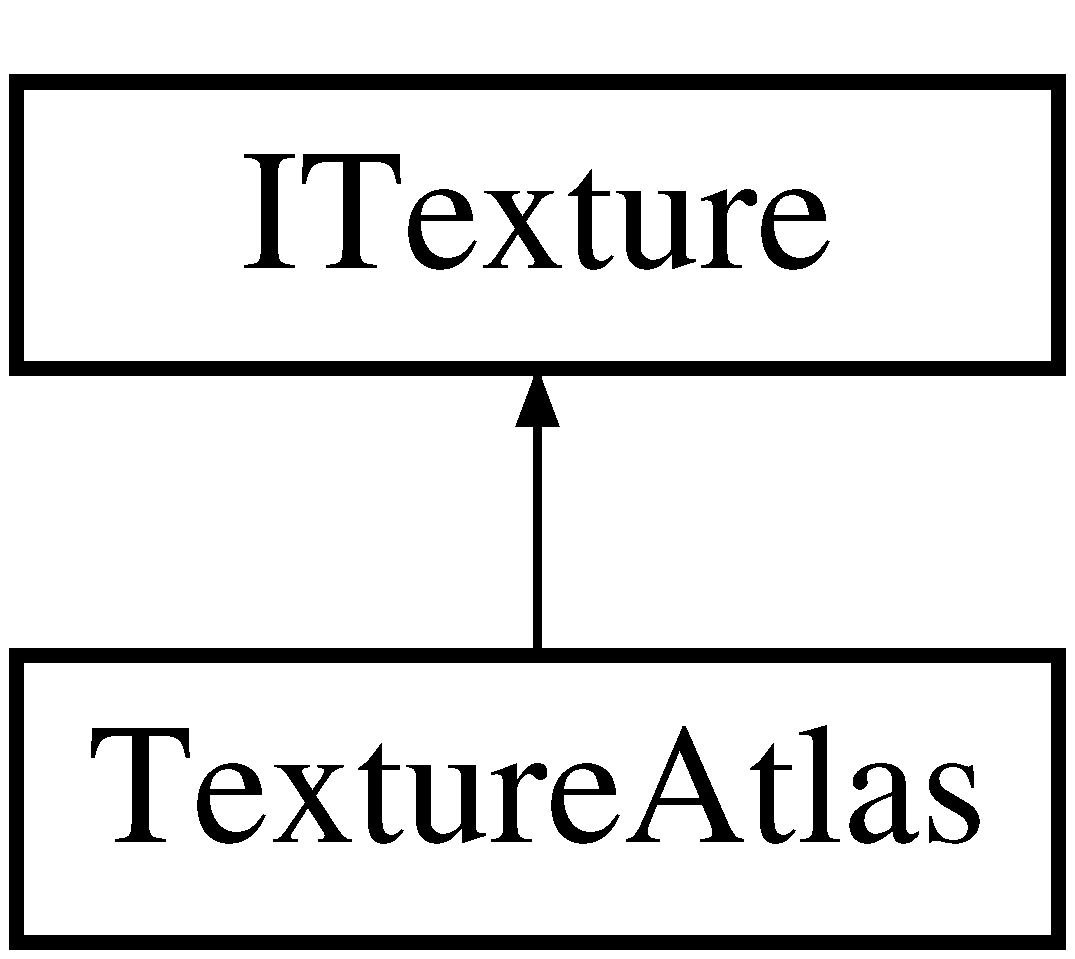
\includegraphics[height=2.000000cm]{class_a_p_i_1_1_texture_atlas}
\end{center}
\end{figure}
\subsection*{公開メンバ関数}
\begin{DoxyCompactItemize}
\item 
\hyperlink{class_a_p_i_1_1_texture_atlas_a200db7ac91cea63c9f454a01780b68df}{Texture\+Atlas} ()
\begin{DoxyCompactList}\small\item\em コンストラクタ \end{DoxyCompactList}\item 
\hyperlink{class_a_p_i_1_1_texture_atlas_afb13a479220b34cb7399c2f9be06336a}{$\sim$\+Texture\+Atlas} () override
\begin{DoxyCompactList}\small\item\em デストラクタ \end{DoxyCompactList}\item 
H\+R\+E\+S\+U\+LT {\bfseries Initialize} (std\+::string file\+Path, const Direct\+X\+::\+X\+M\+F\+L\+O\+A\+T2 div\+Num)\hypertarget{class_a_p_i_1_1_texture_atlas_ac9d8323342b75d22e90a27ed4cdc49e7}{}\label{class_a_p_i_1_1_texture_atlas_ac9d8323342b75d22e90a27ed4cdc49e7}

\item 
H\+R\+E\+S\+U\+LT \hyperlink{class_a_p_i_1_1_texture_atlas_a31953216d036affed2f1f601d99a269f}{Initialize} (std\+::string file\+Path, const Direct\+X\+::\+X\+M\+I\+N\+T2 size, const Direct\+X\+::\+X\+M\+F\+L\+O\+A\+T2 div\+Num)
\item 
H\+R\+E\+S\+U\+LT {\bfseries Initialize} (std\+::string file\+Path, const Direct\+X\+::\+X\+M\+F\+L\+O\+A\+T2 div\+Num, const Filtering\+Mode filter\+Mode)\hypertarget{class_a_p_i_1_1_texture_atlas_a828dcc3d5825d3f915e0383fe872ce5f}{}\label{class_a_p_i_1_1_texture_atlas_a828dcc3d5825d3f915e0383fe872ce5f}

\item 
H\+R\+E\+S\+U\+LT \hyperlink{class_a_p_i_1_1_texture_atlas_ae9b214a35ca6e19e83727006147c73cf}{Initialize} (std\+::string file\+Path, const Direct\+X\+::\+X\+M\+I\+N\+T2 size, const Direct\+X\+::\+X\+M\+F\+L\+O\+A\+T2 div\+Num, const Filtering\+Mode filter\+Mode)
\item 
void \hyperlink{class_a_p_i_1_1_texture_atlas_aadf4b965bdac3ac366a8fbe876509fcb}{Finalize} () override
\item 
void {\bfseries Set\+Dev\+Num} (const Direct\+X\+::\+X\+M\+F\+L\+O\+A\+T2 div\+Num)\hypertarget{class_a_p_i_1_1_texture_atlas_a6eea55cb7fee63b28622bf3bde439570}{}\label{class_a_p_i_1_1_texture_atlas_a6eea55cb7fee63b28622bf3bde439570}

\item 
void {\bfseries Set\+Atlas\+Index} (const Direct\+X\+::\+X\+M\+F\+L\+O\+A\+T2 index)\hypertarget{class_a_p_i_1_1_texture_atlas_a936129d1cf73f242c5e74f7b87be9168}{}\label{class_a_p_i_1_1_texture_atlas_a936129d1cf73f242c5e74f7b87be9168}

\item 
Direct\+X\+::\+X\+M\+F\+L\+O\+A\+T2 {\bfseries Get\+Div\+Num} () const \hypertarget{class_a_p_i_1_1_texture_atlas_ad95b8474f02c2100d2149ddbc85ba456}{}\label{class_a_p_i_1_1_texture_atlas_ad95b8474f02c2100d2149ddbc85ba456}

\item 
Direct\+X\+::\+X\+M\+F\+L\+O\+A\+T2 {\bfseries Get\+Atlas\+Index} () const \hypertarget{class_a_p_i_1_1_texture_atlas_ad20c9565d1aa6ca8b9a78ba50baaedc9}{}\label{class_a_p_i_1_1_texture_atlas_ad20c9565d1aa6ca8b9a78ba50baaedc9}

\end{DoxyCompactItemize}
\subsection*{非公開メンバ関数}
\begin{DoxyCompactItemize}
\item 
H\+R\+E\+S\+U\+LT \hyperlink{class_a_p_i_1_1_texture_atlas_aa4937eaead1a57cbf5bbc926adf01b23}{Initialize} (std\+::string file\+Path, const Direct\+X\+::\+X\+M\+I\+N\+T2 size, const Direct\+X\+::\+X\+M\+F\+L\+O\+A\+T2 div\+Num, const Tile\+Mode tile\+Mode, const Filtering\+Mode filter\+Mode)
\item 
H\+R\+E\+S\+U\+LT \hyperlink{class_a_p_i_1_1_texture_atlas_a50471fd5a53358b68143e27c2c3107e0}{Initialize} (std\+::string file\+Path, const Direct\+X\+::\+X\+M\+F\+L\+O\+A\+T2 div\+Num, const Tile\+Mode tile\+Mode, const Filtering\+Mode filter\+Mode)
\end{DoxyCompactItemize}
\subsection*{非公開変数類}
\begin{DoxyCompactItemize}
\item 
Direct\+X\+::\+X\+M\+F\+L\+O\+A\+T2 \hyperlink{class_a_p_i_1_1_texture_atlas_aa7382d61a1bd4e726d8f2730e07d92ed}{m\+\_\+\+Div\+Num}
\item 
Direct\+X\+::\+X\+M\+F\+L\+O\+A\+T2 \hyperlink{class_a_p_i_1_1_texture_atlas_ade24c54e9200934a5852b874df6bfaaf}{m\+\_\+\+Index}
\end{DoxyCompactItemize}


\subsection{構築子と解体子}
\index{A\+P\+I\+::\+Texture\+Atlas@{A\+P\+I\+::\+Texture\+Atlas}!Texture\+Atlas@{Texture\+Atlas}}
\index{Texture\+Atlas@{Texture\+Atlas}!A\+P\+I\+::\+Texture\+Atlas@{A\+P\+I\+::\+Texture\+Atlas}}
\subsubsection[{\texorpdfstring{Texture\+Atlas()}{TextureAtlas()}}]{\setlength{\rightskip}{0pt plus 5cm}{\bf Texture\+Atlas} (
\begin{DoxyParamCaption}
{}
\end{DoxyParamCaption}
)\hspace{0.3cm}{\ttfamily [explicit]}}\hypertarget{class_a_p_i_1_1_texture_atlas_a200db7ac91cea63c9f454a01780b68df}{}\label{class_a_p_i_1_1_texture_atlas_a200db7ac91cea63c9f454a01780b68df}


コンストラクタ 

コンストラクタ  生成時に\+I\+Textureのコンストラクタを呼び出しデフォルト値を入れる 分割数は描画前に設定されていることが前提なのでデフォルトでは参照外を設定しておく。 逆にインデックスは指定なしでも描画できるように分割したした際の最小値を設定しておく \index{A\+P\+I\+::\+Texture\+Atlas@{A\+P\+I\+::\+Texture\+Atlas}!````~Texture\+Atlas@{$\sim$\+Texture\+Atlas}}
\index{````~Texture\+Atlas@{$\sim$\+Texture\+Atlas}!A\+P\+I\+::\+Texture\+Atlas@{A\+P\+I\+::\+Texture\+Atlas}}
\subsubsection[{\texorpdfstring{$\sim$\+Texture\+Atlas() override}{~TextureAtlas() override}}]{\setlength{\rightskip}{0pt plus 5cm}$\sim${\bf Texture\+Atlas} (
\begin{DoxyParamCaption}
{}
\end{DoxyParamCaption}
)\hspace{0.3cm}{\ttfamily [override]}}\hypertarget{class_a_p_i_1_1_texture_atlas_afb13a479220b34cb7399c2f9be06336a}{}\label{class_a_p_i_1_1_texture_atlas_afb13a479220b34cb7399c2f9be06336a}


デストラクタ 

デストラクタ  Finalize呼び出し 

\subsection{関数詳解}
\index{A\+P\+I\+::\+Texture\+Atlas@{A\+P\+I\+::\+Texture\+Atlas}!Finalize@{Finalize}}
\index{Finalize@{Finalize}!A\+P\+I\+::\+Texture\+Atlas@{A\+P\+I\+::\+Texture\+Atlas}}
\subsubsection[{\texorpdfstring{Finalize() override}{Finalize() override}}]{\setlength{\rightskip}{0pt plus 5cm}void Finalize (
\begin{DoxyParamCaption}
{}
\end{DoxyParamCaption}
)\hspace{0.3cm}{\ttfamily [override]}}\hypertarget{class_a_p_i_1_1_texture_atlas_aadf4b965bdac3ac366a8fbe876509fcb}{}\label{class_a_p_i_1_1_texture_atlas_aadf4b965bdac3ac366a8fbe876509fcb}
抽象クラスのメンバの破棄 \index{A\+P\+I\+::\+Texture\+Atlas@{A\+P\+I\+::\+Texture\+Atlas}!Initialize@{Initialize}}
\index{Initialize@{Initialize}!A\+P\+I\+::\+Texture\+Atlas@{A\+P\+I\+::\+Texture\+Atlas}}
\subsubsection[{\texorpdfstring{Initialize(std\+::string file\+Path, const Direct\+X\+::\+X\+M\+I\+N\+T2 size, const Direct\+X\+::\+X\+M\+F\+L\+O\+A\+T2 div\+Num)}{Initialize(std::string filePath, const DirectX::XMINT2 size, const DirectX::XMFLOAT2 divNum)}}]{\setlength{\rightskip}{0pt plus 5cm}H\+R\+E\+S\+U\+LT Initialize (
\begin{DoxyParamCaption}
\item[{std\+::string}]{file\+Path, }
\item[{const Direct\+X\+::\+X\+M\+I\+N\+T2}]{size, }
\item[{const Direct\+X\+::\+X\+M\+F\+L\+O\+A\+T2}]{div\+Num}
\end{DoxyParamCaption}
)}\hypertarget{class_a_p_i_1_1_texture_atlas_a31953216d036affed2f1f601d99a269f}{}\label{class_a_p_i_1_1_texture_atlas_a31953216d036affed2f1f601d99a269f}
初期化

サイズの設定 \index{A\+P\+I\+::\+Texture\+Atlas@{A\+P\+I\+::\+Texture\+Atlas}!Initialize@{Initialize}}
\index{Initialize@{Initialize}!A\+P\+I\+::\+Texture\+Atlas@{A\+P\+I\+::\+Texture\+Atlas}}
\subsubsection[{\texorpdfstring{Initialize(std\+::string file\+Path, const Direct\+X\+::\+X\+M\+I\+N\+T2 size, const Direct\+X\+::\+X\+M\+F\+L\+O\+A\+T2 div\+Num, const Filtering\+Mode filter\+Mode)}{Initialize(std::string filePath, const DirectX::XMINT2 size, const DirectX::XMFLOAT2 divNum, const FilteringMode filterMode)}}]{\setlength{\rightskip}{0pt plus 5cm}H\+R\+E\+S\+U\+LT Initialize (
\begin{DoxyParamCaption}
\item[{std\+::string}]{file\+Path, }
\item[{const Direct\+X\+::\+X\+M\+I\+N\+T2}]{size, }
\item[{const Direct\+X\+::\+X\+M\+F\+L\+O\+A\+T2}]{div\+Num, }
\item[{const Filtering\+Mode}]{filter\+Mode}
\end{DoxyParamCaption}
)}\hypertarget{class_a_p_i_1_1_texture_atlas_ae9b214a35ca6e19e83727006147c73cf}{}\label{class_a_p_i_1_1_texture_atlas_ae9b214a35ca6e19e83727006147c73cf}
初期化

サイズの設定 \index{A\+P\+I\+::\+Texture\+Atlas@{A\+P\+I\+::\+Texture\+Atlas}!Initialize@{Initialize}}
\index{Initialize@{Initialize}!A\+P\+I\+::\+Texture\+Atlas@{A\+P\+I\+::\+Texture\+Atlas}}
\subsubsection[{\texorpdfstring{Initialize(std\+::string file\+Path, const Direct\+X\+::\+X\+M\+I\+N\+T2 size, const Direct\+X\+::\+X\+M\+F\+L\+O\+A\+T2 div\+Num, const Tile\+Mode tile\+Mode, const Filtering\+Mode filter\+Mode)}{Initialize(std::string filePath, const DirectX::XMINT2 size, const DirectX::XMFLOAT2 divNum, const TileMode tileMode, const FilteringMode filterMode)}}]{\setlength{\rightskip}{0pt plus 5cm}H\+R\+E\+S\+U\+LT Initialize (
\begin{DoxyParamCaption}
\item[{std\+::string}]{file\+Path, }
\item[{const Direct\+X\+::\+X\+M\+I\+N\+T2}]{size, }
\item[{const Direct\+X\+::\+X\+M\+F\+L\+O\+A\+T2}]{div\+Num, }
\item[{const Tile\+Mode}]{tile\+Mode, }
\item[{const Filtering\+Mode}]{filter\+Mode}
\end{DoxyParamCaption}
)\hspace{0.3cm}{\ttfamily [private]}}\hypertarget{class_a_p_i_1_1_texture_atlas_aa4937eaead1a57cbf5bbc926adf01b23}{}\label{class_a_p_i_1_1_texture_atlas_aa4937eaead1a57cbf5bbc926adf01b23}
画像のロード

タイリングモード

フィルタリングモード

タイリングとフィルタリングを設定し、サンプラーステートを作成

分割数の設定

サイズの設定 \index{A\+P\+I\+::\+Texture\+Atlas@{A\+P\+I\+::\+Texture\+Atlas}!Initialize@{Initialize}}
\index{Initialize@{Initialize}!A\+P\+I\+::\+Texture\+Atlas@{A\+P\+I\+::\+Texture\+Atlas}}
\subsubsection[{\texorpdfstring{Initialize(std\+::string file\+Path, const Direct\+X\+::\+X\+M\+F\+L\+O\+A\+T2 div\+Num, const Tile\+Mode tile\+Mode, const Filtering\+Mode filter\+Mode)}{Initialize(std::string filePath, const DirectX::XMFLOAT2 divNum, const TileMode tileMode, const FilteringMode filterMode)}}]{\setlength{\rightskip}{0pt plus 5cm}H\+R\+E\+S\+U\+LT Initialize (
\begin{DoxyParamCaption}
\item[{std\+::string}]{file\+Path, }
\item[{const Direct\+X\+::\+X\+M\+F\+L\+O\+A\+T2}]{div\+Num, }
\item[{const Tile\+Mode}]{tile\+Mode, }
\item[{const Filtering\+Mode}]{filter\+Mode}
\end{DoxyParamCaption}
)\hspace{0.3cm}{\ttfamily [private]}}\hypertarget{class_a_p_i_1_1_texture_atlas_a50471fd5a53358b68143e27c2c3107e0}{}\label{class_a_p_i_1_1_texture_atlas_a50471fd5a53358b68143e27c2c3107e0}
画像のロード

タイリングモード

フィルタリングモード

タイリングとフィルタリングを設定し、サンプラーステートを作成

分割数の設定 

\subsection{メンバ詳解}
\index{A\+P\+I\+::\+Texture\+Atlas@{A\+P\+I\+::\+Texture\+Atlas}!m\+\_\+\+Div\+Num@{m\+\_\+\+Div\+Num}}
\index{m\+\_\+\+Div\+Num@{m\+\_\+\+Div\+Num}!A\+P\+I\+::\+Texture\+Atlas@{A\+P\+I\+::\+Texture\+Atlas}}
\subsubsection[{\texorpdfstring{m\+\_\+\+Div\+Num}{m_DivNum}}]{\setlength{\rightskip}{0pt plus 5cm}Direct\+X\+::\+X\+M\+F\+L\+O\+A\+T2 m\+\_\+\+Div\+Num\hspace{0.3cm}{\ttfamily [private]}}\hypertarget{class_a_p_i_1_1_texture_atlas_aa7382d61a1bd4e726d8f2730e07d92ed}{}\label{class_a_p_i_1_1_texture_atlas_aa7382d61a1bd4e726d8f2730e07d92ed}
分割数 \index{A\+P\+I\+::\+Texture\+Atlas@{A\+P\+I\+::\+Texture\+Atlas}!m\+\_\+\+Index@{m\+\_\+\+Index}}
\index{m\+\_\+\+Index@{m\+\_\+\+Index}!A\+P\+I\+::\+Texture\+Atlas@{A\+P\+I\+::\+Texture\+Atlas}}
\subsubsection[{\texorpdfstring{m\+\_\+\+Index}{m_Index}}]{\setlength{\rightskip}{0pt plus 5cm}Direct\+X\+::\+X\+M\+F\+L\+O\+A\+T2 m\+\_\+\+Index\hspace{0.3cm}{\ttfamily [private]}}\hypertarget{class_a_p_i_1_1_texture_atlas_ade24c54e9200934a5852b874df6bfaaf}{}\label{class_a_p_i_1_1_texture_atlas_ade24c54e9200934a5852b874df6bfaaf}
描画するテクスチャ番号 

このクラス詳解は次のファイルから抽出されました\+:\begin{DoxyCompactItemize}
\item 
C\+:/\+Users/yuuki/\+Desktop/\+Doxygen\+\_\+lib\+\_\+source/include/Texture\+Atlas.\+h\item 
C\+:/\+Users/yuuki/\+Desktop/\+Doxygen\+\_\+lib\+\_\+source/include/Texture\+Atlas.\+cpp\end{DoxyCompactItemize}

\hypertarget{struct_d3_d11_1_1_graphic_1_1_v_a_r_t_e_x___b_a_s_e}{}\section{V\+A\+R\+T\+E\+X\+\_\+\+B\+A\+SE 構造体}
\label{struct_d3_d11_1_1_graphic_1_1_v_a_r_t_e_x___b_a_s_e}\index{V\+A\+R\+T\+E\+X\+\_\+\+B\+A\+SE@{V\+A\+R\+T\+E\+X\+\_\+\+B\+A\+SE}}


基底頂点構造体  




{\ttfamily \#include $<$Struct\+Shader\+Base.\+h$>$}

V\+A\+R\+T\+E\+X\+\_\+\+B\+A\+SE の継承関係図\begin{figure}[H]
\begin{center}
\leavevmode
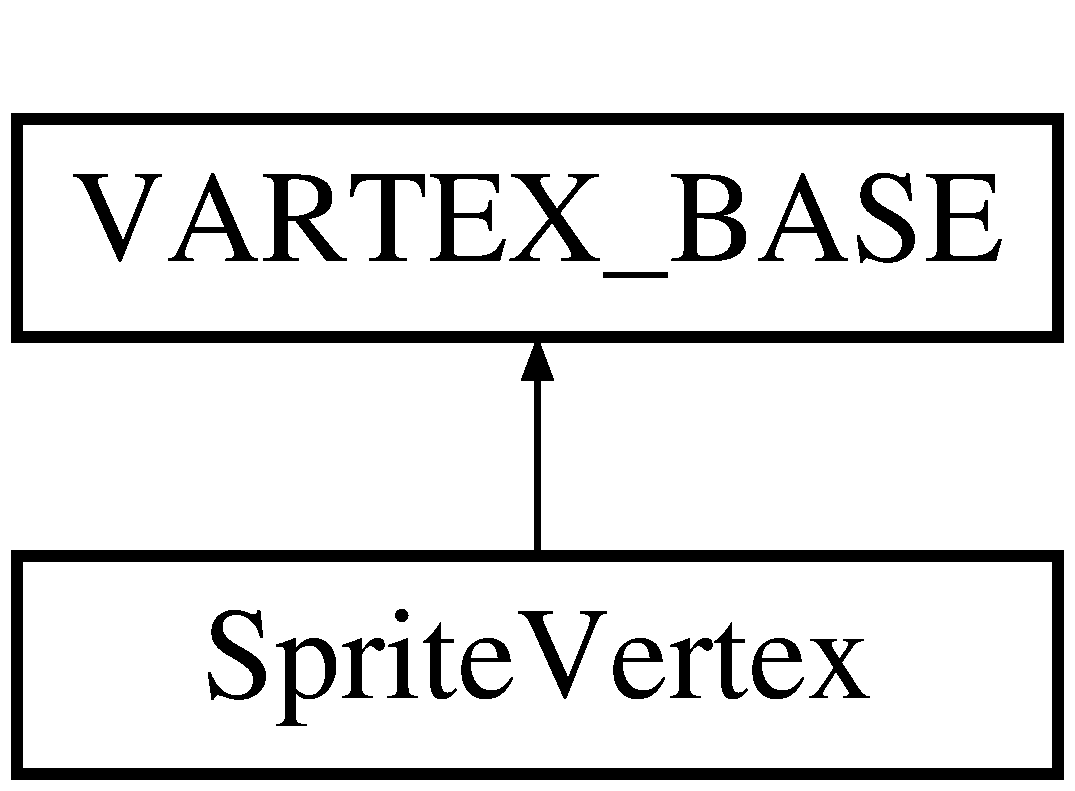
\includegraphics[height=2.000000cm]{struct_d3_d11_1_1_graphic_1_1_v_a_r_t_e_x___b_a_s_e}
\end{center}
\end{figure}
\subsection*{公開変数類}
\begin{DoxyCompactItemize}
\item 
Direct\+X\+::\+X\+M\+F\+L\+O\+A\+T3 {\bfseries m\+\_\+\+Pos}\hypertarget{struct_d3_d11_1_1_graphic_1_1_v_a_r_t_e_x___b_a_s_e_ac4dfe78085ef0a056c1ec0b18bbf894b}{}\label{struct_d3_d11_1_1_graphic_1_1_v_a_r_t_e_x___b_a_s_e_ac4dfe78085ef0a056c1ec0b18bbf894b}

\end{DoxyCompactItemize}


\subsection{詳解}
基底頂点構造体 

この構造体詳解は次のファイルから抽出されました\+:\begin{DoxyCompactItemize}
\item 
C\+:/\+Users/yuuki/\+Desktop/\+Doxygen\+\_\+lib\+\_\+source/include/Struct\+Shader\+Base.\+h\end{DoxyCompactItemize}

\hypertarget{class_a_p_i_1_1_wave}{}\section{Wave クラス}
\label{class_a_p_i_1_1_wave}\index{Wave@{Wave}}
\subsection*{公開メンバ関数}
\begin{DoxyCompactItemize}
\item 
\hyperlink{class_a_p_i_1_1_wave_a6fdcd896e9bbb4bc7dc1720dacacb1ed}{Wave} ()\hypertarget{class_a_p_i_1_1_wave_a6fdcd896e9bbb4bc7dc1720dacacb1ed}{}\label{class_a_p_i_1_1_wave_a6fdcd896e9bbb4bc7dc1720dacacb1ed}

\begin{DoxyCompactList}\small\item\em コンストラクタ \end{DoxyCompactList}\item 
\hyperlink{class_a_p_i_1_1_wave_a4cecd0f4bf1b520a3a3cddf626bafdcf}{$\sim$\+Wave} ()\hypertarget{class_a_p_i_1_1_wave_a4cecd0f4bf1b520a3a3cddf626bafdcf}{}\label{class_a_p_i_1_1_wave_a4cecd0f4bf1b520a3a3cddf626bafdcf}

\begin{DoxyCompactList}\small\item\em デストラクタ \end{DoxyCompactList}\item 
H\+R\+E\+S\+U\+LT {\bfseries Initialize} ()\hypertarget{class_a_p_i_1_1_wave_a81109341187e54cc3585f29a1306ca50}{}\label{class_a_p_i_1_1_wave_a81109341187e54cc3585f29a1306ca50}

\item 
void {\bfseries Finalize} ()\hypertarget{class_a_p_i_1_1_wave_a8fee61d7a783cade1a3d07fe86284d27}{}\label{class_a_p_i_1_1_wave_a8fee61d7a783cade1a3d07fe86284d27}

\item 
bool \hyperlink{class_a_p_i_1_1_wave_a70c8d413c8d0eeb72c33a58a3d9f2c02}{Load} (std\+::string file\+Path)
\item 
void \hyperlink{class_a_p_i_1_1_wave_a779405cdc18efe68b4c35846defa2278}{Play} (bool is\+Loop=false)
\item 
void {\bfseries Stop} ()\hypertarget{class_a_p_i_1_1_wave_a17a237457e57625296e6b24feb19c60a}{}\label{class_a_p_i_1_1_wave_a17a237457e57625296e6b24feb19c60a}

\item 
void {\bfseries Pause} ()\hypertarget{class_a_p_i_1_1_wave_a70babc5227ddd16ca31dccc6cec0bb22}{}\label{class_a_p_i_1_1_wave_a70babc5227ddd16ca31dccc6cec0bb22}

\item 
void \hyperlink{class_a_p_i_1_1_wave_a29aa2f1ad77425cf3079b275ed1a14c5}{Set\+Volume} (float vol)
\begin{DoxyCompactList}\small\item\em 音量変更  範囲 0〜1 \end{DoxyCompactList}\end{DoxyCompactItemize}
\subsection*{非公開変数類}
\begin{DoxyCompactItemize}
\item 
I\+X\+Audio2\+Source\+Voice $\ast$ {\bfseries m\+\_\+p\+Source\+Voice}\hypertarget{class_a_p_i_1_1_wave_ad98f819a0685ce72575781e2bb19e363}{}\label{class_a_p_i_1_1_wave_ad98f819a0685ce72575781e2bb19e363}

\item 
B\+Y\+TE $\ast$ {\bfseries m\+\_\+p\+Wave\+Buffer}\hypertarget{class_a_p_i_1_1_wave_af67d009b0241559c379599017fa20d20}{}\label{class_a_p_i_1_1_wave_af67d009b0241559c379599017fa20d20}

\item 
D\+W\+O\+RD {\bfseries m\+\_\+dw\+Wave\+Size}\hypertarget{class_a_p_i_1_1_wave_a22c820114efa9d6ed62ad7bfd494ea63}{}\label{class_a_p_i_1_1_wave_a22c820114efa9d6ed62ad7bfd494ea63}

\end{DoxyCompactItemize}


\subsection{関数詳解}
\index{A\+P\+I\+::\+Wave@{A\+P\+I\+::\+Wave}!Load@{Load}}
\index{Load@{Load}!A\+P\+I\+::\+Wave@{A\+P\+I\+::\+Wave}}
\subsubsection[{\texorpdfstring{Load(std\+::string file\+Path)}{Load(std::string filePath)}}]{\setlength{\rightskip}{0pt plus 5cm}bool Load (
\begin{DoxyParamCaption}
\item[{std\+::string}]{file\+Path}
\end{DoxyParamCaption}
)}\hypertarget{class_a_p_i_1_1_wave_a70c8d413c8d0eeb72c33a58a3d9f2c02}{}\label{class_a_p_i_1_1_wave_a70c8d413c8d0eeb72c33a58a3d9f2c02}
$<$ Windowsマルチメディア\+A\+P\+Iハンドル

$<$ Waveデータサイズ

$<$ Waveフォーマット

$<$ チャンク情報

$<$ 最上部チャンク

$<$ P\+C\+Mフォーマット

Waveファイル内のヘッダー情報読み込み

Waveファイルの読み込み失敗

ファイルポインタを\+R\+I\+F\+Fチャンクの先頭にセット

ファイルポインタを\textquotesingle{}f\textquotesingle{} \textquotesingle{}m\textquotesingle{} \textquotesingle{}t\textquotesingle{} \textquotesingle{} \textquotesingle{} チャンクにセットする

フォーマット読み込み

音データ読み込み

オーディオデバイスの参照

ソースボイスにデータ詰め込み

ソースボイス作成 \index{A\+P\+I\+::\+Wave@{A\+P\+I\+::\+Wave}!Play@{Play}}
\index{Play@{Play}!A\+P\+I\+::\+Wave@{A\+P\+I\+::\+Wave}}
\subsubsection[{\texorpdfstring{Play(bool is\+Loop=false)}{Play(bool isLoop=false)}}]{\setlength{\rightskip}{0pt plus 5cm}void Play (
\begin{DoxyParamCaption}
\item[{bool}]{is\+Loop = {\ttfamily false}}
\end{DoxyParamCaption}
)}\hypertarget{class_a_p_i_1_1_wave_a779405cdc18efe68b4c35846defa2278}{}\label{class_a_p_i_1_1_wave_a779405cdc18efe68b4c35846defa2278}
サブミット

$<$ 再生されるバッファの最初のサンプル

$<$ サウンドのバッファ全て \index{A\+P\+I\+::\+Wave@{A\+P\+I\+::\+Wave}!Set\+Volume@{Set\+Volume}}
\index{Set\+Volume@{Set\+Volume}!A\+P\+I\+::\+Wave@{A\+P\+I\+::\+Wave}}
\subsubsection[{\texorpdfstring{Set\+Volume(float vol)}{SetVolume(float vol)}}]{\setlength{\rightskip}{0pt plus 5cm}void Set\+Volume (
\begin{DoxyParamCaption}
\item[{float}]{vol}
\end{DoxyParamCaption}
)}\hypertarget{class_a_p_i_1_1_wave_a29aa2f1ad77425cf3079b275ed1a14c5}{}\label{class_a_p_i_1_1_wave_a29aa2f1ad77425cf3079b275ed1a14c5}


音量変更  範囲 0〜1 


\begin{DoxyParams}[1]{引数}
\mbox{\tt in}  & {\em 設定する音量} & \\
\hline
\end{DoxyParams}


このクラス詳解は次のファイルから抽出されました\+:\begin{DoxyCompactItemize}
\item 
C\+:/\+Users/yuuki/\+Desktop/\+Doxygen\+\_\+lib\+\_\+source/include/Wave.\+h\item 
C\+:/\+Users/yuuki/\+Desktop/\+Doxygen\+\_\+lib\+\_\+source/include/Wave.\+cpp\end{DoxyCompactItemize}

\hypertarget{class_window}{}\section{Window クラス}
\label{class_window}\index{Window@{Window}}
\subsection*{公開メンバ関数}
\begin{DoxyCompactItemize}
\item 
\hyperlink{class_window_a6cbfa660b1af1f7020fc63dce78aabad}{Window} ()=default\hypertarget{class_window_a6cbfa660b1af1f7020fc63dce78aabad}{}\label{class_window_a6cbfa660b1af1f7020fc63dce78aabad}

\begin{DoxyCompactList}\small\item\em コンストラクタ \end{DoxyCompactList}\item 
\hyperlink{class_window_a254ab61160c1cd5eaa46cc0475bb7a06}{$\sim$\+Window} ()\hypertarget{class_window_a254ab61160c1cd5eaa46cc0475bb7a06}{}\label{class_window_a254ab61160c1cd5eaa46cc0475bb7a06}

\begin{DoxyCompactList}\small\item\em デストラクタ \end{DoxyCompactList}\item 
L\+R\+E\+S\+U\+LT \hyperlink{class_window_ad4efa5601904d6c96a9411aadd8cfddd}{Msg\+Proc} (H\+W\+ND h\+Wnd, U\+I\+NT msg, W\+P\+A\+R\+AM w\+Param, L\+P\+A\+R\+AM l\+Param)
\item 
bool \hyperlink{class_window_a1a720138b95e41699828edd23227b047}{Initialize} (H\+W\+ND $\ast$h\+Wnd, H\+I\+N\+S\+T\+A\+N\+CE h\+Instance, I\+NT iX, I\+NT iY, I\+NT i\+Width, I\+NT i\+Height, L\+P\+C\+T\+S\+TR Window\+Name)
\end{DoxyCompactItemize}


\subsection{関数詳解}
\index{Window@{Window}!Initialize@{Initialize}}
\index{Initialize@{Initialize}!Window@{Window}}
\subsubsection[{\texorpdfstring{Initialize(\+H\+W\+N\+D $\ast$h\+Wnd, H\+I\+N\+S\+T\+A\+N\+C\+E h\+Instance, I\+N\+T i\+X, I\+N\+T i\+Y, I\+N\+T i\+Width, I\+N\+T i\+Height, L\+P\+C\+T\+S\+T\+R Window\+Name)}{Initialize(HWND *hWnd, HINSTANCE hInstance, INT iX, INT iY, INT iWidth, INT iHeight, LPCTSTR WindowName)}}]{\setlength{\rightskip}{0pt plus 5cm}bool Initialize (
\begin{DoxyParamCaption}
\item[{H\+W\+ND $\ast$}]{h\+Wnd, }
\item[{H\+I\+N\+S\+T\+A\+N\+CE}]{h\+Instance, }
\item[{I\+NT}]{iX, }
\item[{I\+NT}]{iY, }
\item[{I\+NT}]{i\+Width, }
\item[{I\+NT}]{i\+Height, }
\item[{L\+P\+C\+T\+S\+TR}]{Window\+Name}
\end{DoxyParamCaption}
)}\hypertarget{class_window_a1a720138b95e41699828edd23227b047}{}\label{class_window_a1a720138b95e41699828edd23227b047}
ウィンドウの定義

ウィンドウの作成

ウィンドウの表示 \index{Window@{Window}!Msg\+Proc@{Msg\+Proc}}
\index{Msg\+Proc@{Msg\+Proc}!Window@{Window}}
\subsubsection[{\texorpdfstring{Msg\+Proc(\+H\+W\+N\+D h\+Wnd, U\+I\+N\+T msg, W\+P\+A\+R\+A\+M w\+Param, L\+P\+A\+R\+A\+M l\+Param)}{MsgProc(HWND hWnd, UINT msg, WPARAM wParam, LPARAM lParam)}}]{\setlength{\rightskip}{0pt plus 5cm}L\+R\+E\+S\+U\+LT Msg\+Proc (
\begin{DoxyParamCaption}
\item[{H\+W\+ND}]{h\+Wnd, }
\item[{U\+I\+NT}]{msg, }
\item[{W\+P\+A\+R\+AM}]{w\+Param, }
\item[{L\+P\+A\+R\+AM}]{l\+Param}
\end{DoxyParamCaption}
)}\hypertarget{class_window_ad4efa5601904d6c96a9411aadd8cfddd}{}\label{class_window_ad4efa5601904d6c96a9411aadd8cfddd}
Escキーを押されたら

ウィンドウが破棄されたとき

$<$ W\+M\+\_\+\+Q\+U\+I\+Tメッセージをメッセージキューに送る

デフォルトのメッセージ処理を行う 

このクラス詳解は次のファイルから抽出されました\+:\begin{DoxyCompactItemize}
\item 
C\+:/\+Users/yuuki/\+Desktop/\+Doxygen\+\_\+lib\+\_\+source/include/\hyperlink{_window_8h}{Window.\+h}\item 
C\+:/\+Users/yuuki/\+Desktop/\+Doxygen\+\_\+lib\+\_\+source/include/\hyperlink{_window_8cpp}{Window.\+cpp}\end{DoxyCompactItemize}

\chapter{ファイル詳解}
\hypertarget{_debug_8cpp}{}\section{C\+:/\+Users/yuuki/\+Desktop/\+Doxygen\+\_\+lib\+\_\+source/include/\+Debug.cpp ファイル}
\label{_debug_8cpp}\index{C\+:/\+Users/yuuki/\+Desktop/\+Doxygen\+\_\+lib\+\_\+source/include/\+Debug.\+cpp@{C\+:/\+Users/yuuki/\+Desktop/\+Doxygen\+\_\+lib\+\_\+source/include/\+Debug.\+cpp}}


デバッグ関連のクラス  各クラスで使われているシンボルの宣言も含める 参照は不要なのでメンバは全てstaticで宣言及び定義  


{\ttfamily \#include \char`\"{}stdafx.\+h\char`\"{}}\\*
{\ttfamily \#include \char`\"{}Debug.\+h\char`\"{}}\\*
{\ttfamily \#include \char`\"{}My\+Game.\+h\char`\"{}}\\*


\subsection{詳解}
デバッグ関連のクラス  各クラスで使われているシンボルの宣言も含める 参照は不要なのでメンバは全てstaticで宣言及び定義 

\begin{DoxyDate}{日付}
2018/11/20 
\end{DoxyDate}
\begin{DoxyAuthor}{著者}
番場 宥輝 
\end{DoxyAuthor}

\hypertarget{_debug_8h}{}\section{C\+:/\+Users/yuuki/\+Desktop/\+Doxygen\+\_\+lib\+\_\+source/include/\+Debug.h ファイル}
\label{_debug_8h}\index{C\+:/\+Users/yuuki/\+Desktop/\+Doxygen\+\_\+lib\+\_\+source/include/\+Debug.\+h@{C\+:/\+Users/yuuki/\+Desktop/\+Doxygen\+\_\+lib\+\_\+source/include/\+Debug.\+h}}


デバッグ関連のクラス  各クラスで使われているシンボルの宣言も含める 参照は不要なのでメンバは全てstaticで宣言及び定義  


{\ttfamily \#include $<$Windows.\+h$>$}\\*
\subsection*{クラス}
\begin{DoxyCompactItemize}
\item 
class \hyperlink{class_debug}{Debug}
\begin{DoxyCompactList}\small\item\em デバッグ用シンボルの宣言  Releaseビルド時に有効にならないようマクロで囲む \end{DoxyCompactList}\end{DoxyCompactItemize}


\subsection{詳解}
デバッグ関連のクラス  各クラスで使われているシンボルの宣言も含める 参照は不要なのでメンバは全てstaticで宣言及び定義 

\begin{DoxyDate}{日付}
2018/11/20 
\end{DoxyDate}
\begin{DoxyAuthor}{著者}
番場 宥輝 
\end{DoxyAuthor}

\hypertarget{_window_8cpp}{}\section{C\+:/\+Users/yuuki/\+Desktop/\+Doxygen\+\_\+lib\+\_\+source/include/\+Window.cpp ファイル}
\label{_window_8cpp}\index{C\+:/\+Users/yuuki/\+Desktop/\+Doxygen\+\_\+lib\+\_\+source/include/\+Window.\+cpp@{C\+:/\+Users/yuuki/\+Desktop/\+Doxygen\+\_\+lib\+\_\+source/include/\+Window.\+cpp}}


Windows\+A\+P\+Iのウィンドウ生成  


{\ttfamily \#include \char`\"{}stdafx.\+h\char`\"{}}\\*
{\ttfamily \#include \char`\"{}Window.\+h\char`\"{}}\\*
{\ttfamily \#include \char`\"{}Memory\+Leaks.\+h\char`\"{}}\\*
\subsection*{関数}
\begin{DoxyCompactItemize}
\item 
L\+R\+E\+S\+U\+LT C\+A\+L\+L\+B\+A\+CK \hyperlink{_window_8cpp_a2641211f9fb5d626cfc3bbfd916829b0}{Wnd\+Proc} (H\+W\+ND h\+Wnd, U\+I\+NT msg, W\+P\+A\+R\+AM w\+Param, L\+P\+A\+R\+AM l\+Param)
\begin{DoxyCompactList}\small\item\em プロトタイプ宣言  コールバック関数\+Wnd\+Procのプロトタイプ宣言 \end{DoxyCompactList}\end{DoxyCompactItemize}
\subsection*{変数}
\begin{DoxyCompactItemize}
\item 
\hyperlink{class_window}{Window} $\ast$ \hyperlink{_window_8cpp_a34e191437717f299a3777744b6d0e17a}{g\+\_\+p\+Window} = N\+U\+LL\hypertarget{_window_8cpp_a34e191437717f299a3777744b6d0e17a}{}\label{_window_8cpp_a34e191437717f299a3777744b6d0e17a}

\begin{DoxyCompactList}\small\item\em ウィンドウのインスタンス宣言 \end{DoxyCompactList}\end{DoxyCompactItemize}


\subsection{詳解}
Windows\+A\+P\+Iのウィンドウ生成 

\begin{DoxyDate}{日付}
2018/02/22 
\end{DoxyDate}
\begin{DoxyAuthor}{著者}
番場 宥輝 
\end{DoxyAuthor}


\subsection{関数詳解}
\index{Window.\+cpp@{Window.\+cpp}!Wnd\+Proc@{Wnd\+Proc}}
\index{Wnd\+Proc@{Wnd\+Proc}!Window.\+cpp@{Window.\+cpp}}
\subsubsection[{\texorpdfstring{Wnd\+Proc(\+H\+W\+N\+D h\+Wnd, U\+I\+N\+T msg, W\+P\+A\+R\+A\+M w\+Param, L\+P\+A\+R\+A\+M l\+Param)}{WndProc(HWND hWnd, UINT msg, WPARAM wParam, LPARAM lParam)}}]{\setlength{\rightskip}{0pt plus 5cm}L\+R\+E\+S\+U\+LT C\+A\+L\+L\+B\+A\+CK Wnd\+Proc (
\begin{DoxyParamCaption}
\item[{H\+W\+ND}]{h\+Wnd, }
\item[{U\+I\+NT}]{msg, }
\item[{W\+P\+A\+R\+AM}]{w\+Param, }
\item[{L\+P\+A\+R\+AM}]{l\+Param}
\end{DoxyParamCaption}
)}\hypertarget{_window_8cpp_a2641211f9fb5d626cfc3bbfd916829b0}{}\label{_window_8cpp_a2641211f9fb5d626cfc3bbfd916829b0}


プロトタイプ宣言  コールバック関数\+Wnd\+Procのプロトタイプ宣言 

ウィンドウプロシージャ  コールバック関数\+Wnd\+Procのオーバーライド 
\hypertarget{_window_8h}{}\section{C\+:/\+Users/yuuki/\+Desktop/\+Doxygen\+\_\+lib\+\_\+source/include/\+Window.h ファイル}
\label{_window_8h}\index{C\+:/\+Users/yuuki/\+Desktop/\+Doxygen\+\_\+lib\+\_\+source/include/\+Window.\+h@{C\+:/\+Users/yuuki/\+Desktop/\+Doxygen\+\_\+lib\+\_\+source/include/\+Window.\+h}}


Windows\+A\+P\+Iのウィンドウ生成  


{\ttfamily \#include $<$Windows.\+h$>$}\\*
\subsection*{クラス}
\begin{DoxyCompactItemize}
\item 
class \hyperlink{class_window}{Window}
\end{DoxyCompactItemize}


\subsection{詳解}
Windows\+A\+P\+Iのウィンドウ生成 

\begin{DoxyDate}{日付}
2018/02/22 
\end{DoxyDate}
\begin{DoxyAuthor}{著者}
番場 宥輝 
\end{DoxyAuthor}

%--- End generated contents ---

% Index
\backmatter
\newpage
\phantomsection
\clearemptydoublepage
\addcontentsline{toc}{chapter}{索引}
\printindex

\end{document}
